% Tipo di documento. L'uso di twoside implica che i capitoli inizino sempre con la prima pagina a sinistra, eventualmente lasciando una pagina vuota nel capitolo precedente. Se questa cosa è fastidiosa, è possibile rimuoverlo. 
% \documentclass[a4paper, twoside,openright]{report}
\documentclass[a4paper,openright]{report}

\usepackage{graphicx} % Required for inserting images
\setkeys{Gin}{width=0.6\textwidth}

\usepackage[utf8]{inputenc}

\usepackage{hyperref}

\usepackage{graphicx}
\usepackage{wrapfig}

\usepackage{enumitem}
\renewcommand{\labelitemi}{$\diamond$}
\renewcommand{\labelitemiii}{$\circ$}
\setlist[enumerate,2]{label=\roman*.}
\setlist[enumerate,3]{label=(\alph*)}

\setitemize{noitemsep}
\setenumerate{noitemsep}
\setlist{noitemsep}

\usepackage{paracol}
\usepackage{multicol}

\usepackage{geometry}

\usepackage{color}

\usepackage{listings}

\usepackage{amsmath}
\usepackage{bm}

\usepackage{wasysym}

% Uso dei colori
\usepackage[dvipsnames]{xcolor}

\usepackage{rotating}
\usepackage{adjustbox}

\usepackage{tikz}
\usetikzlibrary{automata, arrows,bending}
\usetikzlibrary{positioning}
\usetikzlibrary{shapes.geometric}
\usepackage{parskip}

\geometry{margin=0.6in}

\setlist[description]{itemsep=0em,topsep=0.5em,parsep=0em}
\setlist[itemize]{itemsep=0em,topsep=0pt}

\hypersetup{
    colorlinks=true,
    linkcolor=black,
    filecolor=mauve,
    urlcolor=blue,
}

\definecolor{gray}{gray}{0.3}
\definecolor{darkred}{rgb}{0.3,0,0}
\definecolor{darkgreen}{rgb}{0,0.3,0}


\newenvironment{notes}{
\par
\color{gray}
\small}

\newcommand{\note}[1]{\begin{notes}{#1}\end{notes}}
\newcommand{\nl}[0]{\parskip = \baselineskip}


\newlength{\currentparindent}
\newcommand{\labelitemize}[2]{
\setlength{\currentparindent}{\parindent}
\setlength{\parindent}{0pt}

\begin{minipage}{0em} % Adjust the width as needed
    \makebox[0em][c]{\rotatebox{90}{\small #1}}
\end{minipage}
\begin{minipage}{\dimexpr\columnwidth-1cm\relax}
    #2
\end{minipage}
\setlength{\parindent}{\currentparindent}
}

\lstset{frame=false,
 showstringspaces=false,
 breaklines=true;
 columns=flexible,
 basicstyle={\small\ttfamily},
 keywordstyle=\color{blue},
 commentstyle=\color{dkgreen},
 stringstyle=\color{mauve}
 tabsize=3
}

\title{ICT Risk Assessment - Appunti}
\author{Francesco Lorenzoni}
\date{September 2023}

\begin{document}

\maketitle
\tableofcontents

\chapter{Introduction}
\section*{27 - Settembre}
\section{Product based}
In \textit{Project-based SE} there is loop which nowdays cripples software since its early stages of development.
This is due to mutable nature of requirements, which often change throughout time along the features implemented by the software.
\begin{center}
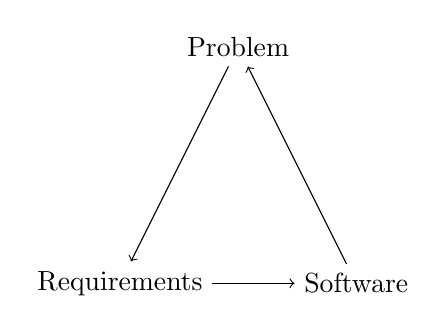
\begin{tikzpicture}
    \node[draw=white,align=left] (A) at (1.5,3) {Problem};
    \node[draw=white,align=left] (B) at (0,0) {Requirements};
    \node[draw=white,align=left] (C) at (3,0) {Software};

    \path [->] (A) edge node[left] {} (B);
    \path [->] (B) edge node[left] {} (C);    
    \path [->] (C) edge node[left] {} (A);    
\end{tikzpicture}
\end{center}

\textit{Product-based SE} is opposed to \textit{Project-based SE} and the above pictures changes as follows.

\begin{center}
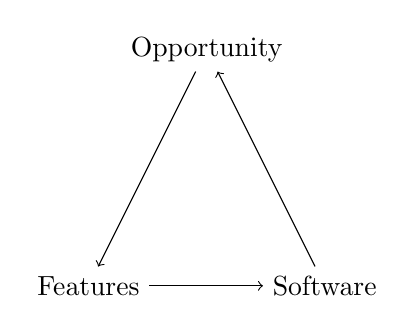
\begin{tikzpicture}
    \node[draw=white,align=left] (A) at (1.5,3) {Opportunity};
    \node[draw=white,align=left] (B) at (0,0) {Features};
    \node[draw=white,align=left] (C) at (3,0) {Software};

    \path [->] (A) edge node[left] {} (B);
    \path [->] (B) edge node[left] {} (C);    
    \path [->] (C) edge node[left] {} (A);    
\end{tikzpicture}
\end{center}

\section{Agile}
Agile is a collection of principles and methods applied in the software development field.
\nl

Opposed to project-based SE, in Agile the client is requested to express the requirements not in technical terms but in features.

Agile suggests an incremental development model

\subsection*{Principles}
\begin{enumerate}
    \label{subsec:agile_principles}
    \item Satisfy customer through early and continuous delivery of valuable software
    \item Welcome changing requirement, even late in development.
    Agile processes harness change for the customer's comptetitive advantage
    \item Deliver working software frequently, from a couple of weeks to a couple of months, with a preference to the shorter timescale
    \item Business people and devs must work together daily throughout the prokect
    \item Build porjects around motivated individuals and give them the environment and support they need
    \item The most efficient and effective method of conveying information to and within a dev team is face-to-face conversation
    \item Working software is the primary measure of progress
    \item Agile processes promote sustainable dev 
    \item Continuous attention to technical excellence and good design enhances agility
    \item Simplicity i.e. art of maximizing the amount of work not done is essential
    \item The best architectures, requirements, and designs emerge from self-organizing teams.
\end{enumerate}

Extreme Programming was proposed as part of the agile methodology

\section{Scrum}
Since requirements changes are rather frequent, long-term plans are unreliable,
hence SE aims to formulate short-term plans.

Scrum is found on \textbf{empiricism} and \textbf{lean thinking}; it asserts that knowledge comes from experience, and that decisions should be made on observations.

Other key terms are code \textbf{Transparency} among the team and with the customer, \textbf{Inspection} of produced code and software (artifacts), \textbf{Adaptation} to changes in features and requirements.

The \textbf{Scrum Team} is composed by:
\begin{enumerate}
    \item \textbf{Product Owner}: must ensure that the dev team is always focused on the goal
    \item \textbf{Scrum Master}: Scrum expert which drives the team to apply properly the Scrum framework.
    \item \textbf{Developers}: actual monkeys people which write code
\end{enumerate}

In scrum SW is developed in \textbf{sprints}, i.e. fixed-length periods with a specific goal to be achieved.

\begin{itemize}
    \item Product backlog: to-do list of items to be implemented
    \item Timeboxed sprints
    \item Self-organizing teams
\end{itemize}

...
\textbf{Prod Backlog Revised}\\
\textbf{PBI Estimation Metrics}

\subsection{Timeboxed Sprints}
Even if at the end of a srpint the goal hasn't been reached, "no worries", the work stops anyway;
there will be a new sprint which will include the work which has not been implemented in the previous one.

\subsection{Scrum Meetings}

\subsection{Agile activities}
Test automation
Continuous integration

\subsection{Sprint reviews}
At the end of each sprint there is a review meeting which involves the \textit{whole} team.
The \textit{product owner} has the ultimate authority to decide wether the sprint goal has been reached or not.
The sprint review should include a process review, in which the whole team shares ideas on how to improve their way of working.

\textbf{Team size}\nl

\section{5 - Ottobre}



\chapter{IEEE 802.11}

\begin{figure}[htbp]
   \centering
   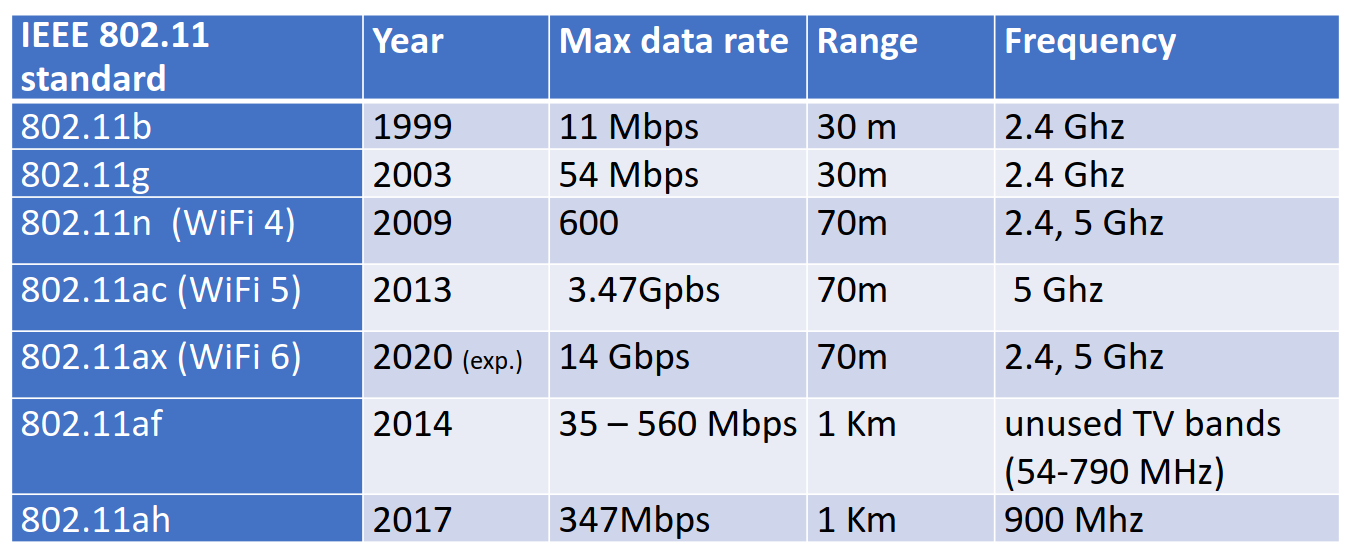
\includegraphics{images/ieee_bgn.png}
   \caption{IEEE 802.11 standards}
   \label{fig:ieee_bgn}
   All these standards \texttt{use \texttt{CSMA/CA} for multiple access}, and have base-station and ad-hoc network versions
\end{figure}

IEEE 802.11 standards refer to the \textit{Physical} Layer.
In case of an AP (Access Point), every station must channel its communication through the AP to talk to any other. Otherwise, in an \textit{Ad-Hoc} network, stations can communicate directly with each other.

TODO

\note{TODO non ci sono domande su questa cose nel pdf}
\chapter{Fabric}
``Fabric'' is the term used to refer to the \textit{interconnection} between nodes of a datacenter.\\
\ul{Cabling is of paramount importance.}
\note{Prof. Cisternino learnt it ``the hard way'' when he performed the cabling of the first UniPi datacenter by himself}
\begin{enumerate}
   \item Maintenance
   \item Cooling
   \begin{enumerate}
      \item Cables may heat up
      \item Cables may obstruct air flow
   \end{enumerate}
   \item Determines which machines interact with each other (\textit{fabric})
   \item Bandwidth
   \item Not neglectable cost
\end{enumerate}

We refer to North-South traffic indicating the traffic outgoing and incoming to the datacenter (internet), while we refer to East-West as the internal traffic between servers.
Most of the network (or fabric) traffic is processed horizontally (North-South traffic)\footnote{Seems odd that ``horizontal'' refers to North-South traffic, but that's how it is.}.


\section{Bandwidth and Storage implications}
\label{sec:bandwidth_storage}
A standard datacenter has servers connected with 25Gbit links in both directions, summing up to 50Gbit total bandwidth.
Current SSDs using NVMe provide much more, about $3.5 GB/s$, making \ul{4 drives are enough to saturate a 100Gbit/s link.}\\
We moved from a situation where the \textbf{bottleneck} were slow Hard Drives, to the current one where the bottleneck is the ---network--- \textbf{bandwidth}.\\
Recently the PCI 3.0, which lasted very long ---providing roughly$\sim\texttt{120Gbit/s}$ using 16 pin---, suddenly become unsufficient to handle the needed traffic.

Considering this, \ul{datacenters must be designed to allow \textit{Terabytes} of data to be moved in east-west traffic.}

\begin{center}
   \ul{\textit{The \textbf{fabric} is the glue that makes the datacenter possible.}}
\end{center}

Besides, a single server is \textit{unable} to handle 10TBs of data and handling requests from 3000 users simultaneously. It is necessary to \textbf{distribute} the requests.

HDDs are still currently used for \textbf{cold storage};
CPUs will access data exclusively from SSDs, and sometimes the server is shipped with on board \textbf{full-flash storage}.\\
The difference in price between SSDs and HDDs becomes negligible since you pay for top CPU, top GPU, top RAM;
furthermore, you can't waste ---the high amount of--- energy ---consumed by such components--- by waiting for a slow drive.

SSDs have a known write limit, but today, the usually last enough time: if you write the whole disk every day it will last for 5 years. Most-likely after five years you'd have to renew some components anyway, besides the failure is a predictable event.

\section{Cables and standards}
\subsection{Optical}
Electric current propagates at a speed $s = {\sim}0.6c$.
Hence \textbf{optical fiber} is ---at least in theory?--- faster.

\textbf{Lasers} are a coherent beam of equal fotons. It is possible to transfer energy through such fotons. Something resembling a laser is used for optical fibers.

Blu-Ray came out when scientists managed to create light using frequencies in the Blu area, which are the higher ones.
Currently, the best and most expensive optical fibers exploit blu-lasers as source of light.

Note that with optical you always need 2 fibers, one sending and the other receiving. The two possible connectors are \texttt{SC} and \texttt{LC}.
Sometimes the two ends of the cable are detachable so that the cables may be switched; this is useful because sometimes you may want to attach the TX cable on the RX plug and viceversa. 

\begin{figure}[htbp]
   \centering
   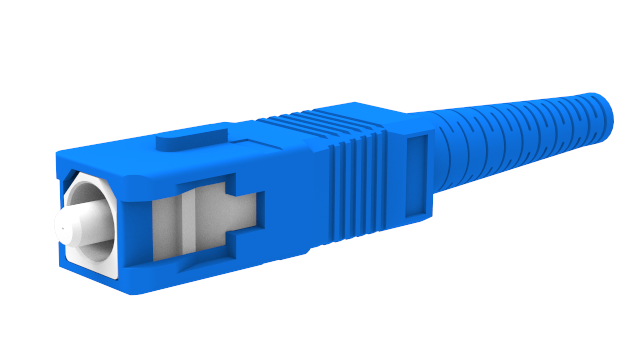
\includegraphics[width=0.25\columnwidth]{images/SC.png}
   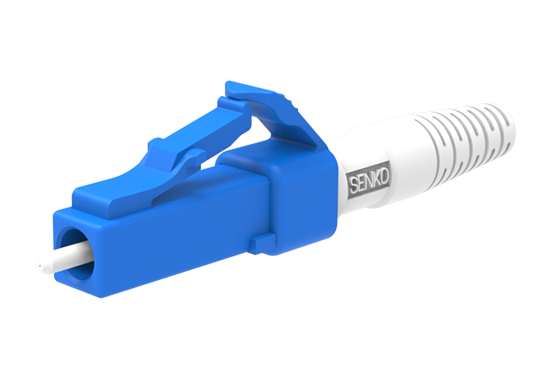
\includegraphics[width=0.25\columnwidth]{images/LC.png}
   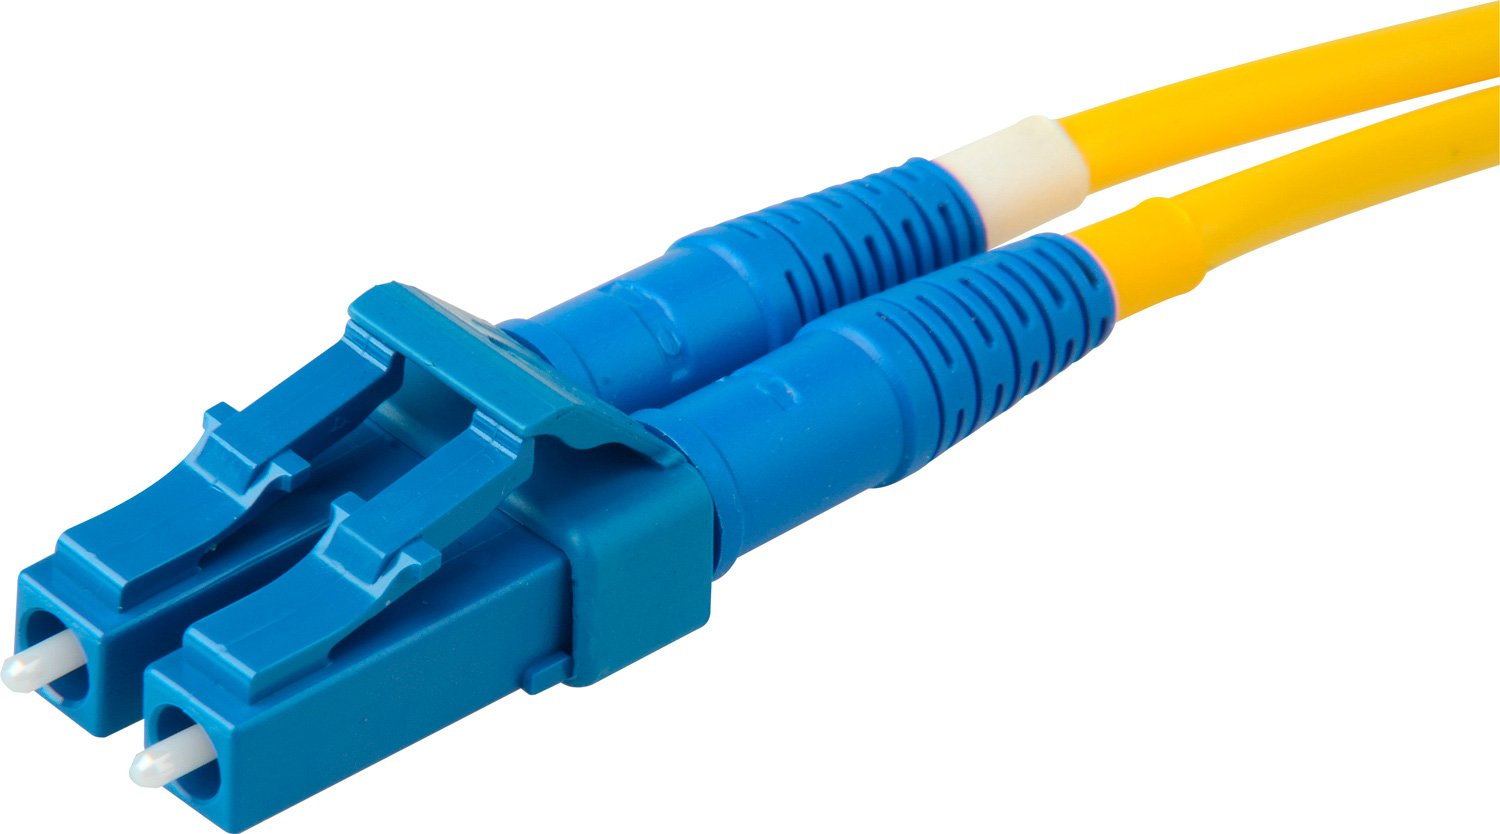
\includegraphics[width=0.25\columnwidth]{images/LC_coupled.JPG}
   \caption{\texttt{SC} and \texttt{LC} connectors}
   \label{fig:sc_lc_connectors}
\end{figure}

\subsection{Copper wires}
In case of electricity there are many aspects to be considered. Interferences, cable diameter/size, length, and also the fact that if a \texttt{1} has been transmitted for some time, it takes longer to transmit a \texttt{0}, due to the \textit{commutation} that must happen.
\nl

\begin{paracol}{2}
   \colfill
   \textbf{RJ45} is a standard physical interfaced for copper wires, which allows up to 1Gbit regularly.
   The \texttt{Cat 7} cables still use the RJ45 as connector and provide instead 10Gbit/s, but are very uncomfortable, they are so thick that they are difficult to bend.
   
   It is estimated that there have been installed $70 \times 10^9m$ of Ethernet cables, making them the most used.
   \colfill
   \switchcolumn

   \begin{figure}[htbp]
      \centering
      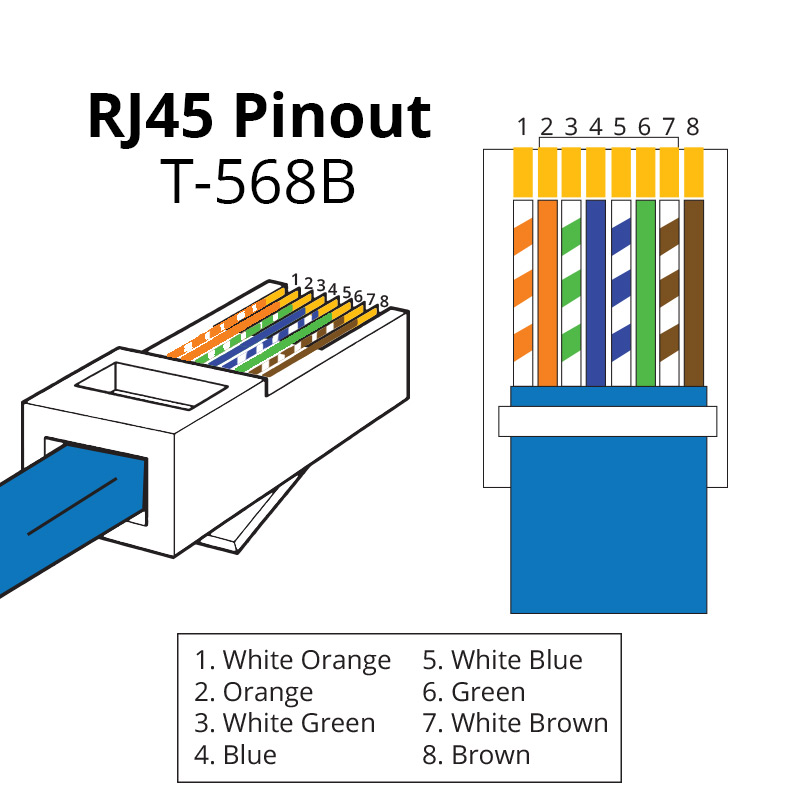
\includegraphics{images/RJ45_T568B.jpg}
      \caption{RJ45 - T568B}
      \label{fig:RJ45_T568B}
   \end{figure}
\end{paracol}

\subsection{SFP - Small Form-factor Pluggable}
There can be a cable with a LC in one side and a SC on the other side.
Instead of making switches with the optical plugs, switches were created with electrical plugs that would be able to host a \textbf{standard transceiver}.
The latter is a pluggable module that will receive current power and electrical signals for the transmission, which is responsible for transitioning between electrical signals and Optical signal (and viceversa).

\begin{paracol}{2}
   
   The aim of SFP is to decouple the optical transceivers from the server modules.
   \note{Is this correct?}
   They allow to go \textit{optic-copper}, \textit{copper-optic}, \textit{optic-optic} and \textit{copper-copper}.\\
   SFP and GBIC (oldest one, now dead) pluggable modules acting as active transceivers for optical wiring using RJ45 connector.\\
   \ul{A single cable having SFP ends costs about 100€}.
   The cost ain't neglectable \smiley.
   \note{\begin{itemize}
      \item[\texttt{SFP}] $\longrightarrow 1Gbit $
      \item[\texttt{SFP+}] $\longrightarrow 10Gbit $
      \item[\texttt{SFP28}] $\longrightarrow 25Gbit$
      \note{This is the current standard}
      \item[\texttt{QSFP28}] $\longrightarrow 4\times25Gbit$
   \end{itemize}}


   \switchcolumn

   \begin{figure}[htbp]
      \centering
      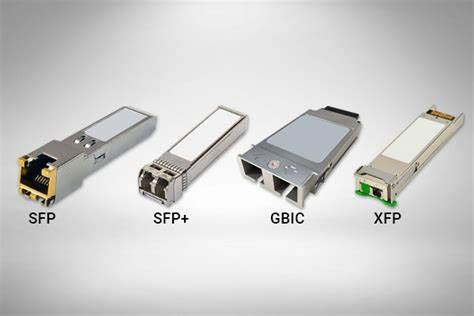
\includegraphics{images/sfp.jpeg}
      \caption{SFP transceivers form factors}
      \label{fig:sfp}
   \end{figure}
\end{paracol}

\note{Fun fact: ci sono 9 cavi USB-C e solo due portano informazioni video.}

\subsubsection{Issues about cabling and fabric}
The key point is that it would be desirable for cabling to be reconfigurable, that's why transceivers are so important.

\note{There are things called \textit{``Muffole''}, which are used for joining optical fiber cables, allowing for longer distances to be covered.
They are designed to be underground.}

Data traffic is always at least SFP+.
Current standard is SFP28. Various SFP are typically compatible, the shape of the plug should stay the same.
On switches there also some ports which are \texttt{QSFP+} or \texttt{QSFP28}, which allow up to \texttt{40} and \texttt{100Gbit/s} respecitively, and are used for north-south traffic.
\note{The \texttt{Q} letter stands for \textit{Quality}}

Switches for datacenters should be \textbf{non-blocking}, meaning that no port has to wait for other ones ---or any other thing--- before transmitting, they can also transmit simultaneously.


\ul{In every datacenter it is \textit{MANDATORY} to document the cabling.}

\subsection{InfiniBand}
Even though Ethernet is famous, it is not the only standard. InfiniBand is another one, which is used in supercomputers and known for its very high throughput and very low latency ($\sim 2\mu s$).
It may send messages up to 2GB each, with 16 priority levels.
It is a \textit{lossless protocol}, meaning that if a packet is received, its integrity is guaranteed.

\textit{IB} avoids TCP/IP stack, which is very heavy, and instead uses MPI (\textit{Message Passing Interface}), which is a way to distributed parallel programs, also exploited by OmniPath.

InfiniBand cables and connectors look similar to Ethernet ones, but they are not compatible.

Aside from HPC environments, it is uncommon to build an entire network with InfiniBand, typically there is an IB switch to whom the servers equipped with IB NICs are connected, which intereacts with the rest of the network with Ethernet, because ``it's cheaper and it works''.
\note{Today, we are about 400 Gbit/s on both IB and Ethernet.}

\subsection{RDMA - Remote Direct Memory Access}

RDMA is a technology API based (not a protocol!) that allows to access memory of a remote machine without involving the CPU or the OS of the remote machine.

RDMA supports zero-copy networking by enabling the network adapter to transfer data directly to or from application memory, eliminating the need to copy data between application memory and the data buffers in the operating system.\\
The main use case is distributed storage.

RoCE (\textit{RDMA over Converged Ethernet}) is a network protocol that allows remote direct memory access (RDMA) over an Ethernet network.

\subsection{Omni-Path}
Omni-Path is a high-performance computing network architecture, developed by Intel. It is a successor to Intel's InfiniBand, and competes with InfiniBand's EDR and HDR technologies.

Intel plans to develop technology that will serve as the on-ramp to \textit{exascale computing}\footnote{A computing system capable of the least one exaFLOPS}, which is the next frontier in high-performance computing.


\chapter{BitTorrent}

The goal of \textit{Content Distribution Networks} is to distribute web contents to hundreds of thousands or millions
of simultaneous users, \ul{exploiting data and/or service \textbf{replication} on different \textbf{mirror servers}}.

In \textbf{P2P CDN} the initial file request are served by a centralized server, and further requests served by peers which have already received and replicated the files (\textbf{\textit{seeders}}), without involving the initial server.

\begin{center}
\fbox{
   \begin{minipage}{0.8\columnwidth}
      \nl
      \begin{center}
         \ul{\textbf{BitTorrent} in a nutshell}
      \end{center}
      \nl

      \begin{itemize}
         \item Basically a \textit{Content Distribution Network} (\texttt{CDN})
         \item A distributed set of hosts cooperating to distribute large data set to end users.
         \item Efficient content distribution systems using \textit{file swarming}
         \item Does \textit{not} perform all the functions of a typical P2P system, like searching
         \item Rather than providing a search protocol itself, was designed to integrate seamlessly with the Web and made file descriptors available via Web, which could be searched with standard Web search
         \item \textit{File swarming}: a peer makes whatever portion of the file that is downloaded immediately available for sharing
      \end{itemize}
   \end{minipage}  
   }
\end{center}

\section{Deeper into BitTorrent}
\begin{figure}[htbp]
   \centering
   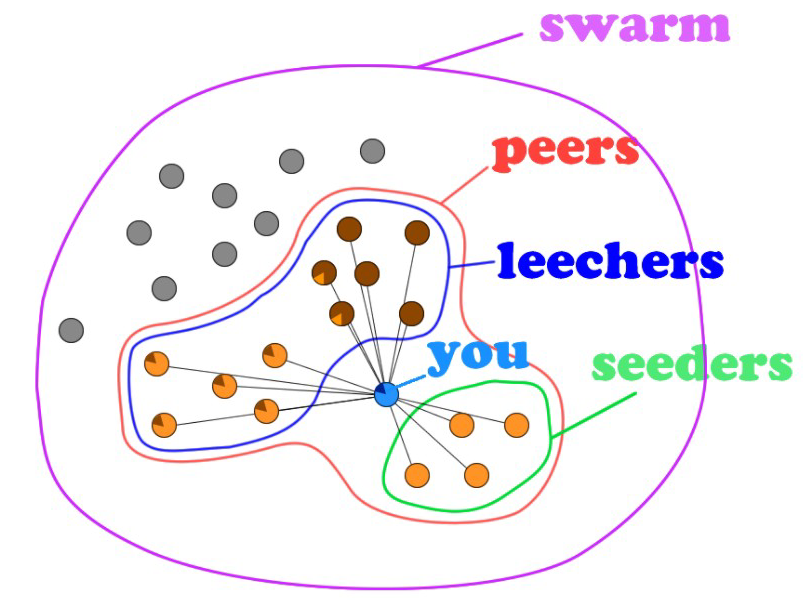
\includegraphics{images/bit_swarmschema.png}
   \caption{Swarm schema}
   \label{fig:bit_swarmschema}
\end{figure}
\subsection{Glossary}
\begin{itemize}
   \item \textbf{tracker}: active entity which coordinates
   the peers sharing the file, taking trace of who is currently providing the content
   \note{\begin{itemize}
      \item Joe connects to the tracker announcing the content
      \item the tracker now knows Joe is providing the file
   \end{itemize}}
   \item \texttt{.torrent} a descriptor of the file to be published on a server, which includes a reference to a tracker
   \item \textbf{swarm} set of peers collaborating to the distribution of the same file coordinated by the same tracker
   \item \textbf{seeder} peer which owns all the parts of the file
   \item \textbf{leecher} peer which has some part or no part of the file and downloads the file from the seeders and/or from other lechers.
\end{itemize}

\subsection{Protocol Overview}
\begin{figure}[htbp]
   \centering
   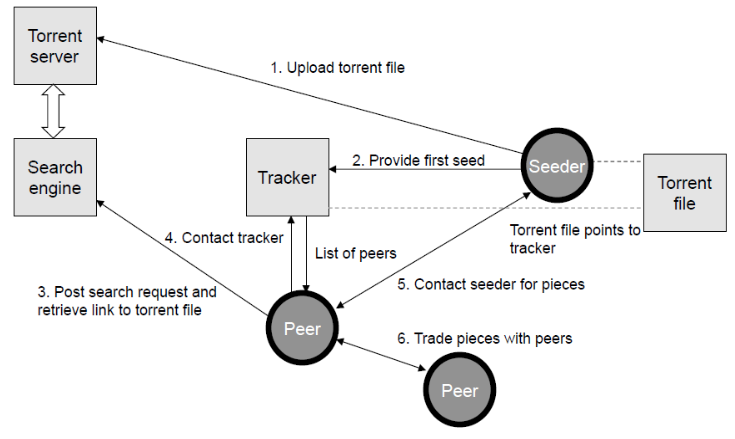
\includegraphics{images/bit_overview.png}
   \caption{BitTorrent protocol overview}
   \label{fig:bit_overview}
   BitTorrent protocol is built on top of HTTP
\end{figure}
\labelitemize{\textit{Seeder}}{
   \begin{enumerate}
      \item Upload the .torrent on a Torrent Server
      \item Opens a connection to the Tracker and informs it of its own existence: for the moment, it is the only peer which owns the file
   \end{enumerate}
}
\labelitemize{\textit{Peers}}{
   \begin{enumerate}
      \setcounter{enumi}{2}
      \item Retrieves the file descriptor (.torrent) and opens it through the BitTorrent
      client
      \item Opens a connection to the tracker and informs it of its own existence and
      receives from the tracker a list of peers of the swarm
      \item Opens a set of connections with other peers of the swarm.
   \end{enumerate}
}

Objects are serialized in \textbf{Bencode}, which is ---not popular as \texttt{JSON}--- used only in torrent; provides 4 data types: String, Integer, Lists and Dictionaries.\\
Content is split into chunks called pieces (256KB - 2MB):
when a peer receives a piece, it becomes the seeder of that piece.
\note{
   \ns
      There is a SHA-1 hash per piece stored in the .torrent file, used to check the piece once it is fully downloaded, 
      allowing to require retransmission in case the check fails.\\
      Pieces size got adapted to have a reasonably small .torrent file
}
Pieces are then split in \textbf{subpieces} (\textit{\textbf{blocks}}) of 16KB, with each one downloadable from a different peer, optimizing the bandwith and allowing \textit{pipelining}, decreasing the overall download time.

Trackers keep a database of swarms identified by torrent hash, and knows also the state of each peer in each swarm.
In the last versions, \textbf{trackerless} BitTorrent uses \textit{Kademlia DHT} to avoid the centralization point of the tracker.

\section{Pieces selection}
The order in which pieces are selected by different peers is critical for good performance, to avoid making peers end up stuck with the same pieces.
\labelitemize{\textit{Policies}}{
   \begin{itemize}
      \item \textbf{Strict Priority}\\
      Complete the ``assembling'' of a piece before asking for another piece
      \item \textbf{Rarest First}\\
      Download the rarest pieces first
      \item \textbf{Random First Piece}\\
      Choose a random piece ---only--- in the bootstrap phase
      \item \textbf{Endgame}\\
      When the file download is almost terminated, the remaining pieces are required in \textit{parallel} to all peers who own them.
      This policy is executed for a small period of time
   \end{itemize}
}

\subsection{Free Riders}
Free riders in BitTorrent are peers that do not put their bandwidth at disposal of the community.\\
Several non official BitTorrent clients enable the user to limit the upload bandwidth as they like.

However, an approach to solve this problem is based on \textbf{reciprocity}, allowing a client to obtain a good service if and only if it gives a good service to the community, by exploiting a dynamic strategy based on connection monitoring called ``Tit for Tat'', implemented using \textbf{choking}:\\
choking means \textit{temporarily} refusing to upload to another peer, but still downloading from them;  
the principle is to upload to peers who have uploaded to us.

\labelitemize{\textit{Choking}}{
\begin{center}
   \textit{The local peer can receive data from a remote peer if}
   \begin{itemize}
      \item The local peer is \textit{interested} in the remote peer
      \item The remote peer \textit{unchoked} the local peer
   \end{itemize}
\end{center}
   }

Choking only peers that upload the most to the local peers would lead to ignoring peers that recently join the network
and to the lack of discovery of connections actually better than the used ones.\\
To avoid this, BitTorrent uses \textbf{optimistic unchoking}, i.e. \ul{one random peer is being unchoked}.\\
Then, every 30s an interested and choked peer is selected at random \textbf{planned optimistic unchoke} (\texttt{POU}), and if this new connection turns out to be better than one of the existing
unchoked connections, it will replace it.

In case a peer is chocked by everyone, it follows an \textbf{anti-snubbing} policy, by increasing the number of simultaneous optimistic
unchocke to more than one.

For \textit{seeders} this schema does clearly not apply, since they do not have to download anything; hence they use a different choking algorithm:
\ul{unchoke peers with the highest upload rate}, ensuring that pieces get uploaded and replicated faster.

\section{DHT and BitTorrent}
Kademlia is the protocol used by the largest public DHTs.
Bittorrent Inc. introduces its own DHT, called \textit{Mainline DHT}.
With respect to Kademlia there are some improvements concerning 
\begin{itemize}
   \item Routing table management
   \item Look-up
\end{itemize}

The main purpose of Mainline DHT is to provide a “trackerless” peer discovery mechanism to locate peers belonging to a swarm.
\chapter{Storage}

\framedt{Data Loss}{
   \textit{``Storage is crucial because, if a switch fails, or a server fails, the service will be interrupted, but the data will still be there. \ul{If the storage fails, the \textbf{data will be lost}}.''}
   -Prof. Cisternino\\

   \textbf{Data} is the most important of a system. Since data loss is \textbf{permanent}, the storage is completely different from computing or networking.
}

\begin{paracol}{2}
   \colfill
   Historically the storage was the slowest part of the system, \textit{ms} against \textit{ns} of the CPU.
   Today, with SSDs, the gap is considerably reduced to \textit{$\mu s$}, they are $\sim 100x$ times faster.
   
   \ul{NVMe stands for \textit{Non-Volatile Memory Express}, and is a protocol (\textit{not a HW component!})} that allows to access the storage directly from the PCIe bus, without having to go through the SATA controller. This allows to have a much higher throughput, and a much lower latency.

   \note{Optane was a technology developed by intel which is now end of life}

   \colfill
   \switchcolumn

   \begin{figure}[htbp]
      \centering
      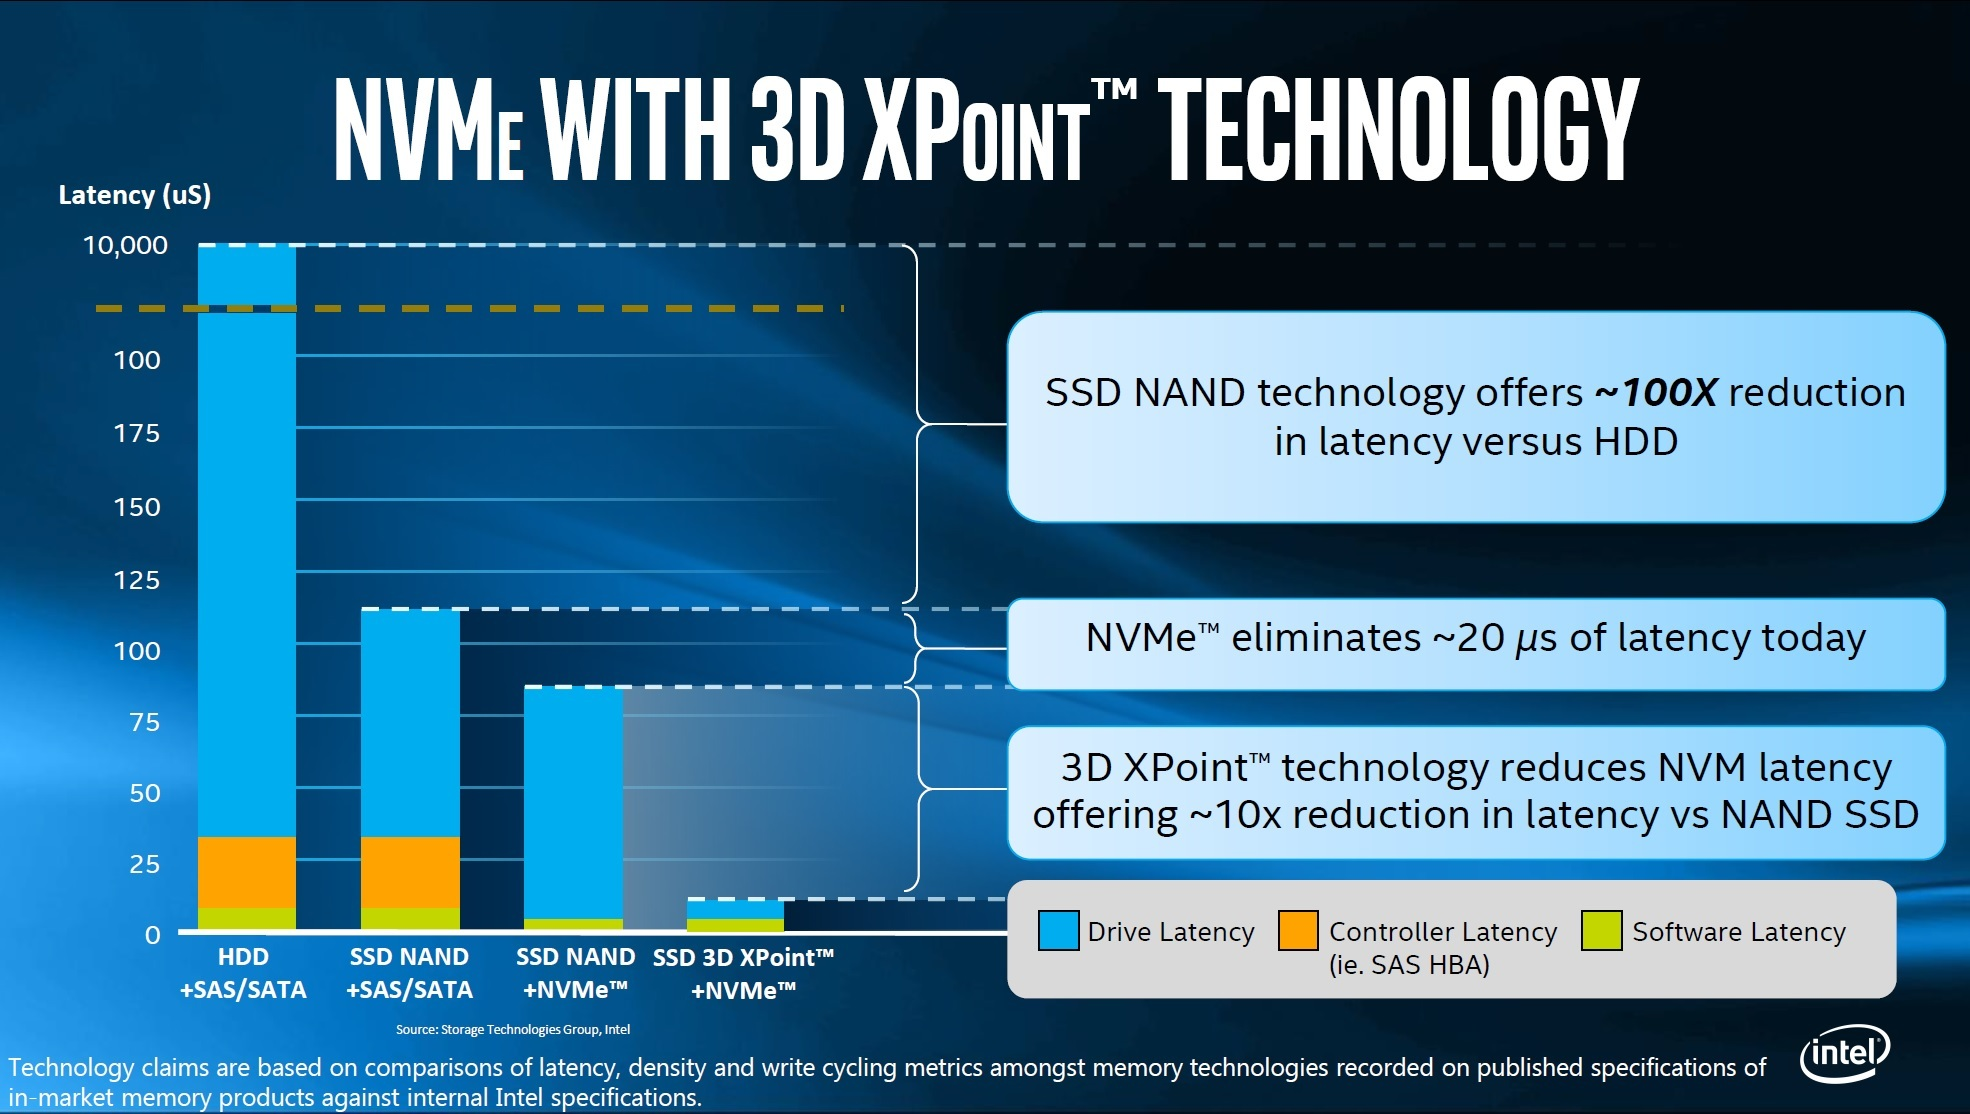
\includegraphics{images/storage_intel.jpg}
      \caption{Storage types comparison}
      \label{fig:storage_intel}
      NVMe basically removes the orange part of the figure, which is the latency introduced by the controller, since it is a \textit{controller-less protocol} and allows to access the storage directly from the PCIe bus.
   \end{figure}
\end{paracol}


\framedt{
   \textit{Why would a 15TB disk be better than a 27TB disk?}\\
   }{
      \note{Assume the same performance, and the same price.}
      It would be preferrable because \ul{it would take less time to extract all the data from the disk}\footnotemark[1], since it is smaller.
      
      However, large capacity drives are used for \textit{cold storage}, where the data is not accessed frequently, speed is not a priority, and even if the data is accessed, only a portion of the disk is needed at a time; in case of failure and thus needing to retrieve an entire backup, the time taken to retrieve the data is not a priority, since this ---hopefully--- happens only ``once''.
      }
      
\footnotetext[1]{i.e. taking advantage of the space provided}
\section{SSDs - QLC and TLC}
SSDs were invented by Toshiba back in 1980, but they were not popular for almost 30 years, until they eventually became cost-effective. Sometimes extra size in SSDs is used for redundancy, to increase the lifespan of the disk e.g. on a 30TB disk, only 10TB are used, the rest is used for redundancy, extending x3 the lifespan of the disk.

\note{DWPD stands for \textit{Drive Writes Per Day}, and is a measure of how many times the disk can be written to in a day. It can be calculated as $\frac{TBW}{365\times\textit{Years of Warranty}\times\textit{capacity}}$}.

TLC stands for \textit{Triple Level Cell}, and QLC stands for \textit{Quad Level Cell}. The difference between the two is the number of bits stored in each cell. The more bits stored in each cell, the cheaper the disk is, but the slower it is. The more bits stored in each cell, the more difficult it is to read and write the data, and the more difficult it is to keep the data stored in the cell.

Generally QLC disks are used for cold storage, while TLC disks are used for hot storage.
TLC in general is more reliable than QLC, has a longer lifespan and better performance, however they cost more.

\section{Storage Concepts}
\subsection{Tiering - Memory Hierarchy}

\begin{figure}[htbp]
   \centering
   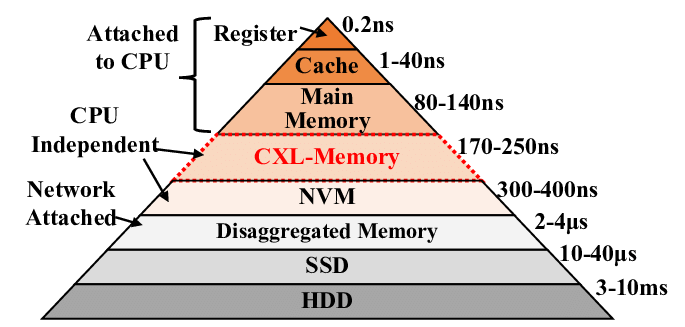
\includegraphics{images/tiering_memory.png}
   \caption{Memory tiering hierarchy}
   Ram could actually be split in \texttt{RAM} and \texttt{nvRAM} (Non-volatile \texttt{RAM}, uses \texttt{nvDIMM}), which is used to store the data in case of a power failure.
   Sometimes, \textit{tape} is included in the hierarchy, because it is used for long-term storage, and it is very cheap.
   \label{fig:tiering_memory}
\end{figure}

Tiering consists in categorizing the data in different categories, and storing the data in different types of storage, depending on the category. The data that is accessed more frequently is stored in the fastest storage, while the data that is accessed less frequently is stored in the slowest storage. This allows to increase the performance, and to reduce the cost. 

\subsection{IO operations, are they all the same?}
\textbf{IOPS} (Input/output operations per second) is an input/output
performance metric used to characterize computer storage devices; it is associated with an access pattern: \textit{random} or \textit{sequential}.

\subsubsection{Random vs Sequential access}

Before explaining the distinction, is important to remember the concept of \textit{queues}: for each thread, the OS can implement a series of queues to solve asynchronously the I/O requests. Using multiple queue can make performances better, since having
the OS to manage parallel requests will increase throughput.
If the queries are latency sensible, not using a queue is better, since
it allows a single query to have ``max'' priority.

\textit{Random access files} are advantageous in scenarios where frequent direct access or modification of specific records is required, while \textit{sequential access files} are advantageous in scenarios where frequent reads of the full files are required. The disk behaves differntly in case of access of those files.

To have a full picture of random vs sequential access, check this site: \url{https://www.prepbytes.com/blog/general/difference-between-sequential-and-random-access-file/} 

\newpage
\subsubsection{Cisternino's demo}
Prof. Cisternino showed a demo in class, where he used a tool to measure the IOPS of a disk.
\begin{figure}[htbp]
   \centering
   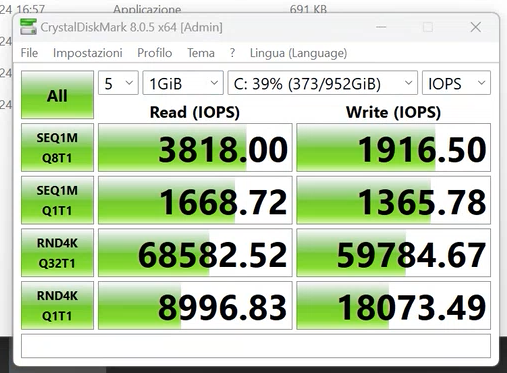
\includegraphics{images/iops.png}
   \caption{IOPS demo; respetively}
   \label{fig:iops}
\end{figure}

\ul{Recall that IOPS by itself is meaningless!} It is a number that must qualified and put in relationship with something else.

\subsection{Latency and Storage Aggregation}
A mechanical hard drive introduces 2.71\% of latency when reading, for instance, 40MB of data.  Optane can perform 416 accesses in the same time needed by a mechanical hard drive to perform 1 access. It looks like the latency in this latter case is neglegtible. Someone may be tempted to reduce the size of read/write operations and perform multiple smaller ones, since ``it's free''. 

Latency in general is due to:
\begin{itemize}
   \item \textbf{Software}\\
   $\mu s$ order which cannot be removed
   \item \textbf{Controller}\\
   Taken down to $20\mu s$ with NVMe (even $2.8\mu s$ according to Copilot)
   \item \textbf{HDD latency}\\
   This was drastically reduced with SSDs and got even less with 3D NAND.
\end{itemize}
Latency may be solved by \textbf{storage aggregation}, which consists in aggregating multiple storage devices into a single logical unit, in order to increase the performance and reliability.
Even if the data is split in multiple disks, the whole system is ``pictured'' as a single huge drive\footnote{\textit{``Cloud resource pooling''} rings a bell?}, making a huge difference in terms of latency, since multiple \texttt{read/write} requests may be sent in parallel to multiple disks.

\newpage
\subsection{Storage Fabric - Fibre Channel}
\textbf{Fibre Channel} is the fabric dedicated to storage; the link coming from the storage ends up in the \textit{HBA} (Host Bus Adapter) in the server.
\begin{paracol}{2}

   \colfill
   The idea is to have an interface which announces itself as drive and that manages the remote storage through Fibre Channel.
   Fibre Channel typically runs on optical fiber cables, but may also run on Ethernet cables (FCoE).

   In Fig. \ref{fig:fibrechannel} is depicted the ideal architecture for Fibre Channel, where the storage is connected to the network through a switch, and the servers have a dedicated HBA to connect to the storage.
   \colfill
   
   \switchcolumn
   \begin{figure}[htbp]
      \centering
      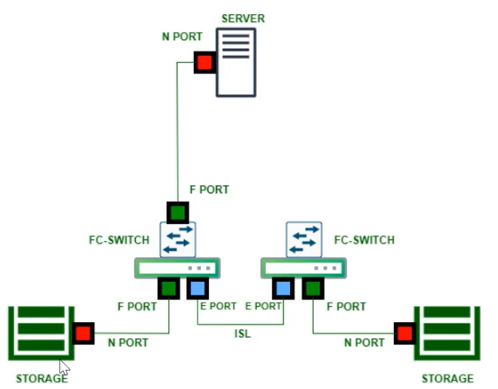
\includegraphics{images/fibrechannel.png}
      \caption{Fibre Channel desired architecture}
      \label{fig:fibrechannel}
   \end{figure}
   
\end{paracol}

\begin{figure}[htbp]
   \centering
   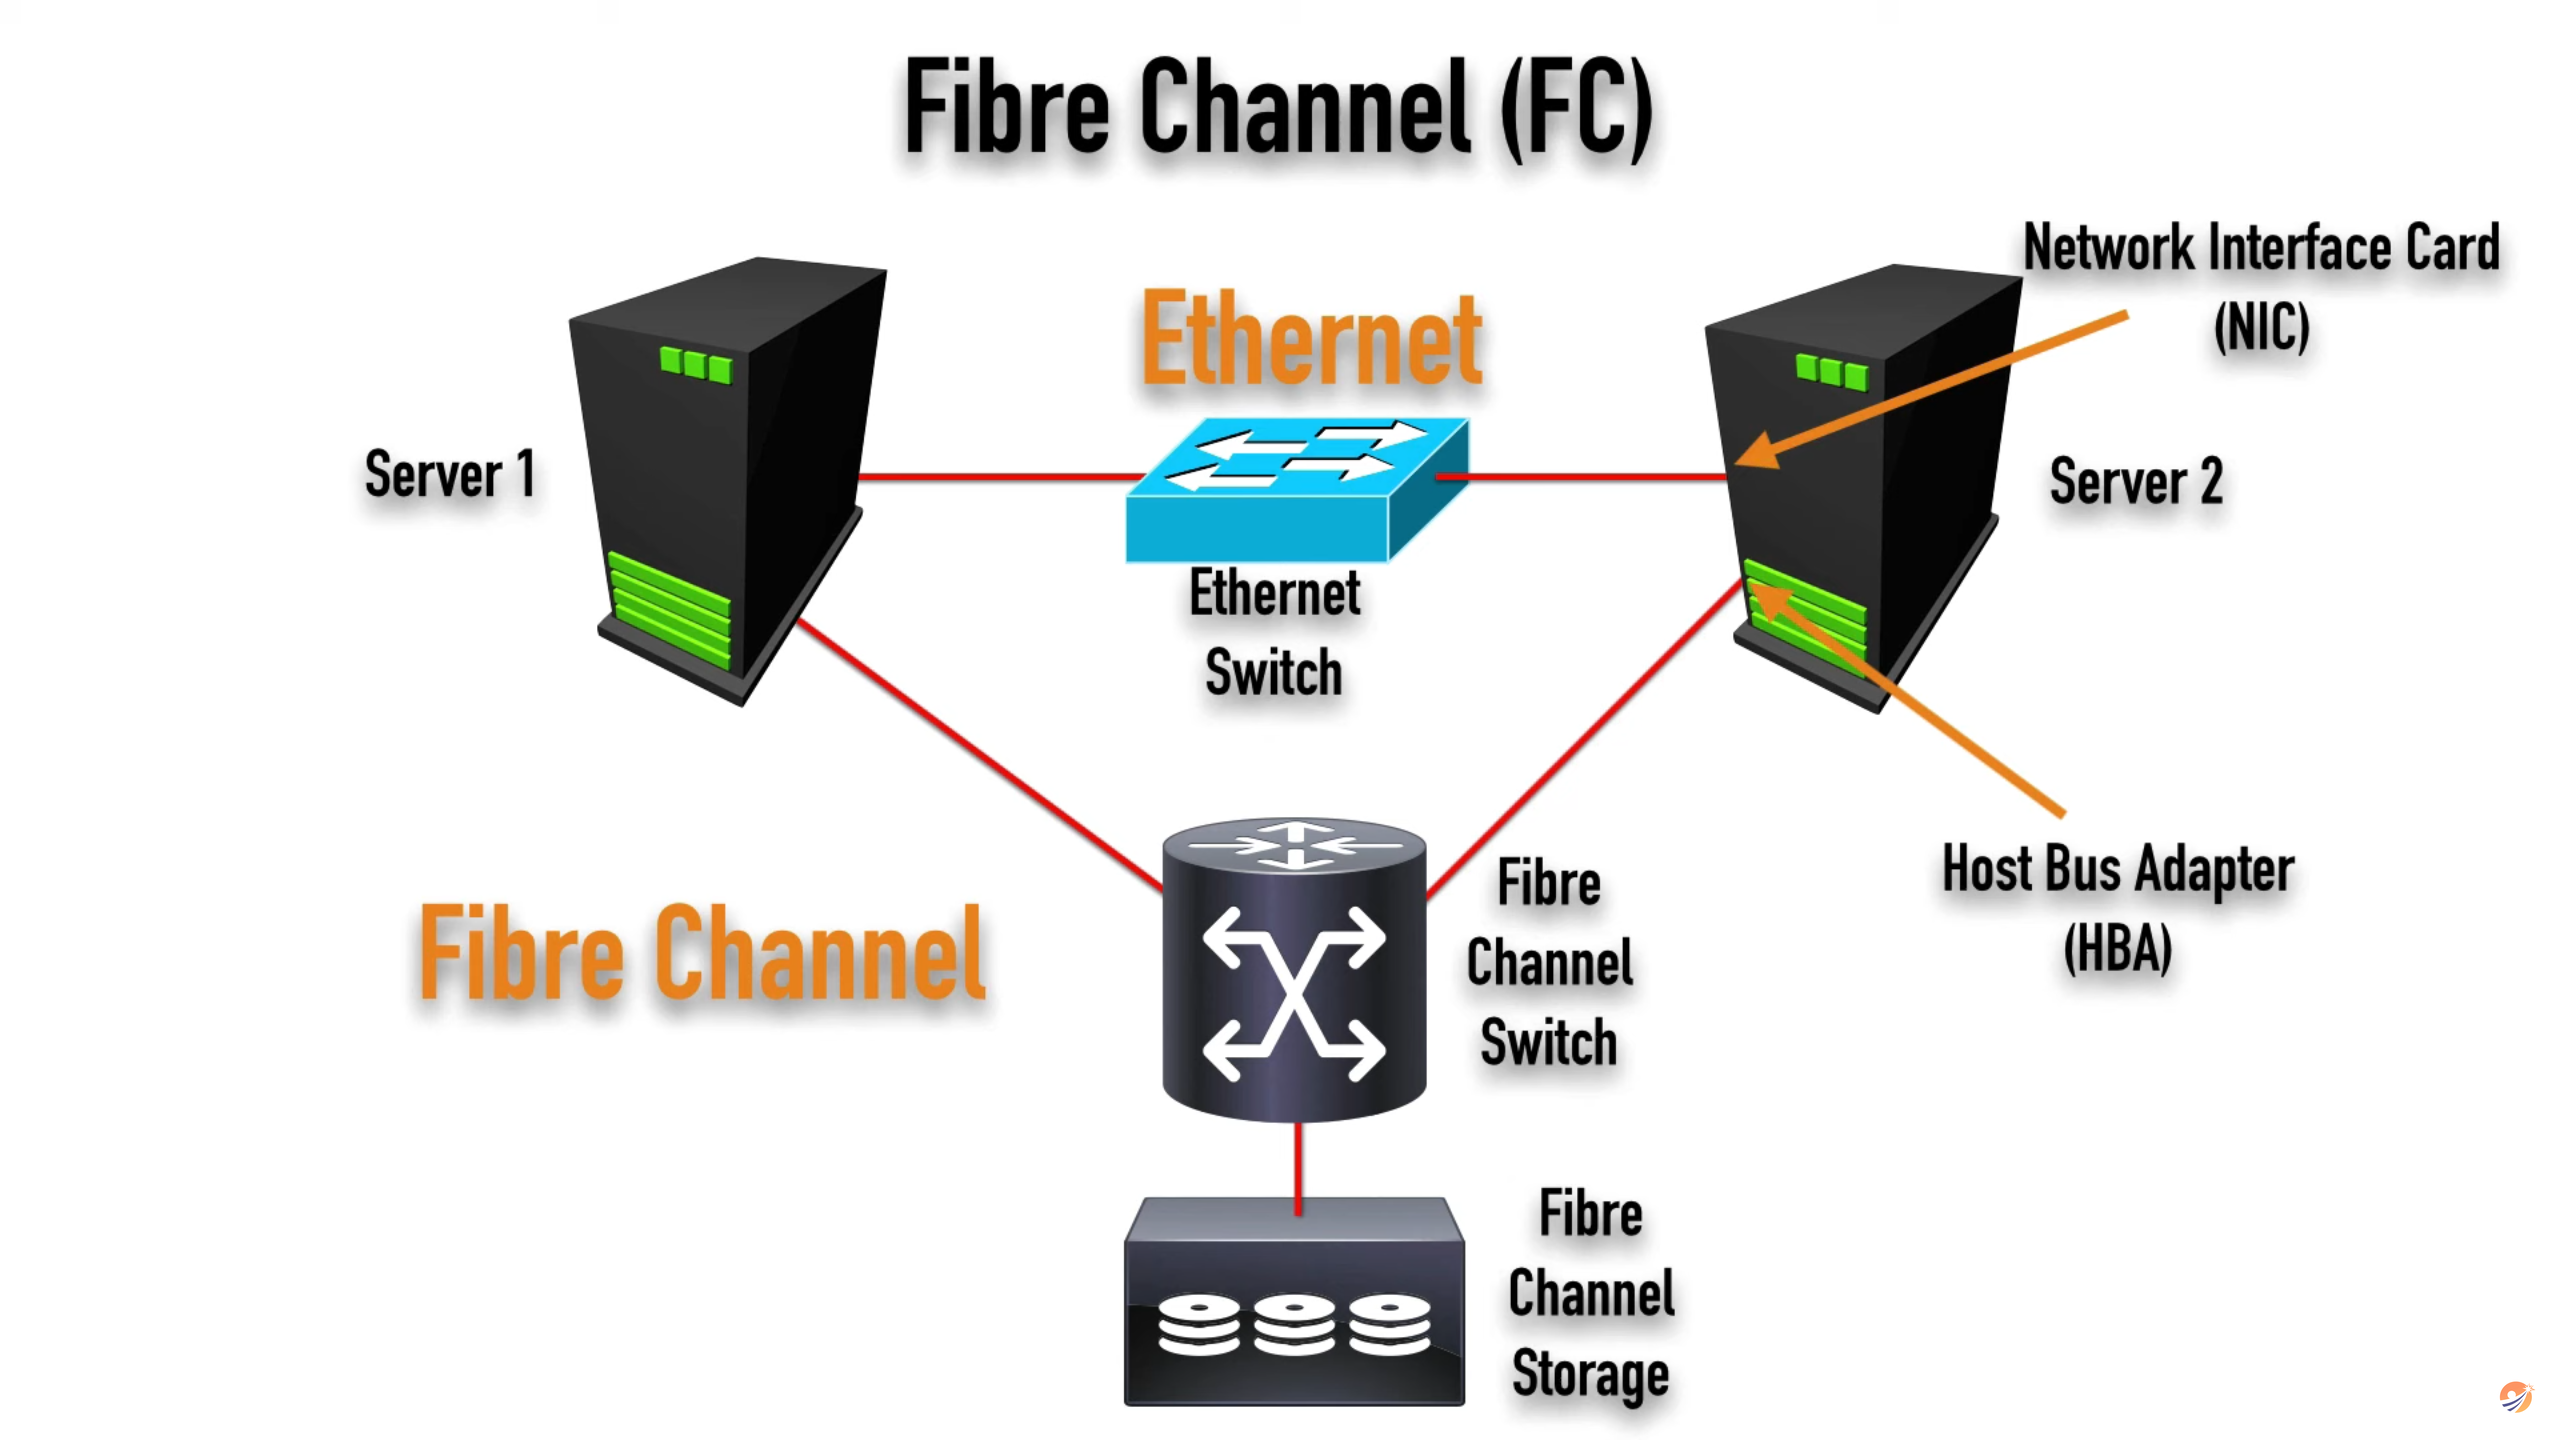
\includegraphics[width=0.32\columnwidth]{images/storage_fabric1.png}
   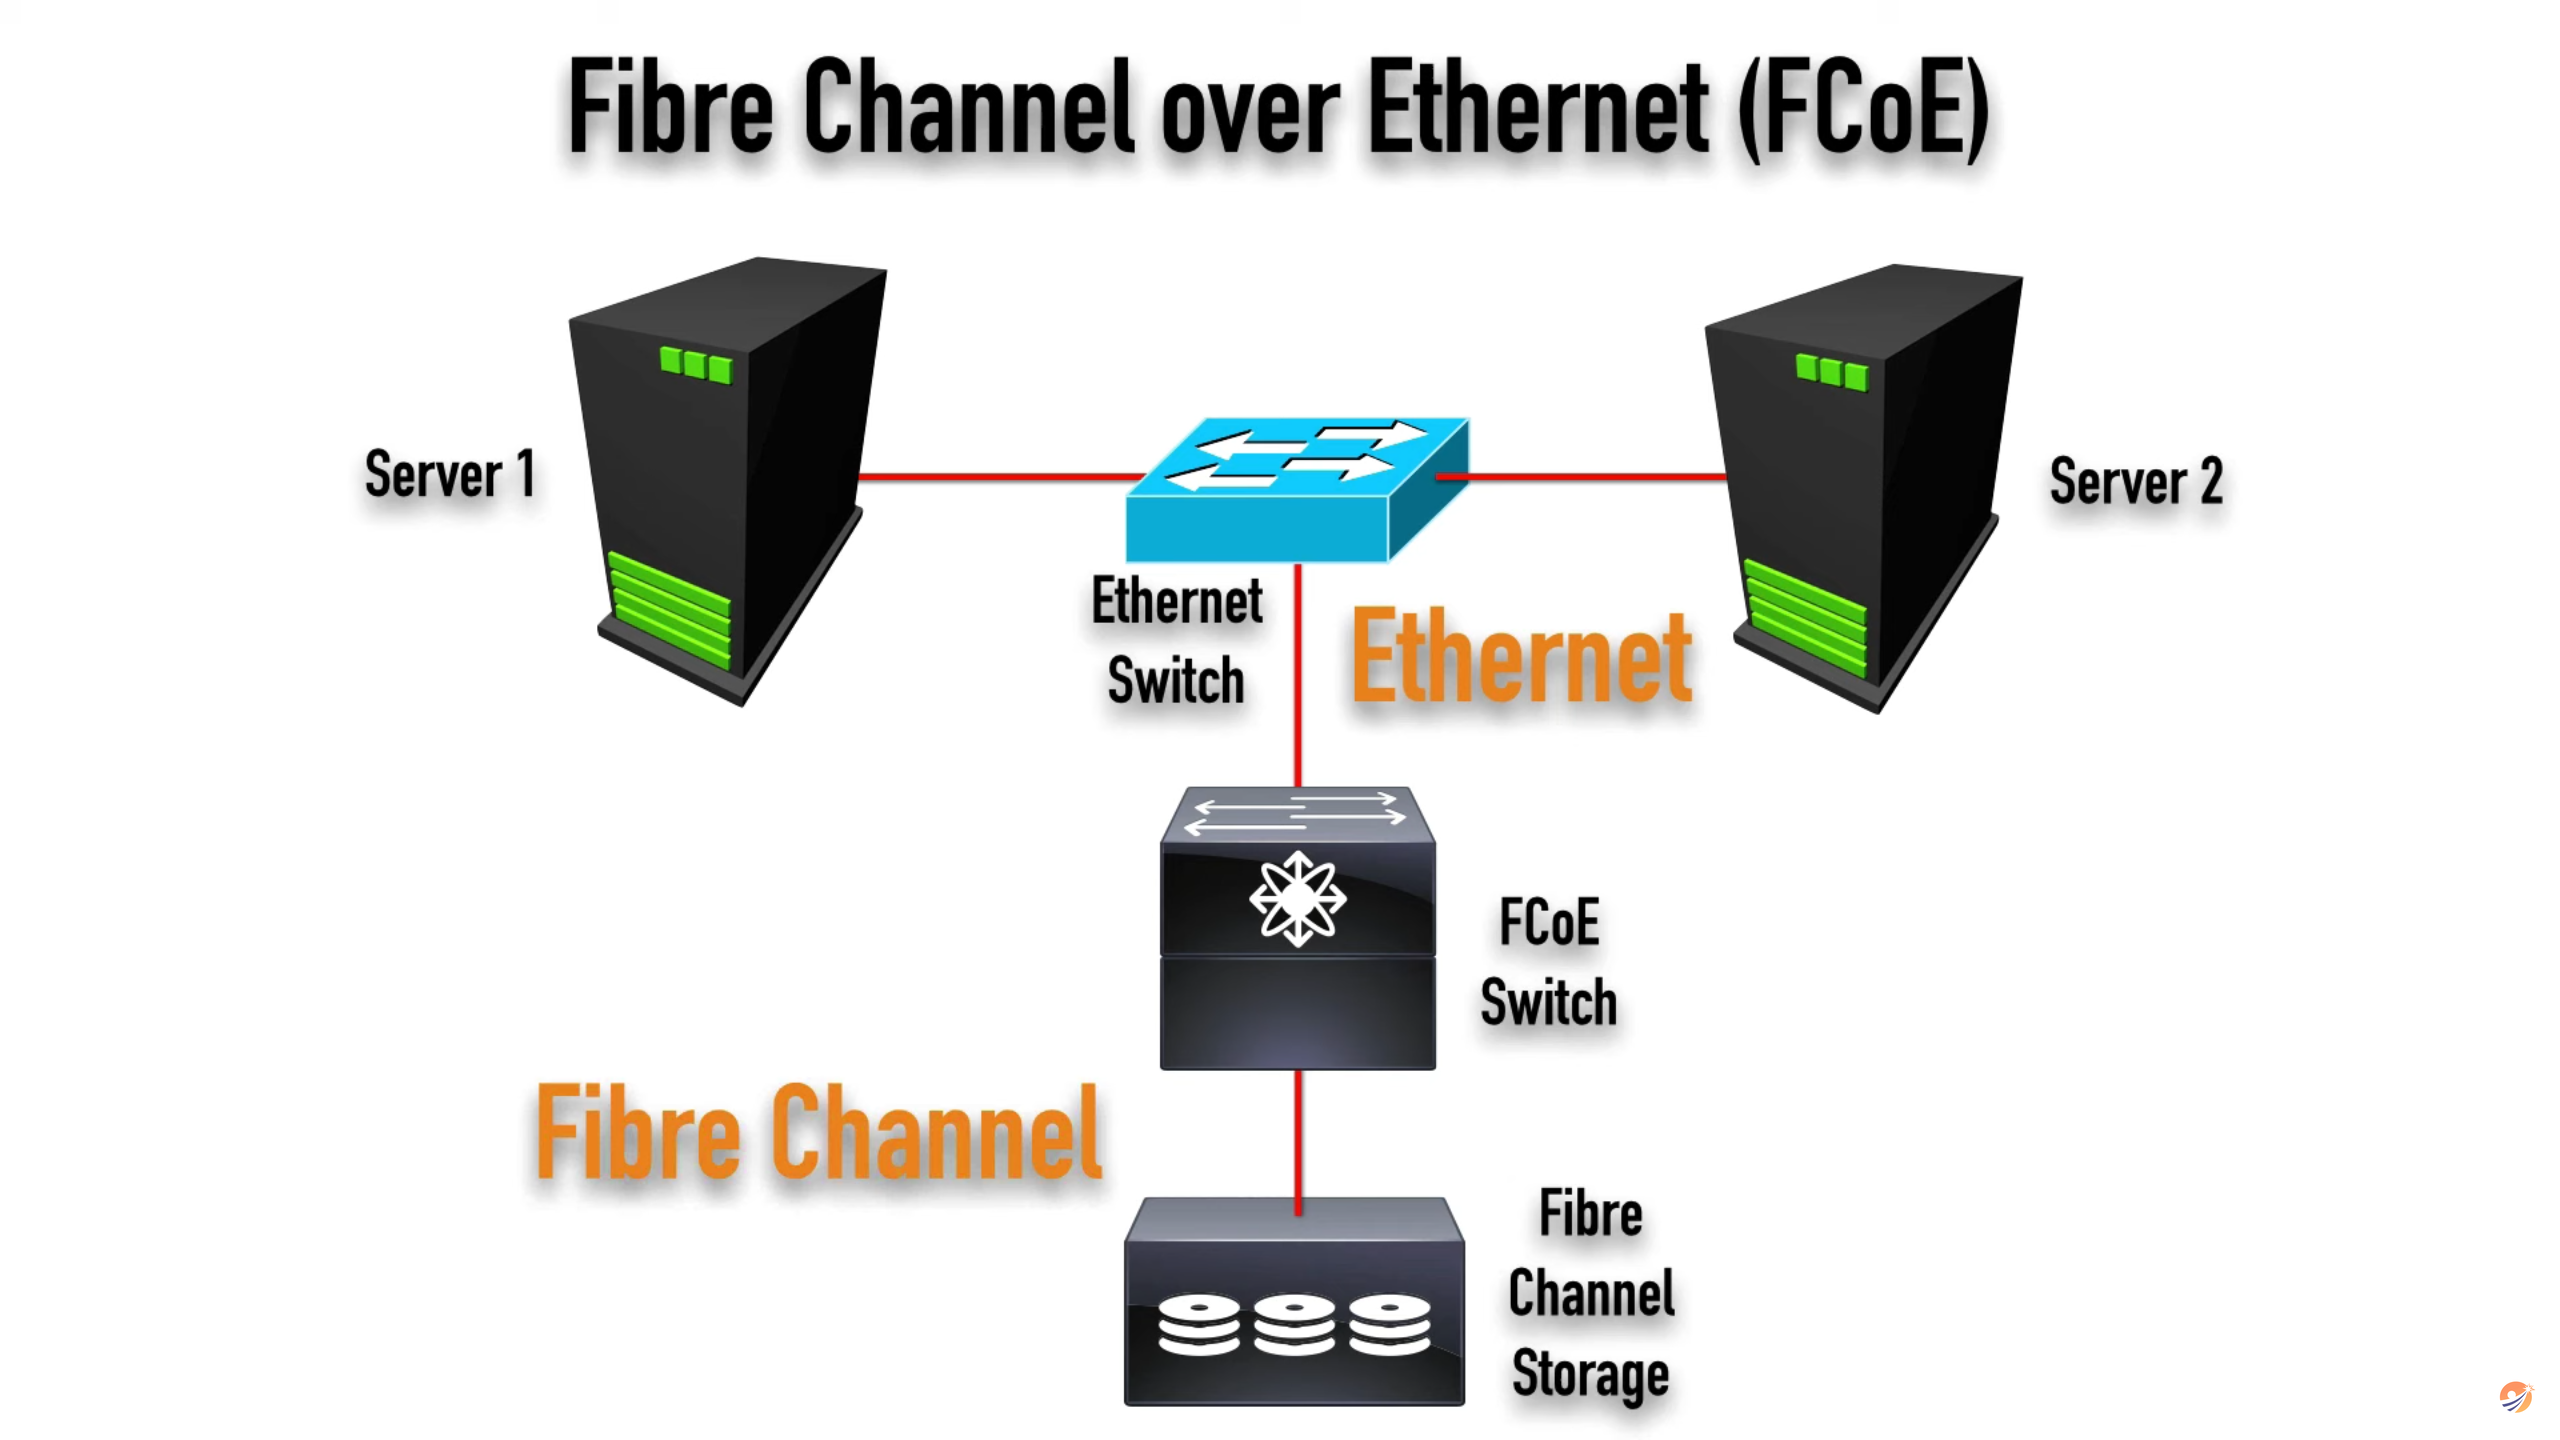
\includegraphics[width=0.32\columnwidth]{images/storage_fabric2.png}
   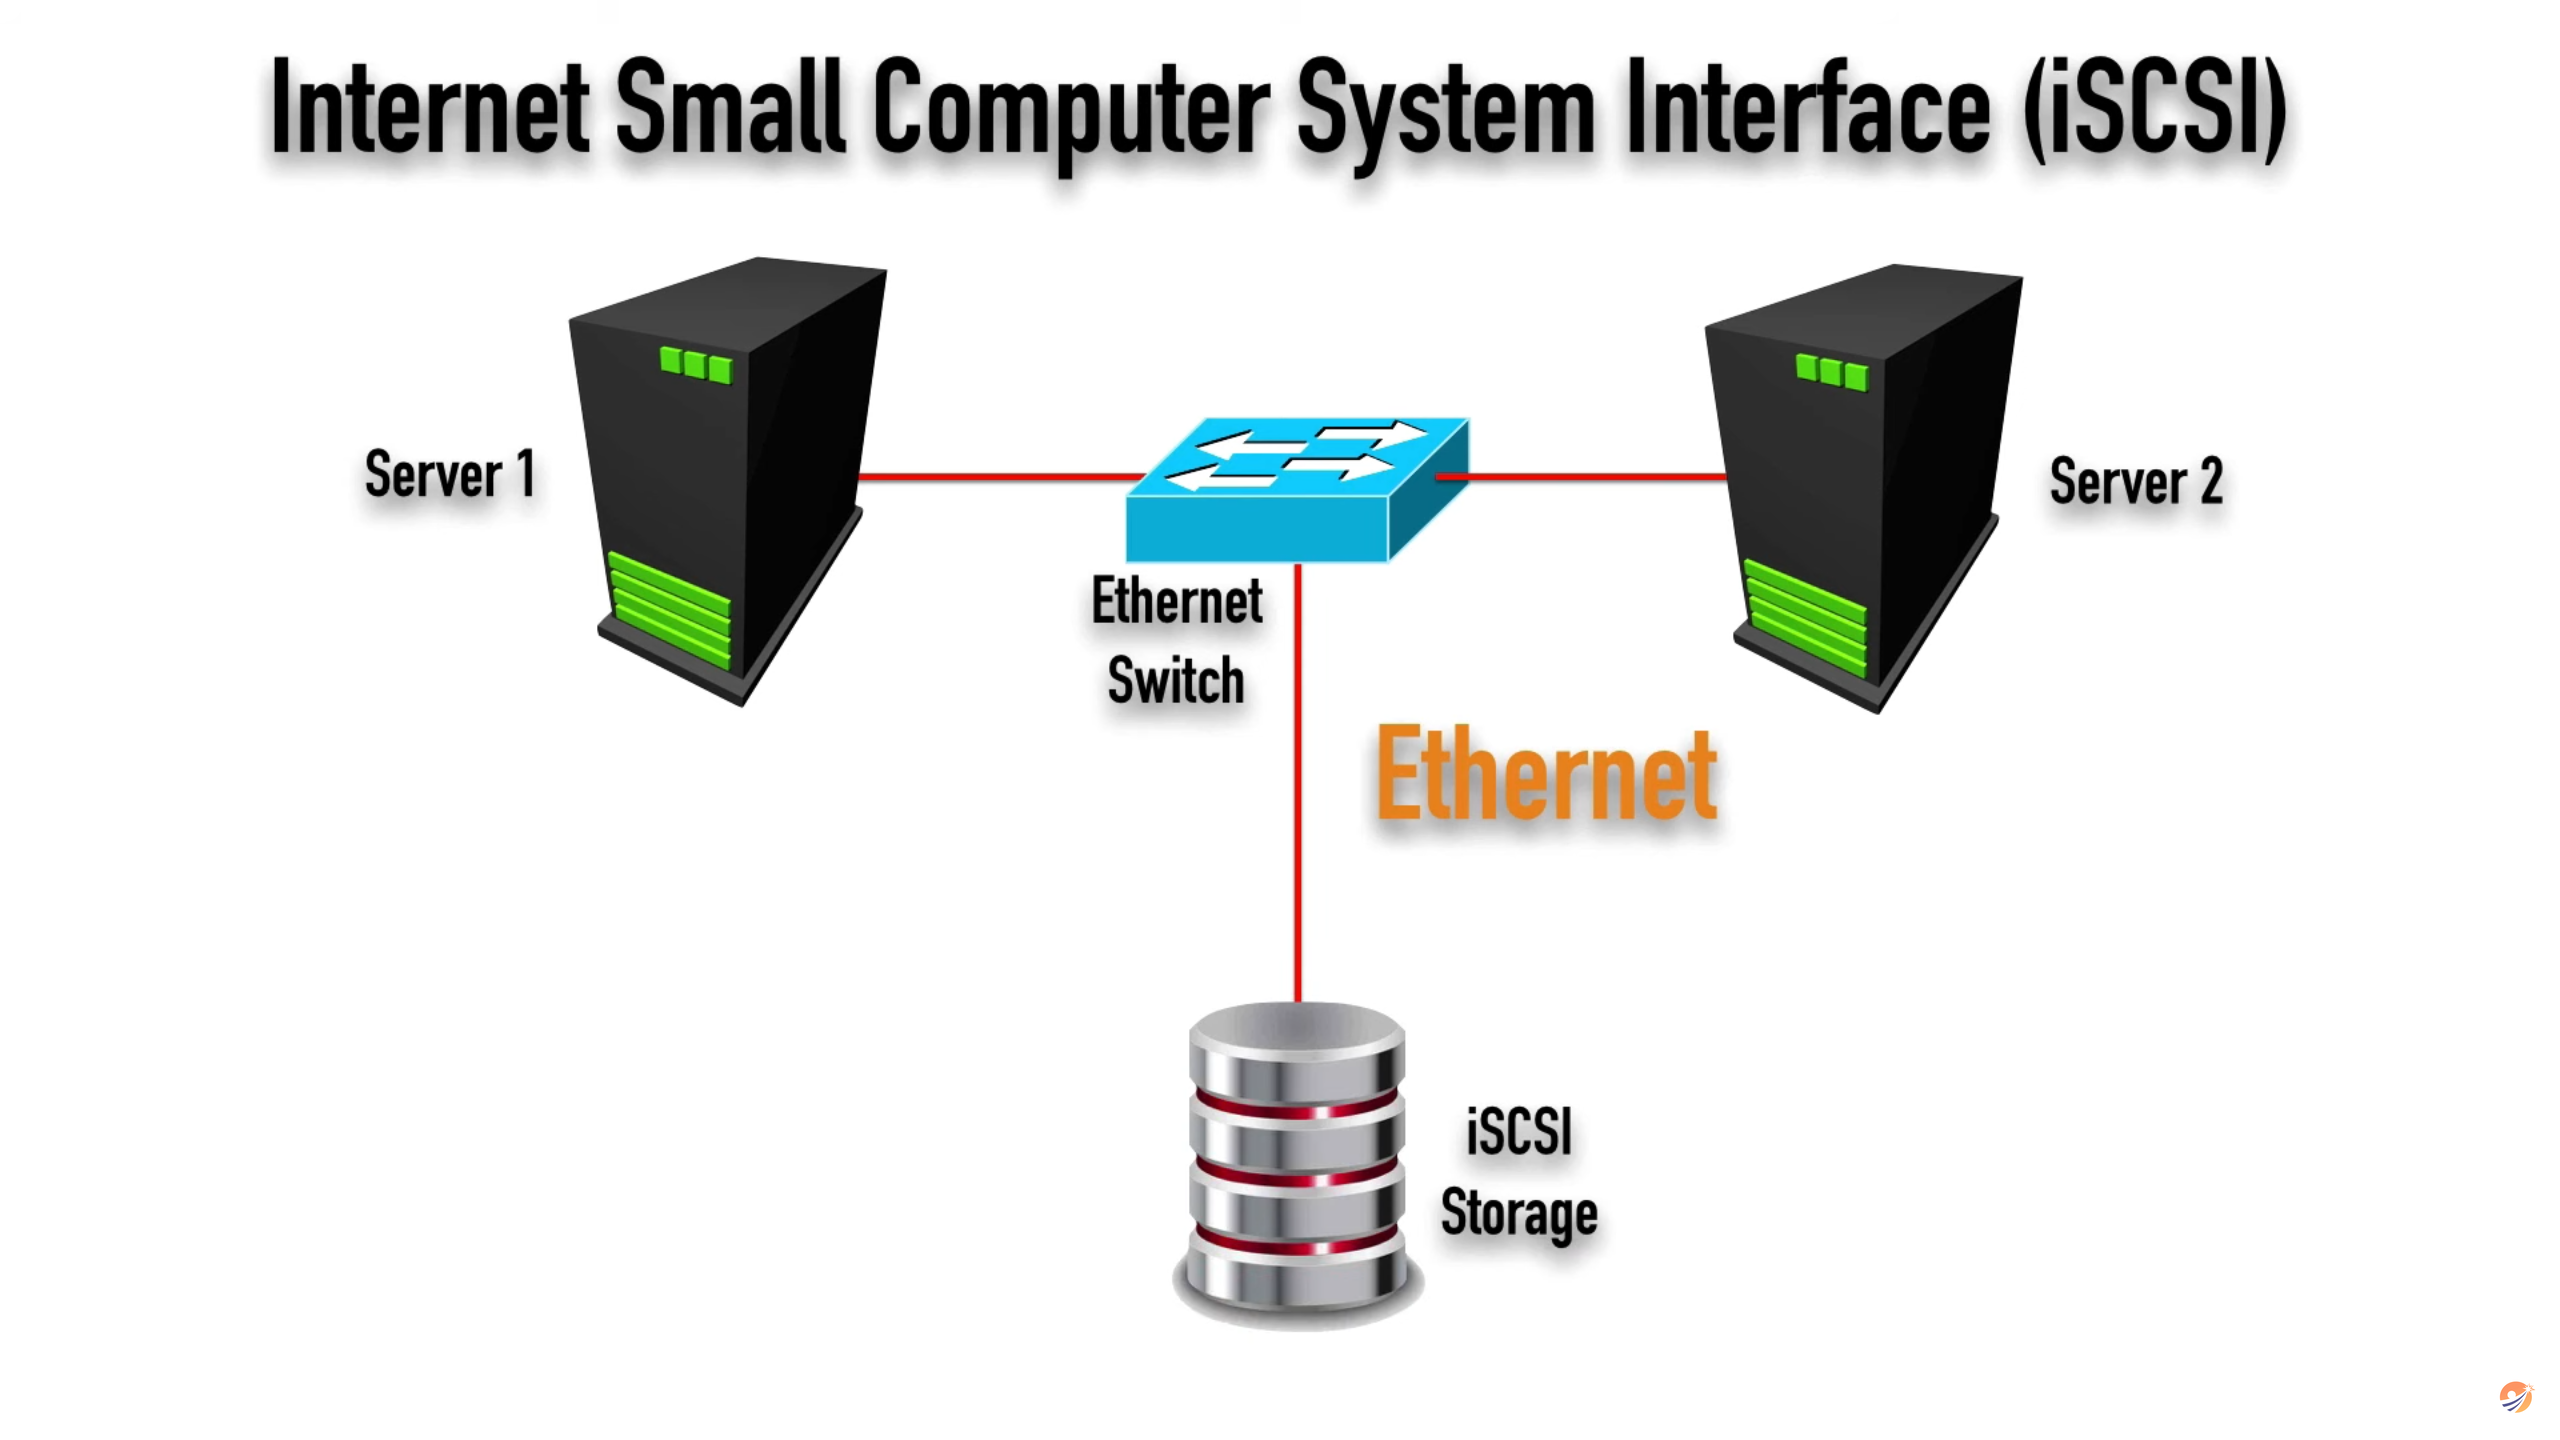
\includegraphics[width=0.32\columnwidth]{images/storage_fabric3.png}
   \caption{These are three possible configurations for the storage fabric, the first being the most performant, and the third being the cheapest.
   Note that in the second picture the first link is Ethernet and the second is Fibre Channel.}
   \label{fig:storage_fabric}
\end{figure}
Note that the image may me misleading, since there may be multiple FC switches (as partially depicted in Fig. \ref{fig:fibrechannel}) and multiple storage racks.
   
\subsection{Bus, controller and some numbers}
A bus is a component to whom multiple devices may be attached. It has a clock and some lanes, 16 in the case of PCI, each one providing almost 1GB bandwidth, summing up to $\sim 15GB$: 4 drives are enough to saturate a full PCI bus, or a 100Gbit link ($12.5GB/s$).;
in fact an NVMe SSD has a bandwidth of 3.5GB/s, hence $3.5\times 4 = 14GB/s \simeq 15GB/s$.\\
NVMe is often used in the lower memory tier of the RAM: its speed is only one order of magnitude less than RAM, but can provide high capacity without any problem.
It may represent a valid super-fast cache level for the RAM and hence started being associated in one single level to implement a big RAM tier, in a totally transparent way for the system.

Since the software latency in disk IOs is 5 microseconds more or less,
TCP/IP software introduces also a latency of 70-80 microseconds, the disk is
no more a problem. Indeed, the problem is now the network, not only for the
latency, but also for the bandwidth: as stated before 4 NVMe totally saturate a 100 Gbps
link.

\section{Redundancy and backup}
\subsection{Checkpoints}
It's unpractical for a system to go down after 5 months. For this reason it is necessary to have \ul{\textit{checkpoints}, which are points in time where the system can be restored to.} The system can be restored to the last checkpoint, and the data that was written after the checkpoint can be re-applied. This is similar to what happens to applications on smartphones are closed and then re-opened, the application is restored to the last checkpoint.

\subsection{RAID}
\textbf{RAID} stands for \textit{Redundant Array of Independent Disks}. It is a technology that allows to combine multiple disks into a single logical unit, in order to increase the performance, the reliability, or both. There are different levels of RAID, each with different characteristics.

Historically \textit{Redundant Array of Inexpensive Disks}, because it was more common for disks to eventually fail, so RAID was the only countermeasure to this. Today, disks are more reliable, so RAID is used more for performance reasons.

In RAID, \textbf{XOR} is used to calculate the parity of the data. The parity is used to recover the data in case of a disk failure. The parity is calculated by XORing the data of the disks. The parity is stored on a separate disk, called the parity disk. The parity disk is used to recover the data in case of a disk failure.


\section{Network sharing architectures}
Before going into the details of the architectures, it is important to understand the difference between \textbf{protocols} and \textbf{architectures}.\\
\textbf{SMB/CIFS} is a protocol that allows to share files over the network. It is used by Windows, but it is also supported by Linux and MacOS. NFS is a protocol that allows to share files over the network, it is used by Linux and MacOS, but it is also supported by Windows.\\
NFS is faster than SMB, but it is also less secure. SMB is slower than NFS, but it is also more secure.\\
These however are protocols for file sharing, not properly ``architectures''.

\framedt{Capacity and system architecture}{
   When we talk about \textbf{capacity}, there are two measures which we can refer to:
   \begin{enumerate}
      \item \textit{Scale-\textbf{up}}:
      adding more disks to the same server
      \item \textit{Scale-\textbf{out}}:
      adding more servers to the same network
   \end{enumerate}
}

\subsection{File based - NAS}
\textbf{NAS} are devices that are connected to the network, and that are used to store files, providing aggregated capacity. They are used to store files that are accessed by multiple users, and that need to be accessed from multiple devices.
NAS systems have integrated HW and SW component, including CPU, memory, NICs, optimized OS for file serving, file sharing protocols and so on.\\
Typically they exploit SMB/CIFS or NFS protocols, or AFP over optical fiber, and represent a good solution for \textit{document management}.

\subsection{Block based - SAN}
\textbf{SAN} stands for \textit{Storage Area Network}, which enables the creation and assignment (i.e. access and share) of storage volumes to compute systems.\\
The compute OS (or hypervisor) discovers these storage volumes as local drives.
The servers have different NICs (HBA) connected (usually through
fibre channels) to those blocks, which are aggregated volumes.\\
SAN also enables performance optimization of the storage by performing
deduplication (delete sequence of blocks that are equivalent).

\note{HBA stands for \textit{Host Bus Adapter}, and is a device that allows to connect a computer to a storage device. It is used to connect a computer to a storage device, and to allow the computer to access the storage device.}

SAN are a network separate from the LAN, so not affected by its traffic.\\
They usually exploit Fibre Channel or iSCSI (which is not as fast) protocols.

SAN was, before SSDs, one of the datacenter pillars.
Its architecture included a ``head'', an advanced Fibre Channel switch, to which drives were attached, and the head was connected to the network. The head was used to manage the drives, and to allow the servers to access the drives.\\
When SSDs became popular, the head became a bottleneck, because it was not able to keep up with the speed of the SSDs(Recall that 4 SSDs are enough to saturate a 10Gbit link, See Sec. \ref{sec:bandwidth_storage}). 
For this reason, the head may be removed, with the drives connected directly to the servers. This is called \textbf{DAS}, typically uses SCSI protocol, but is not as scalable as SAN.

However with groups of mechanical drives, ---if the data is splitted in a smart way--- it's possible to be faster of a single SSD, since the request will be forwarded in parallel to different drives.

\subsubsection{Protocols}
SANs are classified based on protocols and fabric they support. Some possible configurations can be found in Fig. \ref{fig:storage_fabric} 
Common SAN deployments types are Fibre Channel SAN (FC SAN), Internet Protocol SAN (IP SAN), and Fibre Channel over Ethernet SAN (FCoE SAN), ATA over Ethernet (AoE) and HyperSCSI ().
It can be implemented as some controllers attached to some JBoDS (Just a Bunch of Disks).

\note{While NAS provides both storage and a file system, SAN provides only block-based storage and leaves file system concerns on the “client” side.
However, note that a NAS \textit{can} be part of a SAN network.}


\subsubsection{Pools and LUNs}

\textbf{Storage pools} are used to combine multiple storage devices into a single logical unit, in order to increase performance and reliability. 

The SAN is divided in different Logical Unit Numbers (\textbf{LUN}s), which abstract identity and internal functions of storage devices, and appear as phyisical storage to the compute system.\\
\textbf{Storage LUNs} define a storage partition and are used to assign storage ---a portion of the pool--- to a server, and to allow the server to access the storage, using ACLs.
\nl

In the following section, some LUNs features are listed
\begin{itemize}
   \item 
   Storage \textbf{capacity} of a LUN can be dynamically expanded or reduced
   by means \textbf{virtual storage provisioning}, i.e. present a LUN as if it has more capacity than it actually has, to avoid fragmentatation and then expand it when it is needed.
   \note{e.g. if you assign a 1TB LUN to a server, and then you need to expand the LUN due to lack of space, if you have space next to the already assigned TB you can avoid fragmentation. Besides, if you can put data in only 1TB instead of 2TB (even if you present the volume as if it had 2TB), internal fragmentation may happen only inside that TB, and later on you can expand the volume up to the reserved 2TB.}
   Besides, \ul{available space may \textit{decrease} over time}, mostly due to snapshots (discussed later on).
   \item LUNs may perform \textbf{deduplication} (delete sequence of blocks that are equivalent/redundant, and exploiting indexes to retrieve duplicated data) to optimize storage performance. It is very useful in document-rich file systems, since people tend to copy a document multiple times.
   \item LUNs may perform \textbf{compression} to reduce the size of the data, and to increase the performance. It may be lossy or lossless.  Its major downside is that it is computationally expensive, since the data must decompressed before using it.
   On the other hand, allows to spare bandwidth by sending compressed data, which we know to be critical.\\
   \textit{Searching} in compressed data is not trivial, but there are tools to do it, such as the \href{https://en.wikipedia.org/wiki/FM-index}{\texttt{FM-index}}.
   \item LUNs may create \textbf{snapshots}, \textit{``point-in-time''} copy of current data state, to save the differences between the current state of the data and the previous state of the data. This allows to recover the overwritten data in case of a failure, but it also takes up space.\\
   Snapshots older than a week are usually deleted, since they are not needed anymore.
   
\end{itemize}

\subsubsection{Provisioning and Capacities}
LUNs may be created from\ns
\begin{itemize}
   \item A \ul{RAID set} (traditional approach); suited for application that require predictable performance
   \item A \ul{storage pool} (modern approach); suited for application that require flexibility and scalability, and that tolerate performance variations.
\end{itemize}

Both of these approaches have different capacities:\ns
\begin{itemize}
   \item Row capacity: the total capacity of the LUN, limited by the physical capacity of the storage devices
   \item Usable capacity: the capacity that is available to the server, limited by data structures needed to allocate the file system.
   \item Provisioned capacity: the capacity that you present to the server. May be more than the usable capacity, obtaining overprovisioning. 
\end{itemize}

\subsection{Object based - S3}
\textbf{S3} stands for \textit{Simple Storage Service}, and is a service that is used to store file data in the form of objects based on the content and other attributes of the data rather than the name and location of the file.
The additional metadata (size, date, ownership\dots) or attributes (retention, access pattern\dots) enable optimized search, retention and deletion of objects.\\
A flat, non-hierarchical address space to store data provides the flexibility to \textit{scale massively}.\\
\ul{S3 is leveraged to provide Storage as Service.}

\subsection{Big Data - HDFS}
\textbf{HDFS} stands for \textit{Hadoop Distributed File System}, and is a distributed file system that is used to store large amounts of data across multiple servers.
A \texttt{map/reduce} algorithm is applied on the data, and then results are collected and summarized.\\
It exploits good forms of parallelism to run efficiently the algorithm

\subsection{Unified - Unified Storage}
\textbf{Unified Storage} or multi-protocol storage has emerged as solution that consolidates block, file and object storage into a single storage platform. It supports multiple protocols, such as NFS, SMB, iSCSI, FC, REST and SOAP.

\framedt{iSCSI and its death}{
   SCSI (Small Computer System Interface) was invented in 1979 for chaining drives
   through a bus (used for e.g. in fibre channels). The controller was so smart
   to allow the the drive to share the flat cable as a bus.\\
   Over the time some variants were invented, but the basic idea is the same.
   One example is iSCSI: \textit{Internet Small Computer Systems Interface}, an IP-based storage networking standard for linking data storage facilities.
   It provides block-level access to storage devices by carrying SCSI commands over a TCP/IP network. The protocol died when SSD were introduced, since the latency was too high when communicating over the network.

   The key idea behind SCSI was for \ul{mutiple drives to share the same physical flat cable}.\\
   It had been ``deprecated'' in favor of \texttt{NVMe}, but it is still used today, because it is very reliable.
}
\subsection{Synchronization Software and its Price}
The ``storage guy'' must ensure that there is no condition under which can happen data loss, because it is never an option. It is also important to have powerful \textbf{synchronization algorithms}, which must allow data to be copied and synchronized in multiple locations without disrupting performance and handling concurrency;
such software is typically \textit{costful}.

It is difficult nowdays to establish what is the ``right'' price for software. The shift from highly specialized and costful hardware to general hardware-plus-software, gave the software, which still is a non-physical entity, increasingly more value, perhaps even too much.


\section{Hyperconverged Infrastructure}
SAN started to create a sensible bottleneck, so designers started to ``move drives towards the servers''.
\textbf{DAS} stands for \textit{Direct Attached Storage}, and is a technology that allows to connect multiple storage devices to a single server, in order to increase the performance, the reliability, or both.
The limitations is that you can only attach up to 2 or 3 drives to a server.

An idea came out to use the servers' internal drive to build a Storage Area Network, and this is called \textbf{VSAN}.

\subsection{HCI solutions}
\textbf{HCI} stands for \textit{Hyperconverged Infrastructure}, and is a technology that allows to combine multiple servers into a single logical unit, in order to increase the performance, the reliability, or both. 
The idea was born to allow a scale-out architecture, where you can add more servers to the network.

\begin{center}
   \ul{\textit{``Adding servers adds capacity''}}
\end{center}

The \textbf{Hypervisor} is the software that allows to run multiple virtual machines on a single server. There should be some locality between the VM and the storage, because the VM should be able to access the storage quickly.\\
The \textit{controller VM} (one per host) implements the storage abstraction and the logical moving of data.
\texttt{read} operations are always performed locally on local drives; \texttt{write} operations instead sometimes require to retrieve a remote piece of data.
A copy on the local server storage is kept, but the server needs to wait for the acknowledgment of the remote server in order to keep updated replicas of written data in other nodes.

As mentioned in the section dedicated to HCI and networking Sec. \ref{sec:HCI_network}, new server are automatically added to the network seamlessly integrating with the pre-existing HCI cluster.
The same applies to the storage, which is automatically added to the pool, and local replicas of data are built.

\subsubsection{VM Live Migration}
Live Migration of VMs is a technique that allows to move a VM from one server to another server, without interrupting the service. 
When it happens over SAN there's no need to copy storage to the new server, since the storage is shared and accessed through the network.
The case of HCI is similar since the storage is mostly shared, but there are also the above mentioned local copies of data, which may need to be updated. 

\subsection*{Riak and Acropolis}
Riak is a distributed database that is used to store data in multiple locations. 
The same applies to Acropolis, which is a distributed storage system.

Recently it has been recognized that \ul{using general purpose hardware is no longer a feasible option.}

\section{SDS - Software Defined Storage}
\textbf{SDS} \textit{Software Defined Storage} refers to software for policy-based provisioning and management of data storage independently from the underlying hardware.
Such software is more costful than the hardware it is running on, since it also optizimes the drives, not simply managing them.\\
SDS exploits object-based storage architecture and DHTs to provide storage services.
\chapter{Attacks}
% \section*{3 - Ottobre}
\section{Attacks and Vulnerabilities}
Following the discovery of a vulnerability $v$ there's an analysis to evaluate which attacks are enabled by $v$.
\textbf{Attacks} can be described as a set of attributes:
\begin{enumerate}
    \item Precondition
    \item Postcondition
    \item Success Probability
    \item Know how, abilities, tools required
    \item Noise = Probability of being discovered
    \item Automated/Potentially automatable/manual
    \item Local/Remote
    \item Actions to implement attack\footnote{See following Section on attack taxonomy}
\end{enumerate}
Even though some attack evaluation proposals map to each attribute a number and combine them into a value,
such evaluations do not consider that \textbf{risk} resides in \textit{intrusions}, not individual attacks, because they have a considerable impact on the system, and keep in mind that are composed by:
\begin{itemize}
    \item Exploration and information collection
    \item Persistence
    \item Attack \textit{chain} for privilege escalation
\end{itemize}

\section{Attack Classification}
\label{sec:attack_taxonomy}
The actions need to implement an attack may be used to define a \textbf{taxonomy} of attacks:
\begin{enumerate}
    \item buffer/stack/heap overflow
    \item \textit{sniffing} $\rightarrow$ Illegal access to info in travel
    \item \textit{replay attack} $\rightarrow$ Repeated exchange of legal messages 
    \item \textit{Interface attack} $\rightarrow$ Illegal order in the invocation of API functions
    \item \textit{Man-in-the-middle} $\rightarrow$ Interception and manipulation of info in travel
    \item Diversion of an information flow
    \item \textit{Race-condition} $\rightarrow$ Time-to-use time-to-check
    \item \textit{Cross site scripting} $\rightarrow$  XSS
    \item SQL injection
    \item \textit{Bell-Lapadula policy} $\rightarrow$ Covert channel 
    \item Masquerading as
    \begin{itemize}
        \item user
        \item machine (\textit{IP/DNS spoofing, Cache poisoning}
        \item connection (\textit{connection stealing/insertion})
    \end{itemize}
\end{enumerate}

\section{Examining attacks}
\subsection*{Replay attack}
Suppose a user asks the bank to transfer some money to $Y$ account with an $M$ message.
$Y$ may sniff and record $M$, and before the secure channel $S$ gets deleted, $Y$ sends $M$ several times.\\
Note that the attack may work even if encryption is used.

\subsection*{Man-in-the-middle}
If $A$ and $B$ communicate, $E$ may pose itself in the middle, acting as if it were $B$ to $A$ and $A$ to $B$.
Such attack is possible when no authentication is required.

\subsection*{XSS}
A website allows users to upload contents to be later (possibly) downloaded by users.
Thus a malicious user may upload hidden scripts to damage or steal information from the user who download their content.
To avoid this the website must check the content uploaded by users.\\
A well known attack of this type targeted BBC.

\subsection*{SQL Injection}
An input may insert a malicious query (i.e. \lstinline[language=SQL]{DROP TABLE USERS}) in a credentials field.
The best way to avoid this is to whitelist using RegEx.

\subsection*{Cryptography attacks}
These are a category on their own, there are many types, with different variations and features.

\subsection*{Side-channel attacks}
Any attack that measures some physical value to discover an encryption key.
Currently it is popular due to the capabilities of machine learning in exploiting large number of pairs to deduce a function.\\
Such measures may be:
\begin{itemize}
    \item Electromagnetic emissions
    \item Energy consumption
    \item Execution time to discover inner status
    \item Execetion time to discover cache usage and prediction mechanisms.
\end{itemize}

\subsection*{Virtual Machines \& Blue Pill}
Cyber system may be composed of many virtual machines onion-like organized.
Thus, attacking a low-level VM may grant access rights to higher ones.\\
Besides, an attacker may insert a new VM in the hierarchy:
this is called \textit{Blue Pill} attack, it's hard to discover and has a high impact.
A new VM may return to higher VMs fake information on the status of the underlying machines and/or send malicious commands to the underlying machines.\\
\texttt{Stuxnet} was a malware which used to send commands to uranium enrichment centrifuges to destroy them, and meanwhile told the operator that everything was going well.  

\chapter{Cloud computing}
\section*{19 - Ottobre}
Powerful hardware and high-speed networking have made room for the development of cloud computing.
\textbf{Cloud computing} allows virtual resources accessible \textbf{on demand},
and provides many advantages against the standard old-style scaling methods i.e. buying resources.
\begin{itemize}
   \item \textit{Scalability}
   \item \textit{Elasticity}
   \item \textit{Resilience}
   \item \textit{Cost}
\end{itemize}

\section{Virtualization and Containers}
\begin{paracol}{2}
   Virtual machines on a single physical machine are managed by hypervisor
   \begin{table}[!htbp]
      \centering
      \begin{tabular}{|cc|}
         \hline
         App A & App B\\
         bins/libs & bins/libs\\
         Guest OS & Guest OS\\
         \midrule
         \multicolumn{2}{|c|}{\textbf{Hypervisor}}\\
         \hline
         \multicolumn{2}{|c|}{Host OS}\\
         \hline
         \multicolumn{2}{|c|}{Hardware}\\
         \hline
      \end{tabular}
   
   \end{table}

   \vspace{\fill}
   \switchcolumn

   Containers instead exclude one layer of abstraction, saving up a lot of resources
   \vspace{\fill}
   \begin{table}[!htbp]
      \centering
      \begin{tabular}{|cc|}
         \hline
         App A & App B\\
         bins/libs & bins/libs\\
         \midrule
         \multicolumn{2}{|c|}{\textbf{Container Manager}}\\
         \hline
         \multicolumn{2}{|c|}{Host OS}\\
         \hline
         \multicolumn{2}{|c|}{Hardware}\\
         \hline
      \end{tabular}
   \end{table}

   \vspace{\fill}
\end{paracol}

\section{Docker}
Docker exploits container-based virtualization to run multiple isolated guest instances on the same SO.
Software is packaged into \textbf{images} which are read-only templates to instantiate and run containers.
External \textbf{volumes} can be mounted to ensure data persistance when used by multiple containers or by the host machine.

It is possible to \textbf{stack} multiple docker \textit{images},
and if desired create a new image as a result of stacking other ones.
\chapter{Containers}
\label{chap:containers}

\ul{A VM is better than a process because it provides \textbf{isolation}}:
a typical problem in cybersec is that if an attacker cracks a process, he may access the whole system;
with a VM, the attacker can only access the VM, not the host.
However, a VM introduces overhead due both to the hypervisor and to the OS (cache, kernel, storage management\dots).

\note{The idea is to tell a process that a process that its root is a subdirectory of the host's root, resulting in a strong isolation.}

\textbf{Docker} provides a \textit{differential filesystem}, which is a filesystem that is a diff of the host's filesystem, an abstraction where the new ``inner'' file system is based on a given one, where the system will only store the differences between the original file system and the new one.

Docker has become the de facto standard for containers, but there are other solutions like \textbf{LXC} (Linux Containers) and \textbf{rkt}.
A Dockerfile contains the information to build a container.

One of the key differences between a VM and a container is that containers \textbf{do \textit{not} have a virtual switch}.
A container uses the same MAC address of the host.\\
Docker containers are processes, and only see a portion of the host's filesystem.

Inside a Dockerfile you may create temporary containers by exploiting multiple images and lastly build the resulting slimmed image.

\section{Upgrading a system}

Typical procedure when a system needs to be updated: create first a snapshot before updating the containers (especially if there are updates related to the database), then update, run back the containers, check if everything works, and then delete the snapshot. If anything goes wrong, the snapshot will help to roll back.

\section{Docker compose}
Docker compose is a tool to define and run multi-container Docker applications. It uses a YAML file to configure the application's services, networks and volumes. With a single command, you can create and start all the services from your configuration.

Kubernetes is a more advanced tool for container orchestration, way more complex than Docker compose, it allows to manage thousands of containers, providing fundamental scalability features.

\section{Docker security}
An attack is to put the machine under heavy workload and observe from the container the performance to infer what other processes may be. This is called \textbf{side channel attack}.

Google has thousands of VMs and each runs a \textit{container for each query}.
\chapter{Cloud}
Cloud came out as a business model, not as a technlogy.
It was needed to handle peak of requests and to allow scalability, without oversizing Infrastructures.
\note{e.g. Amazon needs to handle way more requests on Christmas than on a normal day.}
So, Cloud was a mean to reduce the cost of the ICT infrastructure.

\textbf{Resource pooling} is the key concept of Cloud. It means that the services are provided to users using a multi-tenant model, with physical and virtual resources being dynamically allocated and deallocated according to the demand.\\
Cloud was needed also to provide rapid elasticity, meaning that capabilities may be elastically provisioned and released, in some cases automatically, to scale rapidly outward and inward commensurate with demand. To the customer it means that the capabilities available for provisioning often appear to be unlimited and can be appropriated in any quantity at any time.

Benefits of Cloud:
\begin{itemize}
   \item \textbf{Business agility}
   \begin{itemize}
      \item Quick resource provisioning
      \item Facilitates innovation
      \item Reduces time to market
   \end{itemize}
   \item \textbf{Reduces IT costs}
   \begin{itemize}
      \item Reduces up-front capital expenditure (CAPEX)
      \item Improves resource utilization
      \item Reduces operational expenditure (OPEX)
   \end{itemize}
   \item \textbf{High availability}
   \begin{itemize}
      \item Ensure resource availability based on customer's requirements
      \note{In RAI, prof. Cisternino experienced people complaining because their servers' CPUs were running at 98\% of their capability, and they wanted to exploit also the remaining 2\%, because ``they paid for it''.}
      \item Enables fault tolerance
      \note{Recall active-active, active-passive, etc. configurations.}
   \end{itemize}
   \item \textbf{Business continuity}
   \item \textbf{Flexible Scaling}
   \item \textbf{Flexibility of Access}
   \item \textbf{Application Dev and Testing}
   \item \textbf{Simplified infrastructure management}
   \item \textbf{Increased collaboration}
   \item \textbf{Masked complexity}
\end{itemize}
Cloud has the magic power of decoupling the software from the hardware.

Disadvantages of Cloud:
\begin{itemize}
   \item Vendor lock-in
   \item Privacy
   \item Your software depends on someone else
   \item Legislation is complicated
   \note{In EU public administration data, must be stored in the EU.}
   \item \dots TODO
\end{itemize}

\section{Cloud Service Models}
\begin{itemize}
   \item \textbf{IaaS} (Infrastructure as a Service)
   \begin{itemize}
      \item Provides virtualized computing resources over the Internet
      \item Examples: Amazon EC2, Google Compute Engine, Microsoft Azure
   \end{itemize}
   \item \textbf{PaaS} (Platform as a Service)
   \begin{itemize}
      \item Provides a platform allowing customers to develop, run, and manage applications without the complexity of building and maintaining the infrastructure
      \item Examples: Google App Engine, Microsoft Azure, Heroku
   \end{itemize}
   \item \textbf{SaaS} (Software as a Service)
   \begin{itemize}
      \item Provides software applications over the Internet
      \item Examples: Google Apps, Microsoft Office 365, Salesforce
   \end{itemize}

\section{Cloud Deployment Models}
\begin{itemize}
   \item \textbf{Public Cloud}
   \begin{itemize}
      \item Owned and operated by third-party cloud service providers
      \item Deliver computing resources over the Internet
      \item Examples: Amazon Web Services (AWS), Microsoft Azure, Google Cloud Platform
   \end{itemize}
   \note{It does \textbf{not} mean that the data is public. It means that the cloud services are accessible to the public.}
   \item \textbf{Private Cloud}
   \begin{itemize}
      \item Operated solely for a single organization
      \item Managed by the organization or a third party
      \item \textit{On-premise} or \textit{off-premise}
   \end{itemize}
   \note{It does \textbf{not} mean that the data is private. It means that the cloud services are accessible only to the organization e.g. \textit{UniPi}.}
   \item \textbf{Hybrid Cloud}
   \begin{itemize}
      \item Composition of two or more clouds (private, community, or public) that remain unique entities but are bound together, and resources may be moved from one cloud to another (with some performance cost obviously) 
      \item By standardized or proprietary technology that enables data and application portability
   \end{itemize}
   \item \textbf{Community Cloud}
   \begin{itemize}
      \item Shared infrastructure for specific community
      \item Managed by organizations or third party
      \item On-premises or off-premises
   \end{itemize}
\chapter{Deception with Honeypots}
A \textbf{honeypot} is a system designed exclusively to be attacked an to \textbf{collect information} about the attacker and its tactics, techniques and procedures;
the other focus of an honeypot is also to possibly slow down an attack to a system by \textbf{diverting} it on itself.

The scaled version of a honeypot, is a \textbf{honeynet},
which is an entire network attached to a real system designed to be targeted instead of the main system.

\subsection{Classification}
\begin{enumerate}
   \item \textbf{Interaction}-based
   \begin{enumerate}
      \item \textit{Low} - e.g. simple port listener
      \item \textit{Medium} - emulation of a network service that analyzes the inputs and returns some replies similar to those the real service would return.
      \begin{itemize}
         \item Simulates just some \textbf{features} of the service
         \item Easy to implement, \textbf{low risk}
         \item Can collect a low amount of information
         \item Tools $\longrightarrow$ OS + Honeyd
      \end{itemize}
      \item \textit{High} - built around real services that run on real machines to fool the attacker
      \note{realistic but dangerous due to the large amount of vulnerable software}
      \begin{itemize}
         \item Simulates \textbf{all features} of the service and of the underlyng OS
         \item The attacker may fully compromise and control it
         \item \textbf{High risk}
         \item A larger amount of information
         \item Tools $\longrightarrow$ Honeynet.
      \end{itemize}
   \end{enumerate}
   
   \item \textbf{Implementation}-based
   \begin{enumerate}
      \item \textit{Virtual}
      \item \textit{Physical}
   \end{enumerate}
   
   \item \textbf{Goal}-based
   \begin{enumerate}
      \item Production
      \item Research on attacker behaviour
   \end{enumerate}
\end{enumerate}

\section{Honeyd}
\textbf{Honeyd} is a daemon which creates virtual nodes in a network.
It is highly configurable and is able to reproduce even large and complex networks;
besides it can integrate with virtual and physical real-existing networks.\\
\textbf{Honeyd} provides many features, we can list some of the main ones:
\begin{itemize}
   \item It detects illegal activities in a network by monitoring the IP addresses that are not within a \textbf{range} named \textit{"dark space"}.
   Any attempt of connection to or from the \textit{dark space} is assumed to be an attack or a vulnerability scan.
   \item It monitors activities related to TCP and UDP ports and ICMP traffic.
   \item It can emulate network services using script in Perl, shell or other way of interacting with the attacker.
\end{itemize}

\subsection{Architecture}
\begin{itemize}
   \item \textit{Configuration database} -
   Queried to discover the model paired with the destination IP address
   \item \textit{Packet dispatcher} -
   analyzes input packets and checks correctness and integrity.
   Anything different from TCP, UDP and ICMP gets \textit{discarded}.
   \item \textit{Protocol manager} -

   \item \textit{Personality engine} -
   computes a reply packet and updates it to guarantee coherence with the OS that the destination is expected to use
   \item \textit{Optional routing component} -
   allows the routing of a packet to a real application
\end{itemize}

\subsection{Research results}
\textbf{Honeypot}s provided an important amount of data to perform research on.
Many statistics have been computed to produce estimations and interesting results,
a \textit{\textbf{UniPi} student presented a thesis on the topic} \smiley.
\note{Honeypot thesis available in the \href{https://elearning.di.unipi.it/mod/resource/view.php?id=18233}{web page of the course}}
\chapter{Partitioning}

\textbf{Partitioning} becomes necessary when dealing with \textbf{large data sets} and high \textbf{query throughput}. It is a technique that divides a large data set into smaller, more manageable parts. This is done to improve the performance of the system. Partitioning can be done in various ways, such as horizontal partitioning, vertical partitioning, and functional partitioning. In this chapter, we will discuss the different types of partitioning and their benefits.

``Partition'' is the most common term, but it may vary depending on the technology:
\begin{itemize}
   \item \textbf{Shard} in MongoDB, Elasticsearch, and Cassandra.
   \item \textbf{Region} in HBase.
   \item \textbf{VBucket} in Couchbase.
   \item \textbf{Tablet} in Bigtable.
   \item \textbf{VNode} in Riak and Cassandra.	
\end{itemize} 

\section{Partitioning concepts}
First, partitions must be \textbf{defined}, in the sense that each piece of data must be assigned to a partition. This can be done in various ways, such as hashing, range partitioning, or list partitioning.

Then, each partition should have its own \textbf{characteristics}, i.e. should support a known set of operations, since it acts as a small per se database.

Clearly, different partitions may reside on different nodes, enabling scalability.


\subsection{Combining partitioning with replication}

\begin{paracol}{2}
   \colfill
   Partitioning can be combined with replication to improve the performance and reliability of the system. Replication is the process of creating multiple copies of the data and storing them on different nodes. This ensures that the data is available even if one of the nodes fails. \ul{By combining partitioning with replication, you can achieve high availability and fault tolerance.}
   \colfill
   
   \switchcolumn

   \begin{figure}[htbp]
      \centering
      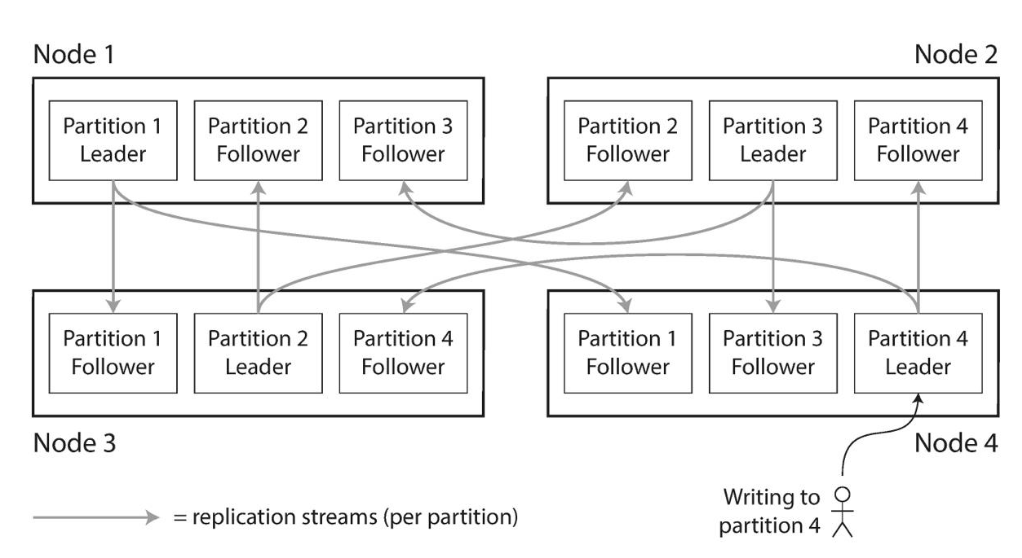
\includegraphics[width=0.95\columnwidth]{images/11/leader_follower.png}
      \caption{Leader-follower model}
      \label{fig:11/leader_follower}
   \end{figure}
\end{paracol}

This can be achieved in various ways:
\begin{enumerate}
   \item Node Storage of Multiple Partitions
   \begin{itemize}
      \item Nodes can store more than one partition, and \ul{each partition can be stored on multiple nodes}.
   \end{itemize}
   \item \textbf{Leader} and \textbf{Follower} assignment
   \begin{itemize}
      \item Each node stores a partition, and one of the nodes is designated as the leader. The leader is responsible for handling all write operations, while the followers replicate the data from the leader.
   \end{itemize}
   \item Replication and Partitioning
   \begin{itemize}
      \item The two techniques are enforced independently.
   \end{itemize}
\end{enumerate}

The Goal of partitioning is to spread data and query load \textbf{evenly} among the nodes.
Unfair partitioning can lead to \textbf{hot spots}, where some nodes are overloaded while others are underutilized.\\
Randomizing the partitioning function can help to avoid hot spots, but it can also make it difficult to locate data, requiring to query all nodes to get a value.

\subsection{Key-Range Partitioning}
A first improvement might be to provide a range-key assignment allowing to locate data, as it happens in libraries, where books are ordered by author or title.\\
In this way you know the boundaries of where to search. This is very easy to implement and to understand,
however, it is \textit{not} optimal:
\ul{data may \textbf{not} be evenly distributed among the possible keys}.

\section{Avoiding Hot spots}
So with key-range partitioning, the problem is that some keys may be more popular than others due to access patterns, leading to hot spots.\\
In, for instance, a sensor database, all today's writes would end up in the same ``today's partition'', while the rest of the partitions would be idle.
\nl

A solution might be to change-key structure, for instance by adding a prefix to the key, such as the sensor ID, to distribute the data more evenly.

\subsection{Hash partitioning}
A better solution is to use \textbf{hash partitioning}, where a hash function is used to map keys to partitions.\\
However we must be careful because \textbf{inconsistent} hashing can lead to hot spots, as the hash function may not distribute keys evenly.

Note also that hash partitioning is very bad for range queries, as even similar data is spread randomly across the partitions.

\subsubsection{Secondary Indexes}
% Copilot generated
Secondary indexes are a way to avoid hot spots in hash partitioning.\\
The idea is to create a separate index that maps the secondary key to the primary key, and then use the primary key to locate the data.\\
This way, the secondary key is hashed and distributed evenly across the partitions, while the primary key is used to locate the data.


\begin{itemize}
   \item \textbf{Document}-based partitioning (local indexes)
   \begin{itemize}
      \item Each listing has a unique document ID
      \item Database is partitioned based on the document ID
      \item Secondary indexes are on fields like color and make
      \item \ul{\textit{Reading} requires querying all partitions}
   \end{itemize}
   \item \textbf{Term}-based partitioning (global indexes)
   \begin{itemize}
      \item A Global index covers data in all partitions.
      \item Partitioning is based on the term ID, which is not the primary key index.
      \item 
   \end{itemize}
\end{itemize}

\section{Rebalancing}
Rebalancing is the process of moving data between partitions to ensure that the data is evenly distributed among the nodes. This is necessary when the data distribution changes, for example, when new nodes are added to the system or when the data distribution becomes uneven due to hot spots. Rebalancing can be done in various ways, such as automatic rebalancing, manual rebalancing, and dynamic rebalancing.

\framedt{Challenges in rebalancing}{
   \begin{itemize}
      \item Fair load distribution
      \item Continuous operation during rebalancing
      \item Minimizing data movement
   \end{itemize}
}

\subsection{Optimizing rebalancing - Kademlia and P2P recalls}

Assigning keys to nodes computing $h(key) mod \#{nodes} \rightarrow node$ is intuitive but leads to a tremendous amount of data movement when nodes are added or removed, since all modulo values must be recomputed.\\
A better solution is to use a \textbf{distributed hash table} (DHT) such as \textbf{Kademlia} or \textbf{Chord}, which allows to find the node responsible for a key in $O(\log n)$ steps.

A simple intuition exploited by both Kademlia and Chord is to fix the granularity of the keyspace prior to partitioning.

In other words, having a fixed number of partitions may help to avoid data movement when nodes are added or removed.


\subsection{Dynamic partitioning}
Dynamic partitioning is a technique that allows the system to adapt to changes in the data distribution. This is done by monitoring the data distribution and rebalancing the data when necessary. Dynamic partitioning can be done in various ways, such as automatic rebalancing, manual rebalancing, and dynamic rebalancing.

\begin{itemize}
   \item \textbf{Automatic} rebalancing - System automatically rebalances the data when necessary without any human intervention.
   May be unpredictable and expensive, but requires less maintanance.
   \item \textbf{Manual} rebalancing - Administrator manually rebalances the data when necessary. May be better since and admin may have a more \textit{comprehensive} view of the distributed system, while a machine may be limited by network partitioning, discovery, etc.
   \item \textbf{Hybrid} approach - Combines automatic and manual rebalancing. The system automatically rebalances the data when necessary, but the administrator can override the system's decisions. 
\end{itemize}

\subsection{Routing}
Routing is the process of determining which partition to send a query to. This is done by either forwarding requests to a routing tier, or by having partition-aware clients which know how the data is distributed. Routing can be done in various ways, such as static routing, dynamic routing, and consistent hashing.



The opposite approach is to query all partitions, which is very expensive, but may be necessary in some cases.


\section{Takeaways}
Data partitioning enhances scalability by distributing data across multiple nodes, and when combined with replication, it can improve the performance and reliability of the system. However, partitioning can introduce challenges such as hot spots and rebalancing. To address these challenges, you can use techniques such as hash partitioning, secondary indexes, and dynamic partitioning. By carefully designing the partitioning strategy, you can achieve high availability, fault tolerance, and scalability in your system.
\chapter{Transactions}

\begin{definition}
   [Transaction]
   A \textbf{transaction} is a sequence of operations that are executed as a single unit of work. A transaction can consist of multiple operations, such as reads, writes, and updates.
   A transaction has to be \textbf{atomic}: all the operations in the transaction are executed successfully or none of them are.\\
   Besides, when a transaction is executed on some data, none of the other transactions can alter that data until the transaction is completed.
\end{definition}

Transactions are clearly crucial in a distributed system, as they build a framework for allowing to maintain data consistency across multiple nodes.



% Lesson 14/11
Transactions come at a cost, since in a distributed system even a simple mechanism such as a mutex may become costly to implement.

\section{Error Handling}
Transactions hence provide all-or-nothing guarantees, simplyfing error handling, since partial failures are not to be managed.


\section{Deeper into DBs}

Most SQL DBs support transactions.
NoSQL databases.

\section{ACID Properties}

\begin{itemize}
    \item \textbf{Atomicity}: all operations in a transaction are executed successfully or none of them are.
    \item \textbf{Consistency}: the database is in a consistent state before and after the transaction.
    \item \textbf{Isolation}: the transaction is executed in isolation from other transactions.
    \note{In other words, transactions appear to run serially}
    \item \textbf{Durability}: once a transaction is committed, the changes are permanent.
    \note{Perfect durability is unattainable}
\end{itemize}

These were coined by Jim Gray in 1983.

\subsection{Durability}
Durability is the property that ensures that once a transaction is committed, the changes are permanent.

This is a mess to ensure and in general is not possible to guarantee, but it is possible to make it very unlikely that a transaction is lost.

The issue is related to hardware faults, power outages, broken firmware, \dots
Given the absence of a one-size-fits-all solution, typically the approach involves a combination of writing to disk, replicating to remote machines, and backups.

\subsection{Single-Object and Multi-Object Transactions}
If a transaction involves multiple objects, it is a multi-object transaction, which causes \textbf{performance} and \textbf{deadlock} issues.


Databases hide concurrency issues by providing transaction isolation.
Isolation allows the application to pretend that no concurrency is happening.
Serializable isolation guarantees that the transactions are executed in a serial order, which is the most strict isolation level.

Serializable isolation comes with a performance cost which makes it less common in practice.
Weaker isolation levels are common, but are harder to understand and may lead to subtle bugs.

\section{Avoiding Transactions}
\subsection{Read Committed}
In Read Committed isolation level, a transaction can only read, and overwrite, committed data.
This is the default isolation level in most databases.

\begin{definition}
   [Dirty Read]
   A \textbf{dirty read} occurs when a transaction reads data that has been written by another transaction that has not yet been committed.
\end{definition}


\begin{definition}
   [Dirty Write]
   A \textbf{dirty write} occurs when a transaction overwrites data that has been written by another transaction that has not yet been committed.
\end{definition}

In this model, \ul{\textbf{no} dirty reads nor dirty writes are allowed}.

% This model is not enough to prevent \textbf{non-repeatable reads} and \textbf{phantom reads}.
This model is more reliable than Non-transactional models, but still allowing to avoid ``paying'' for transactions.

\begin{definition}
   [Non-repeatable Read]
   A \textbf{non-repeatable read} occurs when a transaction reads the same data twice and gets different results.
\end{definition}

Non-repeatable reads are possible in Read Committed isolation level, 

\begin{figure}[htbp]
   \centering
   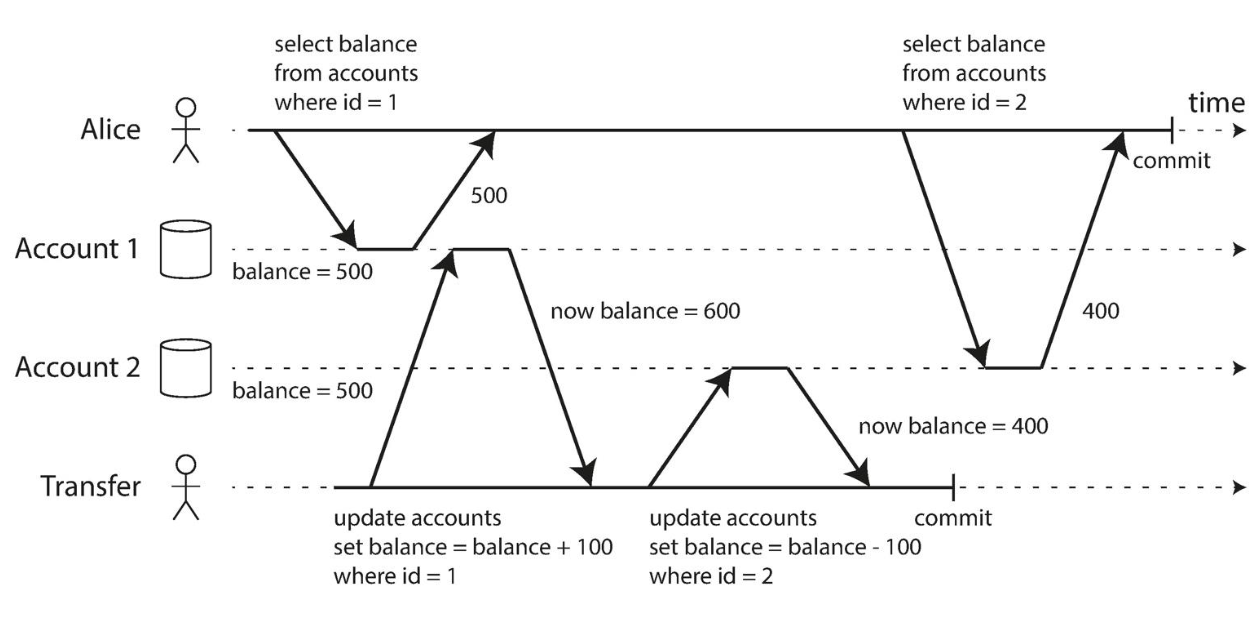
\includegraphics{images/12/readcommitted_issue.png}
   \caption{Read committed issue: Alice might think that her whole balance is 900, whilst it is 1000.}
   \label{fig:12/readcommitted_issue}
\end{figure}
% \begin{definition}
%    [Phantom Read]
%    A \textbf{phantom read} occurs when a transaction reads a set of records that satisfy a certain condition, but when it reads the same records again, the set of records has changed.

\subsection{Snapshot Isolation}
Snapshot isolation is a more relaxed isolation level than serializable isolation, but it is still stricter than Read Committed isolation.

In snapshot isolation, a transaction reads a snapshot of the database at the beginning of the transaction and writes to the database at the end of the transaction.

The snapshot allows transactions to see all the data that was commited at the start of the transaction.

% // TODO there is some other stuff about explicit locks, I'm not sure how important it is, the slides are a bit messed up

\note{It is possible to use at databases some techniques for locking the database, using locks or atomic operations. 
However it is costful}

\section{Write Skew and Phantoms}

\begin{paracol}{2}
   
   \begin{definition}
      [Write Skew]
      A \textbf{write skew} occurs when two transactions read the same data, then update ---possibly separate--- objects based on the read data, and then commit, causing a conflict.
   \end{definition}
   
   \switchcolumn

   \begin{figure}[htbp]
      \centering
      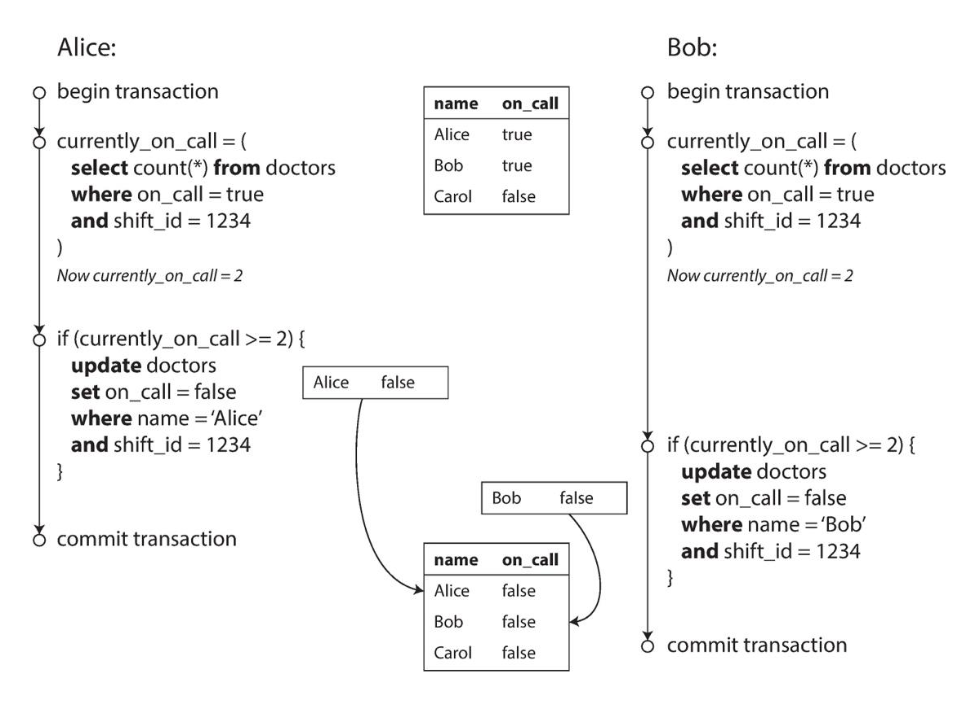
\includegraphics{images/12/write_skew.png}
      \caption{Both doctors read that \lstinline|currently_on_call >= 2| and ``leave the hospital'', causing no doctor to be on call \frownie.}
      \label{fig:12/write_skew}
   \end{figure}
\end{paracol}

There are some techniques to avoid write skew, such as using row locks or atomic operations, but we did not discuss them pretty much.



\chapter{Type Inference}
\begin{figure}[htbp]
   \centering
   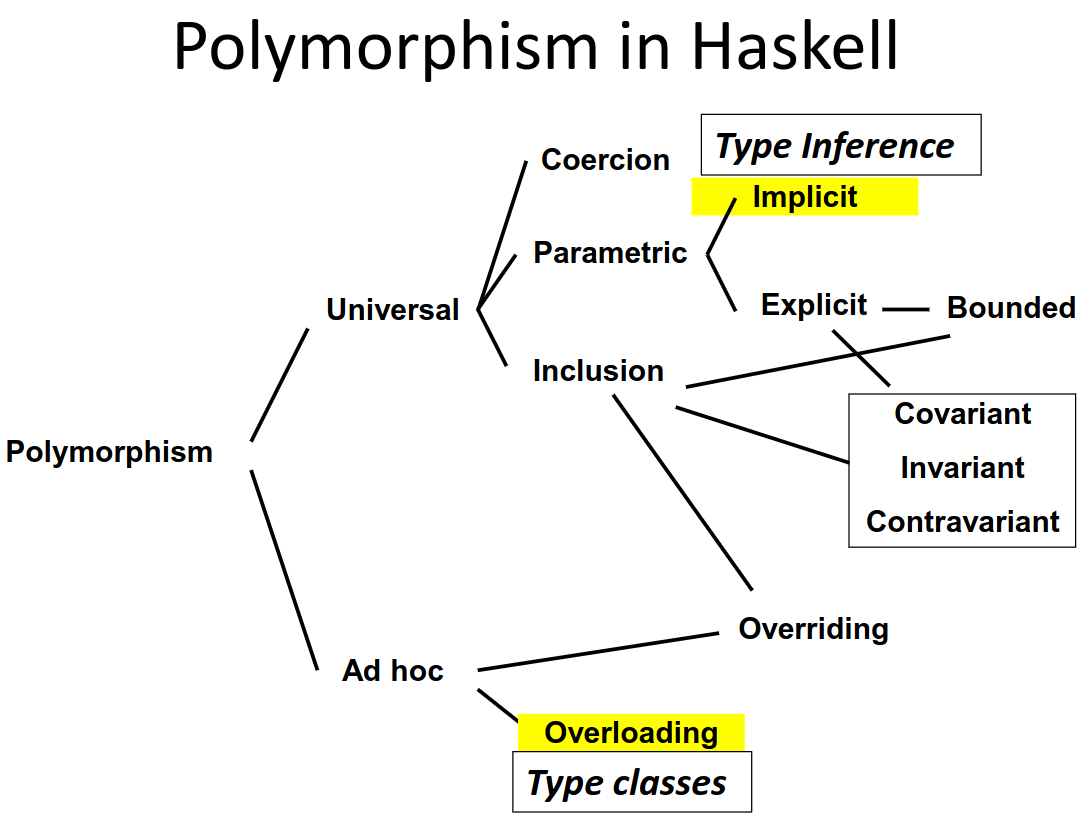
\includegraphics{images/haskell_polymorphism.png}
   \caption{Haskell Polymorphism Recap}
   \label{fig:haskell_polymorphism}
\end{figure}

\section{Overloading}
Haskell allows \textbf{overloading} even of \textbf{primitive types}:
the code to be executed is determined by the type of the arguments,
leading to have \textit{early binding} in \textit{statically} typed languages
or \textit{late binding} in \textit{dynamically} typed languages.

In Haskell we can write the following, but what is the type?
\begin{lstlisting}
   sqr x = x * x
\end{lstlisting}

When considering overloading besides arithmetic, we find that some functions are \textbf{fully polymorphic}:
\begin{lstlisting}
   length :: [w] -> Int
\end{lstlisting}

While others not so much;
for example, \textit{membership} works only for types that support equality,
while \textit{sorting} works only for types which support \textit{ordering}. 
\begin{lstlisting}
   member :: [w] -> w -> Bool
   sort :: [w] -> [w]
\end{lstlisting}

\section{Type Classes}
\textbf{Type Classes} solve many overloading problems concerning arithmetic and equality (and similar properties) support.

The idea is to generalize ML’s eqtypes to arbitrary types
and provide concise types to describe overloaded
functions, so no exponential blow-up (i.e. defining functions for every possible combination of type arguments).\\
Type classes allow users to define functions using overloaded
operations {---}e.g. square, squares, and member{---} and to
declare new collections of
overloaded functions: equality and arithmetic
operators are not privileged built-ins.
Haskell's solutions fits perfectly within type inference framework.

The intuition is that a sorting function may allow to be passed a comparison \lstinline|cmp| operator as argument,
thus making the function parametric.
\begin{lstlisting}
   qsort:: (a -> a -> Bool) -> [a] -> [a]
   qsort cmp [] = []
   qsort cmp (x:xs) = qsort cmp (filter (cmp x) xs) ++ [x] ++
   qsort cmp (filter (not.cmp x) xs)
\end{lstlisting}

Developing this idea, consider rewriting the parabola function to take operators as argument
\begin{lstlisting}
   parabola x = (x * x) + x
   parabola' (plus, times) x = plus (times x x) x
\end{lstlisting}
Here the extra parameter is a \textit{\textbf{dictionary}} that provides implementations for the overloaded ops.
These implies rewriting calls to pass appropriate implementations for plus and times:
\begin{lstlisting}
   y = parabola'(intPlus,intTimes) 10
   z = parabola'(floatPlus, floatTimes) 3.14
\end{lstlisting}

\begin{enumerate}
   \item Type class declarations
   \begin{enumerate}
      \item Define a set of operations, give it a name
      \item Example: \lstinline|Eq a| type class
      • operations \lstinline|==| and \lstinline|\=| with \lstinline|type a -> a -> Bool|
   \end{enumerate}
   \item Type class instance declarations
   \begin{enumerate}
      \item Specify the implementations for a particular type
      \item For \lstinline|Int| instance, \lstinline|==| is defined to be integer equality
   \end{enumerate}
   \item Qualified types (or Type Constraints)
   Concisely express the operations required on otherwise polymorphic type
   \lstinline|member:: Eq w => w -> [w] -> Bool|
\end{enumerate}

\labelitemize{
   \textit{implementation summary}
}{
   \begin{enumerate}
      \item Each overloaded symbol has to be introduced in at least one type class
      \item The compiler translates each function that uses an overloaded symbol into a function with an extra parameter: the dictionary.
      \item References to overloaded symbols are rewritten by the compiler to lookup the symbol in the dictionary.
      \item The compiler converts each type class declaration into a dictionary type declaration and a set of selector functions.
      \item The compiler converts each instance declaration into a dictionary of the appropriate type.
      \item The compiler rewrites calls to overloaded functions to pass a dictionary. It uses the static, qualified type of the function to select the dictionary.
   \end{enumerate}
}

\subsection{Compositionality}
\begin{lstlisting}
   class Eq a where
   (==) :: a -> a -> Bool
   instance Eq Int where
   (==) = intEq -- intEq primitive equality
   instance (Eq a, Eq b) => Eq(a,b) where
   (u,v) == (x,y) = (u == x) && (v == y)
   instance Eq a => Eq [a] where
   (==) [] [] = True
   (==) (x:xs) (y:ys) = x==y && xs == ys
   (==) _ _ = False
\end{lstlisting}

\subsection{Compound Translation}
\newpage
\subsection{Subclasses}
\begin{paracol}{2}
   \vspace{\fill}
   
   A subclass declaration expresses this relationship:
   \begin{lstlisting}
      class Eq a => Num a where
      (+) :: a -> a -> a
      (*) :: a -> a -> a
   \end{lstlisting}
• With that declaration, we can simplify the type of the function

\begin{lstlisting}
   memsq :: (Eq a, Num a) => a -> [a] -> Bool
   memsq x xs = member (square x) xs
\end{lstlisting}

\vspace{\fill}
\switchcolumn

\begin{figure}[htbp]
   \centering
   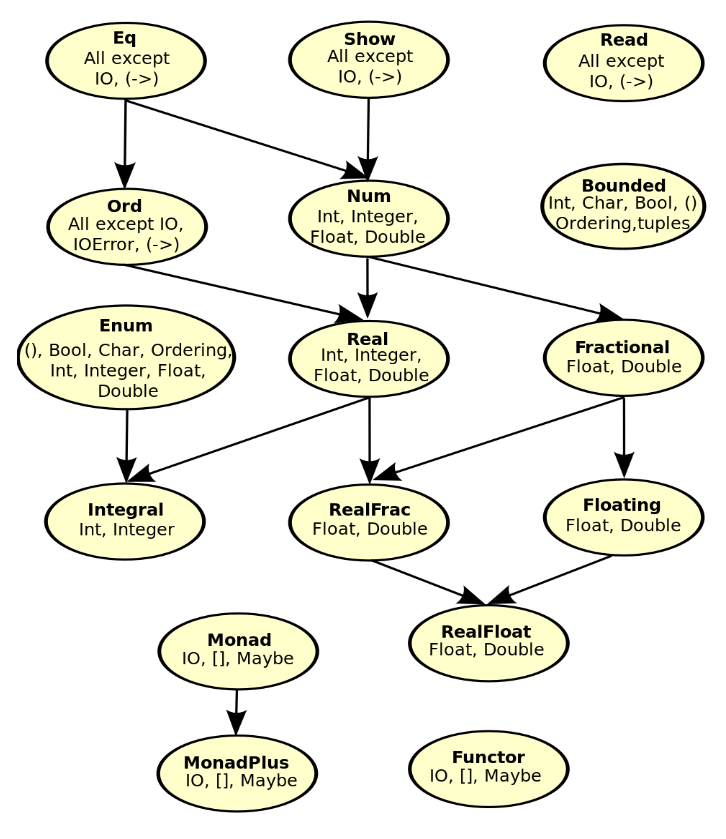
\includegraphics{images/haskell_subclasses.png}
   \caption{Haskell Subclasses relationships}
   \label{fig:haskell_subclasses}
\end{figure}

\end{paracol}

\subsection{Deriving}
For Read, Show, Bounded, Enum, Eq, and Ord, the compiler
can generate instance declarations automatically.
\begin{lstlisting}
   data Color = Red | Green | Blue
      deriving (Show, Read, Eq, Ord)
   
   Main>:t show
   show :: Show a => a -> String
   Main> show Red
   "Red"
   Main> Red < Green
   True
   Main>:t read
   read :: Read a => String -> a
   Main> let c :: Color = read "Red"
   Main> c
   Red
\end{lstlisting}

\subsection{Numeric Literals}
\begin{lstlisting}
   class Num a where
      (+) :: a -> a -> a
      (-) :: a -> a -> a
      fromInteger :: Integer -> a
      -- Even literals are overloaded.
      -- 1 :: (Num a) => a
      ...

   inc :: Num a => a -> a
   inc x = x + 1
\end{lstlisting}

\labelitemize{
   \textit{Advantages}
}{
   \setlength{\leftskip}{1em}
   Numeric literals can be interpreted as values of any
   appropriate numeric type,
   for example: 1 can be an Integer or a Float or a user-
   defined numeric type.
}

\subsection{Missing Notes}
Look at slides $34...64$ for more on Type Inference.

\section{Inferencing types}
In standard type checking the compiler examine body of each function and uses declared types to check agreement;
type inference instead consists in examining code without type information, and infer the
most general types that could have been declared

\subsection{Steps schematics}
\begin{figure}[htbp]
   \centering
   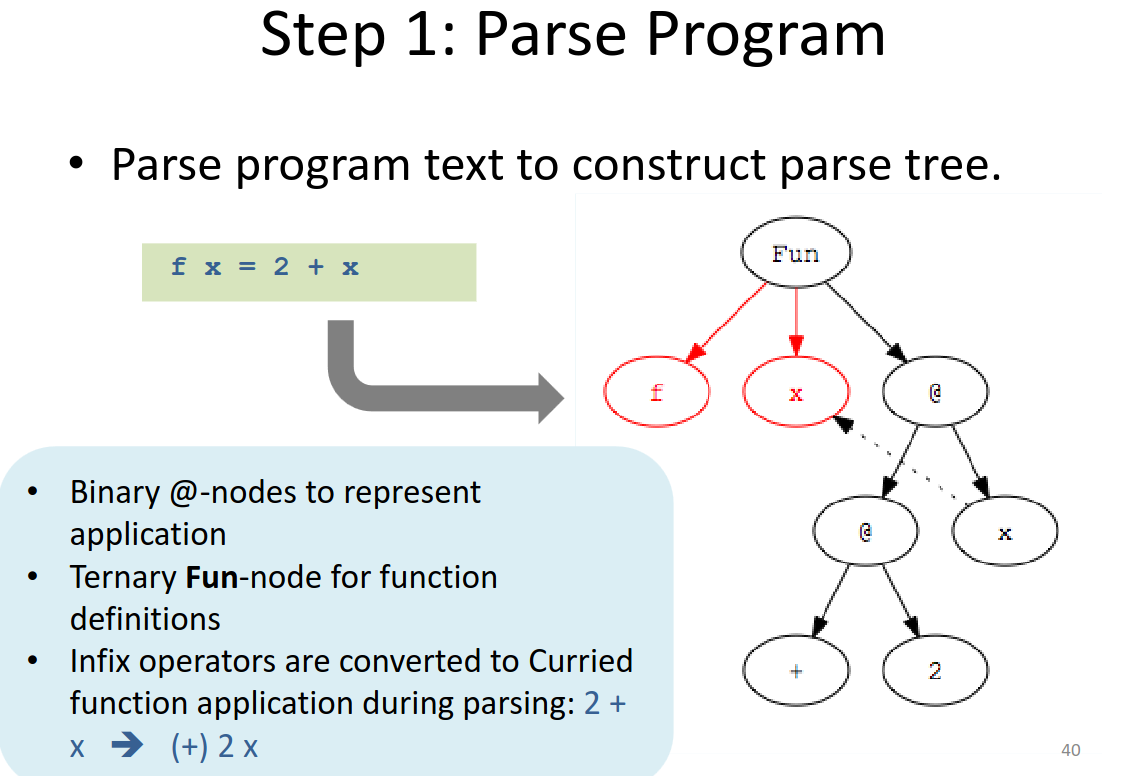
\includegraphics[width=0.4\columnwidth]{images/typeinference_step1.png}
   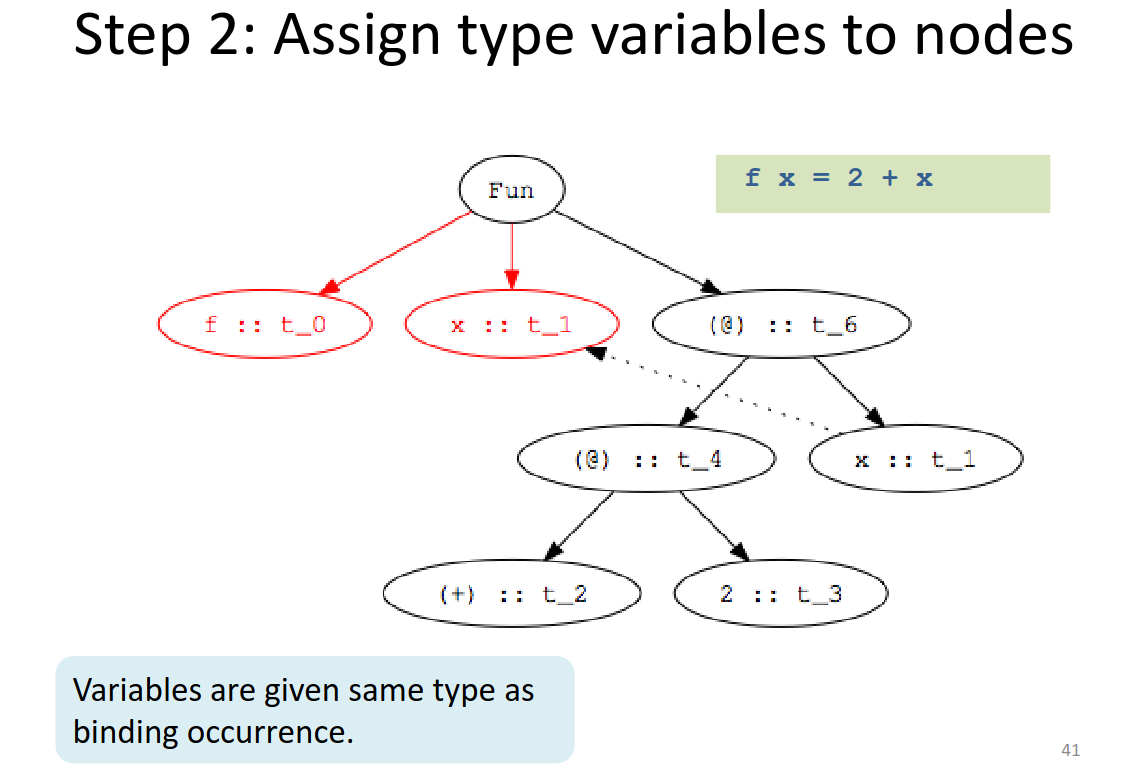
\includegraphics[width=0.4\columnwidth]{images/typeinference_step2.png}
   \label{fig:typeinference_step1_2}
\end{figure}

% \begin{figure}[htbp]
%    \centering
%    \label{fig:typeinference_step2}
% \end{figure}

\textbf{Constraints} can be deduced from (function) \textit{Application} nodes \lstinline|f x| and from \textit{Abstractions} \lstinline|f x = e|.

\begin{figure}[htbp]
   \centering
   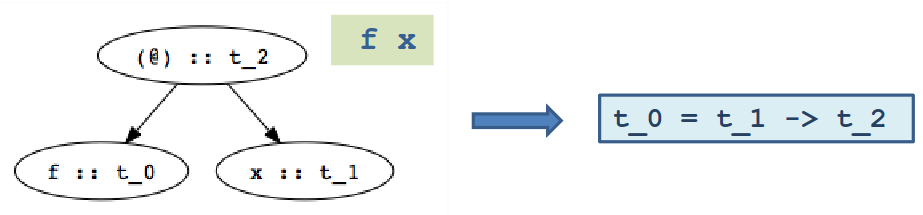
\includegraphics{images/typeinference_constraints_application.png}
   \caption{Deducing constraints from function application}
   \label{fig:typeinference_constraints_application}
\end{figure}
\begin{itemize}
   \item Type of \lstinline|f| (\lstinline|t_0| in figure) must be $domain \longrightarrow range$.
   \item \textbf{Domain} of \lstinline|f| must be type of argument \lstinline|x| (\lstinline|t_1|)
   \item \textbf{Range} of f must be result of application (\lstinline|t_2|)
   \item \textbf{Constraint}: \lstinline|t_0 = t_1 -> t_2|
\end{itemize}

\begin{figure}[htbp]
   \centering
   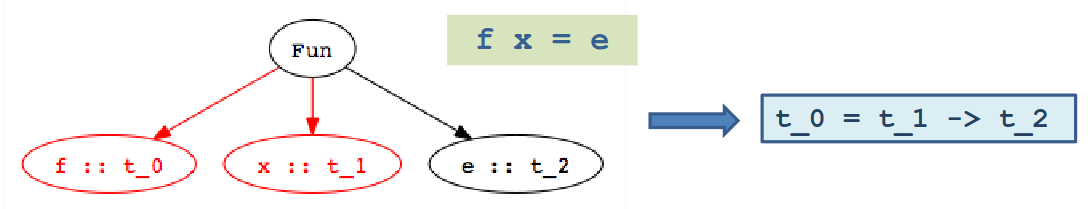
\includegraphics{images/typeinference_constraints_abstraction.png}
   \caption{Deducing constraints from abstractions}
   \label{fig:typeinference_constraints_abstraction}
\end{figure}

\begin{itemize}
   \item Type of \lstinline|f| (\lstinline|t_0|) must $domain \longrightarrow range$
   \item \textbf{Domain} is type of abstracted variable \lstinline|x| (\lstinline|t_1|)
   \item \textbf{Range} is type of function body \lstinline|e| (\lstinline|t_2|)
   \item \textbf{Constraint}: \lstinline|t_0 = t_1 -> t_2|
\end{itemize}

\begin{figure}[htbp]
   \centering
   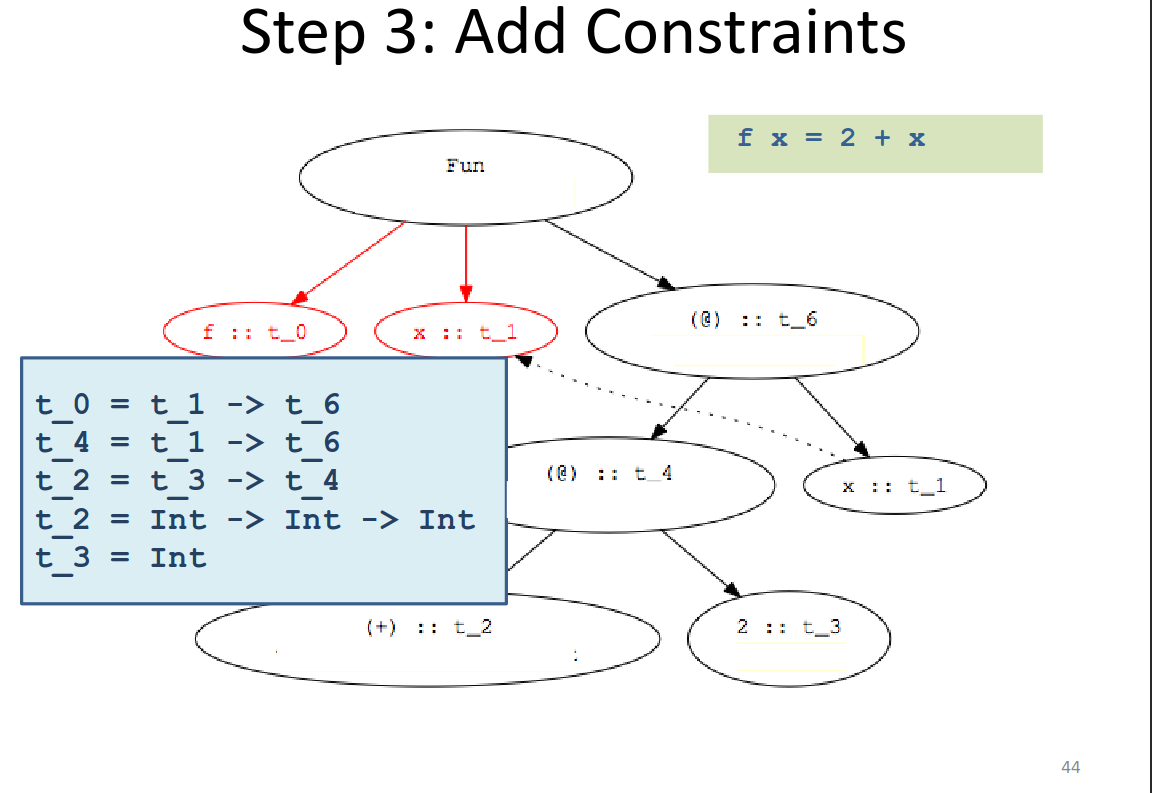
\includegraphics[width=0.4\columnwidth]{images/typeinference_step3.png}
   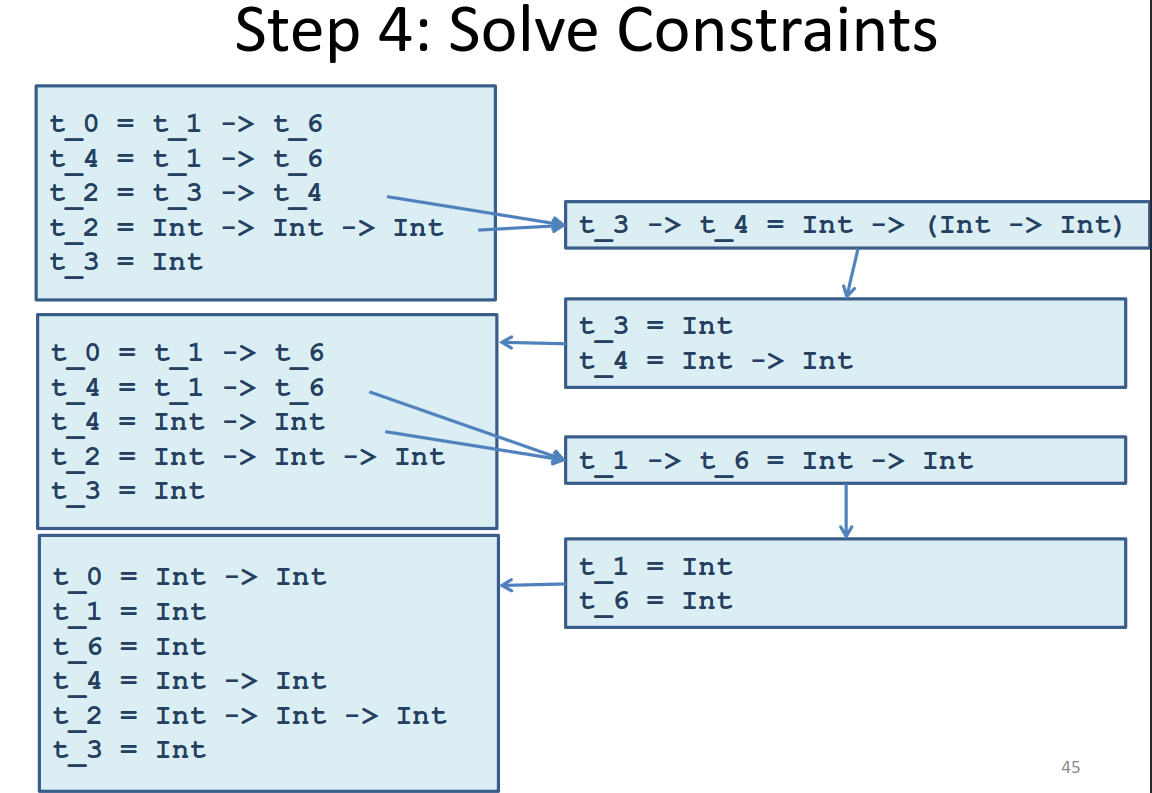
\includegraphics[width=0.4\columnwidth]{images/typeinference_step4.png}
   \label{fig:typeinference_step3_4}
\end{figure}

\begin{figure}[htbp]
   \centering
   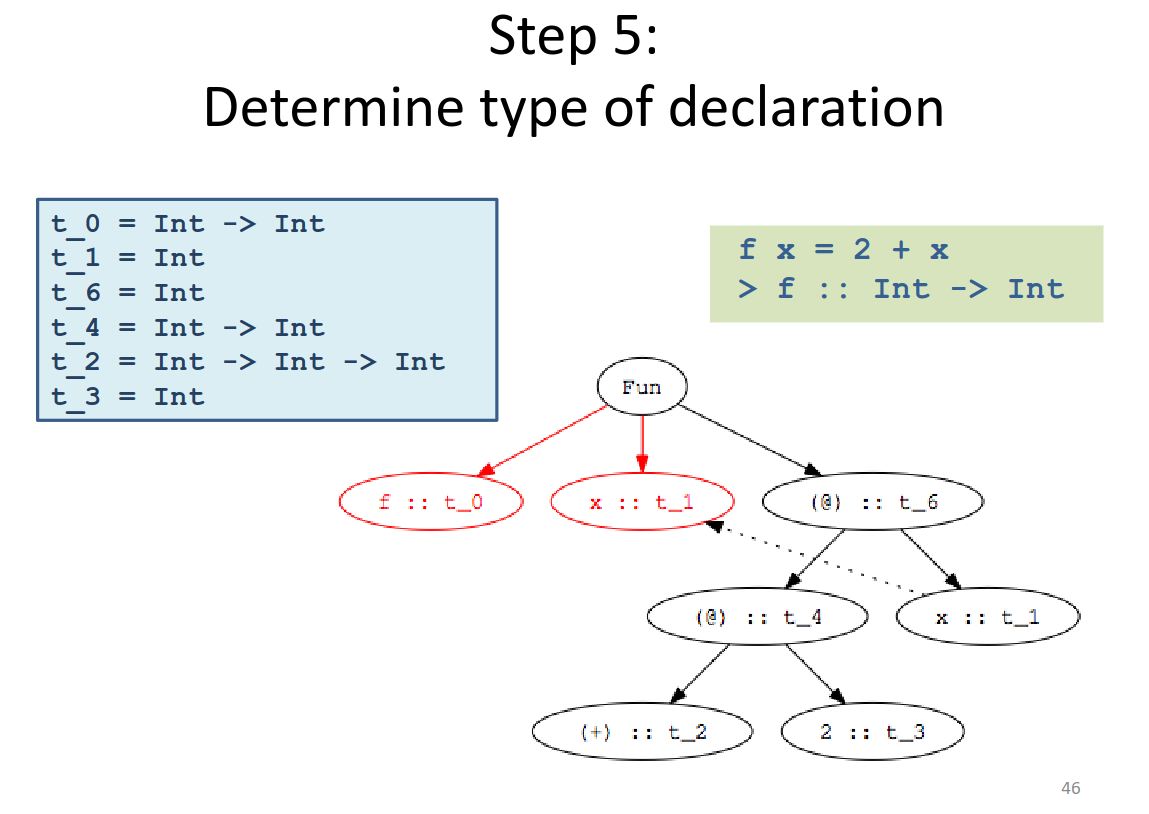
\includegraphics[width=0.4\columnwidth]{images/typeinference_step5.png}
   \label{fig:typeinference_step5}
\end{figure}

\subsubsection{Steps summary}
\begin{enumerate}
   \item Parse program to build parse tree
   \item Assign type variables to nodes in tree
   \item Generate constraints:
   \begin{enumerate}
      \item From environment: constants (\lstinline|2|), built-in
      operators (\lstinline|+|), known functions (\lstinline|tail|).
      \item From shape of parse tree: e.g., application and
      abstraction nodes.
   \end{enumerate}
   \item Solve constraints using unification
   \item Determine types of top-level declarations
\end{enumerate}

\subsection{Polymorphism}

In general \textbf{unconstrained} type variables become \textbf{polymorphic types};
for instance, in the example below \lstinline|t_4| is unconstrained, hence we get a polymorphic type:
\begin{lstlisting}
   f g = g 2
   > f :: (Int -> t_4) -> t_4
\end{lstlisting}
\nl

For functions with multiple clauses, i.e. \textit{polymorphic datatypes},
for each clause a separate type is inferred, 
and then the resulting types are combined by adding constraints such as that all clauses have the same type.
In case of \textit{recursive calls}:
the function has same type as its definition.

\begin{lstlisting}
   append ([],r) = r
   append (x:xs, r) = x : append (xs, r)
\end{lstlisting}

\begin{enumerate}
   \item Infer type of each clause
   \begin{enumerate}
      \item First clause:
      \begin{lstlisting}
   > append :: ([t_1], t_2) -> t_2
      \end{lstlisting}
      \item Second clause:
      \begin{lstlisting}
   > append :: ([t_3], t_4) -> [t_3]
      \end{lstlisting}
   \end{enumerate}
   \item Combine by equating types of two clauses
   \begin{lstlisting}
   > append :: ([t_1], [t_1]) -> [t_1]
   \end{lstlisting}
\end{enumerate}

\subsection{Overloading}
In presence of \textbf{overloading} (\textit{Type Classes}), type inference infers a \textbf{qualified type} \lstinline|Q => T|
\begin{itemize}
   \item T is a Hindley Milner type, inferred as seen before
   \item Q is set of type class predicates, called a constraint
\end{itemize}
\begin{lstlisting}
   example :: Ord a => a -> [a] -> Bool
   example z xs = 
      case xs of
         [] -> False
         (y:ys) -> y > z || (y==z && ys == [z])
\end{lstlisting}

\begin{paracol}{2}
   \colfill
   In the example \textbf{Type} \lstinline|T| is \lstinline|a -> [a] -> Bool|
   while the \textbf{Constraint} \lstinline|Q| is \lstinline|{ Ord a, Eq a, Eq [a]}|.
   \lstinline|Q| later simplifies\footnote{According to some rules not discussed here} to \lstinline|Ord a|
   \colfill
   \switchcolumn

   \begin{itemize}
      \item \lstinline|Ord  a| because \lstinline|y>z|
      \item \lstinline|Eq a| because \lstinline|y==z|
      \item \lstinline|Eq [a]| because \lstinline|ys == [z]|
   \end{itemize}
\end{paracol}
\subsubsection{Functor and \texttt{fmap}}
\chapter{Solidity Attacks}
Solidity is a high-level language whose syntax is similar to that of JavaScript. It is designed to target the Ethereum Virtual Machine (EVM). Solidity is statically typed, supports inheritance, libraries and complex user-defined types among other features. It is used to implement smart contracts on various blockchain platforms, the most popular of which is Ethereum.

\section{DAO attack}
The DAO (Decentralized Autonomous Organization) was a smart contract that was created to act as a venture capital fund for the Ethereum ecosystem. It was launched in April 2016 and raised over \$150 million in Ether, making it the largest crowdfunding campaign in history at the time. The DAO was designed to allow investors to vote on which projects to fund and to receive a share of the profits from those projects.

The DAO was implemented as a smart contract on the Ethereum blockchain using Solidity. The contract was designed to allow investors to deposit Ether into the contract in exchange for DAO tokens, which could be used to vote on proposals for funding. The contract also contained a function that allowed investors to withdraw their Ether at any time.

In June 2016, an attacker exploited a vulnerability in the DAO contract that allowed them to drain funds from the contract. The attacker used a recursive call attack to repeatedly call the withdraw function on the contract, draining over \$50 million in Ether before the attack was stopped.

\subsection{Reentrancy attack}
The \textbf{reentrancy attack} is a type of attack that exploits a vulnerability in a smart contract that allows an attacker to \ul{repeatedly call a function on the contract before the previous call has completed}. This can allow the attacker to drain funds from the contract or perform other malicious actions.

The DAO attack was a reentrancy attack that exploited a vulnerability in the DAO contract that allowed the attacker to repeatedly call the withdraw function on the contract before the previous call had completed. This allowed the attacker to drain funds from the contract by repeatedly withdrawing Ether from the contract.

To prevent it from happening, the contract should be designed in such a way that it is not possible for an external contract to call the withdraw function before the previous call has completed. This can be done by using the \texttt{require} statement to check that the contract is in a valid state before allowing the function to proceed, or using \texttt{send()} or \texttt{transfer()} instead of \texttt{call.value()}.

\section{Arithmetic overflow and underflow}
Arithmetic overflow and underflow are common vulnerabilities in smart contracts that can lead to unexpected behavior and security issues. An overflow occurs when the result of an arithmetic operation exceeds the maximum value that can be stored in the data type used to represent the result. An underflow occurs when the result of an arithmetic operation is less than the minimum value that can be stored in the data type used to represent the result.

A good prevention strategy is to use the SafeMath library, which provides functions for performing arithmetic operations that check for overflows and underflows and revert the transaction if an overflow or underflow is detected.
\ul{Never use Solidity arithmetic operators directly, always use SafeMath functions.}

\section{Phishing}
Phishing is a type of attack where an attacker tries to trick a user into revealing sensitive information, such as passwords or private keys, by impersonating a legitimate entity. Phishing attacks are common in the cryptocurrency space, where attackers try to steal funds by tricking users into revealing their private keys or other sensitive information.
\chapter{Lambdas in KJava}
The purpose of lambdas was enabling ---without requiring recompilation of existing binaries--- functional programming in Java, that is being able to pass behaviors as well as data to functions, and to introduce lazy evaluation with stream processing.
\section{Java 8}
\lstset{style=javaBlock}
\begin{lstlisting}
   List<Integer> intSeq = Arrays.asList(1,2,3);
   intSeq.forEach(x -> System.out.println(x));
   // equivalent syntax
   intSeq.forEach((Integer x) -> System.out.println(x));
   intSeq.forEach(x -> {System.out.println(x);});
   intSeq.forEach(System.out::println); //method reference
\end{lstlisting}

Note that class variables used inside the body of a lambda must be \lstinline|final| or \textit{effectively} \lstinline|final|, or have to be static.
This is \ul{fundamental design choice, as it makes \textbf{closures}\footnote{A closure is a function that captures the lexical context in which it was defined.} not necessary}.
\begin{lstlisting}
   int var = 10; // must be [effectively] final
   intSeq.forEach(x -> System.out.println(x + var));
   // var = 3; // uncommenting this line it does not compile
\end{lstlisting}
\begin{lstlisting}
public class SVCExample { // static variable capture
   private static int var = 10;
   public static void main(String[] args) {
      List<Integer> intSeq = Arrays.asList(1,2,3);
      static int var = 10;
   
      intSeq.forEach(x -> System.out.println(x + var));
      var = 3; // OK! it compiles
}}
   \end{lstlisting}

\section{Functional Interfaces}
\subsection{Implementation}
The Java 8 compiler conceptually first converts a lambda
expression into a function, compiling its code; 
then it generates code to call the compiled function where
needed.\\
For example, \lstinline|x -> System.out.println(x)| could be
converted into a generated static function
\begin{lstlisting}
   public static void genName(Integer x) {
      System.out.println(x);
   }
\end{lstlisting}


\ul{But what \textbf{type} should be generated for this function? How
should it be called? What class should it go in?}

\subsection{Functional Interfaces}

Java 8 \textit{lambdas} are instances of \textit{functional interfaces},
which are java interfaces with exactly \textit{one} \textit{\textbf{abstract}} method.

\begin{lstlisting}
   public interface Comparator<T> { //java.util
      int compare(T o1, T o2);
   }
   public interface Runnable { //java.lang
      void run();
   }
   public interface Consumer<T>{ //java.util.function
      void accept(T t)
   }
   public interface Callable<V> {//java.util.concurrent
      V call() throws Exception;
   }
\end{lstlisting}
{Functional Interfaces can be used as target type of lambda
expressions, i.e.\ns
\begin{itemize}
	\item As type of variable to which the lambda is assigned
	\item As type of formal parameter to which the lambda is passed
\end{itemize}}

The lambda is invoked by calling the only abstract method
of the functional interface;
lambdas can be interpreted as instances of anonymous
inner classes implementing the functional interface.

For instance, recalling the \lstinline|forEach| presented earlier, the corresponding interface is the following.
Note that it must be checked that the lambda matches the \lstinline|forEach| signature defined in the interface:
\begin{lstlisting}
intSeq.forEach(x -> System.out.println(x));

// List<T> extends Iterable<T>
interface Iterable<T>{ //java.lang
   default void forEach(Consumer<? super T> action)
      for (T t : this)
         action.accept(t);
\end{lstlisting}

Lambdas could, in principle, be compiled as instances of anonymous inner classes, but there is no default strategy for compiling lambdas indicated in neither JLS8 nor JVMS8. The compiler can choose to compile them as anonymous inner classes, or it can choose to use \lstinline|invokedynamic| to implement them, as it is usually done nowdays.

\subsubsection{Default Methods}
Adding new abstract methods to interfaces breaks existing implementations of such interface.
To avoid this, Java 8 introduced \textit{default methods} in interfaces, which are methods with a body that can be overridden by implementing classes,
enforcing backward compatibility with existing solutions.

\subsubsection{Method References}
\textbf{Method references} can be used to pass an existing
function in places where a lambda is expected,
but their signature needs to
match the signature of the functional interface method required.
\begin{table}[htbp]
   \centering
   \begin{tabular}{|c|c|c|}
      \hline
      static  & \lstinline|ClassName::StaticMethodName| & \lstinline|String::valueOf|\\
      constructor &  \lstinline|ClassName::new| & \lstinline|ArrayList::new|\\
      specific object instance & \lstinline|objectReference::MethodName| & \lstinline|x::toString|\\
      arbitrary object of a given type & \lstinline|ClassName::InstanceMethodName| & \lstinline|Object::toString|\\
      \hline
   \end{tabular}
   \caption{Method references examples}
   \label{tab:method_references}
\end{table}
\chapter{Distributed Messaging}
Messaging systems enable loose coupling and asynchronous communication between distributed components, they act as the glue binding components together.

When applied to distributed computing, messaging systems can be used to implement a wide range of communication patterns, such as request/reply, publish/subscribe, and event sourcing.
A too simplified message passing mechanism may not be enough, since it must take into account delays, message ordering, lost packets, scalability, and fault tolerance.

\section{Message Passing mechanisms}

\begin{itemize}
   \item Request-response - a client sends a request to a server, and the server sends a response back.
   \item One-way messaging - a client sends a message to a server, and the server does not send a response.
   \item Publish-subscribe - a client subscribes to a topic, and the server sends messages to all clients subscribed to that topic.
\end{itemize}


Publish-subscribe is useful because allows to receive information from multiple services, explicitly (and implicitly) categorize them, and assign them different semantics.

\subsection{Adapting Publish-subscribe to Point-to-point}
Note however that trying to create point-to-point communication with publish-subscribe may be cumbersome, and lead to un-elegant architectures, like having all clients subscribing to everyone else: a mess.

Introducing a server in the middle simplifies the topology, and allows to have a single point of contact for all clients, which forwards messages to the correct recipient.
On the other hand, it is not distributed, not scalable, and may become a bottleneck!

We could also have single queues for each client, but this is not scalable, and may lead to a single point of failure, again.

\section{Message Brokers - Kafka}
Message brokers are software systems that receive messages from producers and deliver them to consumers. They act as intermediaries between producers and consumers, and can provide additional features such as message storage, routing, and filtering.

Kafka is a distributed message broker that is designed for high-throughput, fault-tolerant, and scalable messaging. It is used in a wide range of use cases, such as log aggregation, stream processing, and event sourcing.

Messages in Kafka are similar to DB rows, and are stored in topics, which are similar to DB tables. Each message has a key, a value, and a timestamp, and is stored in a partition.

Messages are written in \textit{Batches}, which are collections of messages produced to the same topic and partition within a short time window. Batching improves throughput and reduces latency, but is a tradeoff: larger batches allows for more messages to be stored, but it might take longer for a message to be propagated.
\\


Messages are categorized into \textbf{topics}, which in turn are broken down into \textbf{partitions}, where they are written in append-only fashion and are read in order from beginning to end.
Each partition can be hosted on a different server, hence a single topic may be scaled horizontally across multiple servers to \textbf{scale-out}.


\ul{Multiple partitions imply there's not guarantee of message time-ordering across the entire topic.}

Kafka sacrifices a global order of messages for scalability, and allows to have multiple consumers reading from the same topic, and even the same partition\footnote{if they belong to different groups. This will be discussed later} at the same time.
In general it is not impossible to have a global order ---see blockchains--- but it may be very costful in a distributed environment.\\
However, \ul{if it is necessary for a topic to have a global order, it is possible to have a single partition for that topic.}

\framedt{Bypassing the Single partition limitation}{
   To avoid having a single partition but still preserve the order, we can implement some trick.

   Suppose you have a topic for ``user tracking'', with each user being identified by a key.\\
   You could create a partition for odd user IDs and one for even user IDs, and then have a single consumer for each partition.
}

\subsection{Producers and Consumers}

Producers write messages to topics, and consumers read messages from topics. Producers and consumers can be scaled horizontally to improve throughput and fault tolerance.
Scaling out consumers allows to consume message-intense topics. 

The \textbf{offset} is a unique identifier for each message within a partition, and is used by consumers to keep track of their progress. The offset is always increased, and is never reset.

Note that, in order to preserve the ordering of the message within a partition, \ul{a partition may be consumed only by one member of a consumer group at a time}.\\
In this way, the sequential semantics of a partition are preserved.\\
This implies that the maximum degree of scalability is given by the number of partitions, and not by the number of consumers.

\subsubsection{Rebalancing}
The number of partitions is set when the topic is created, and in general cannot be changed during the provisioning of the topic.\\
However, Kafka has a feature called \textit{rebalancing}, which allows to dynamically create partitions, allowing for more consumers to consume from the same topic.
However, it is a bit of a mess, and requires the provisioning to stop, compute the rebalancing plan, and then restart the provisioning.

\subsubsection{Brokers and Clusters}
A single Kafka server is called a \textit{broker}, and a group of brokers is called a \textit{cluster}. Each broker is responsible for a set of partitions, and is able to handle reads and writes for those partitions.

Brokers communicate with each other to \textbf{replicate} data and keep the cluster in sync. Each partition has a leader broker, which is responsible for handling reads and writes for that partition in the cluster. The leader broker replicates data to follower brokers, which can take over as leader if the current leader fails.

Consumers always get messages from the leader, never from the replicas, allowing to enforce asynchronous consistency.

\subsubsection{Retention}

For each topic it is possible to define a retention policy, which specifies how long messages should be retained in the topic. Messages can be retained for a fixed amount of time, or until a certain size limit is reached.

Kafka brokers are configured with a default retention
setting for topics, defining either size or time limits, which once reached, messages are deleted.


\subsubsection{Multiple Groups}

\begin{figure}[htbp]
   \centering
   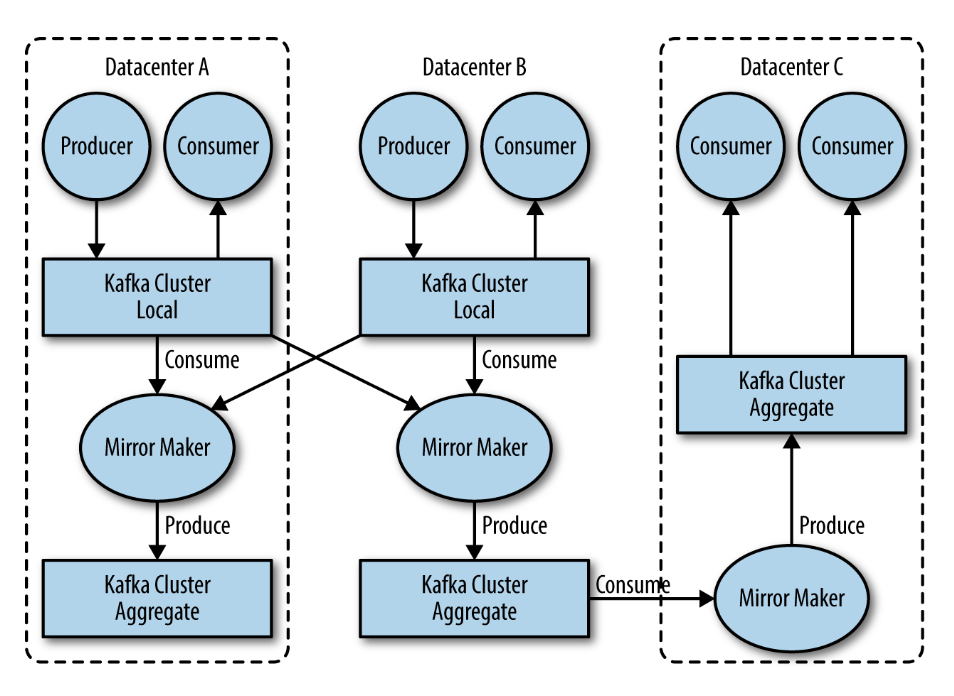
\includegraphics{images/16/clusters.png}
   \caption{Clusters and \texttt{MirrorMaker}s schema}
   \label{fig:16/clusters}
\end{figure}

As kafka deployments grow, it is often advantageous to have multiple clusters, in order to have \textbf{segregation}, \textbf{isolation}, and \textbf{fault tolerance}.

When working with multiple datacenters
it could be required that messages be
copied between them.
Kafka includes a tool called \texttt{MirrorMaker},
used for this purpose, which simply is a Kafka consumer and producer, linked together with a queue:
messages are consumed from one Kafka cluster and produced for another

\section{Using Kafka}


\subsection{Producers}
First addressing the producer point of view, it is important to consider the requirements on this side:
\begin{itemize}
   \item Is every message critical?
   \item Are accidental duplicates acceptable?
   \item Are there latency or throughput requirements?
\end{itemize}
These questions are important to correctly use the API for the producer, which can be either \texttt{fire-and-forget}, \texttt{synchronous}, or \texttt{asynchronous}.

\begin{itemize}
   \item \texttt{fire-and-forget} - the producer sends the message and does not wait for a response. Kafka automatically retries to send messages if they fail to be delivered, so most of them will be actually delivered, but some may be lost.
   \item \texttt{synchronous} - the producer sends the message and waits for a response. This is the safest way to send messages, but it is also the slowest.
   \lstinline|send()| returns a \lstinline|Future()| object, which we may invoke \lstinline|get()| on to wait for the response.
   \item \texttt{asynchronous} - the producer invokes \lstinline|send()| along with a \textit{callback} and continues with its execution.
   The callback is invoked when the message is successfully delivered, or when an error occurs.
\end{itemize}

\newpage
\subsubsection{Message record format}
\begin{paracol}{2}
   \begin{itemize}
      \item Topic
      \item Key  (optional)
      \item Partition  (optional)
      \item Value
   \end{itemize}
   
   Once sent the \texttt{ProducerRecord}, the
   producer will serialize the key and value
   objects so can be sent over the network.\\
   Later on, if a partition is
   specified in the \texttt{ProducerRecord}, the partitioner simply returns the partition we specified.
   
   A separate thread is responsible for sending those batches of records to the appropriate Kafka brokers,
   which yield a Metadata record upon successful delivery.


   \switchcolumn

   \begin{figure}[htbp]
      \centering
      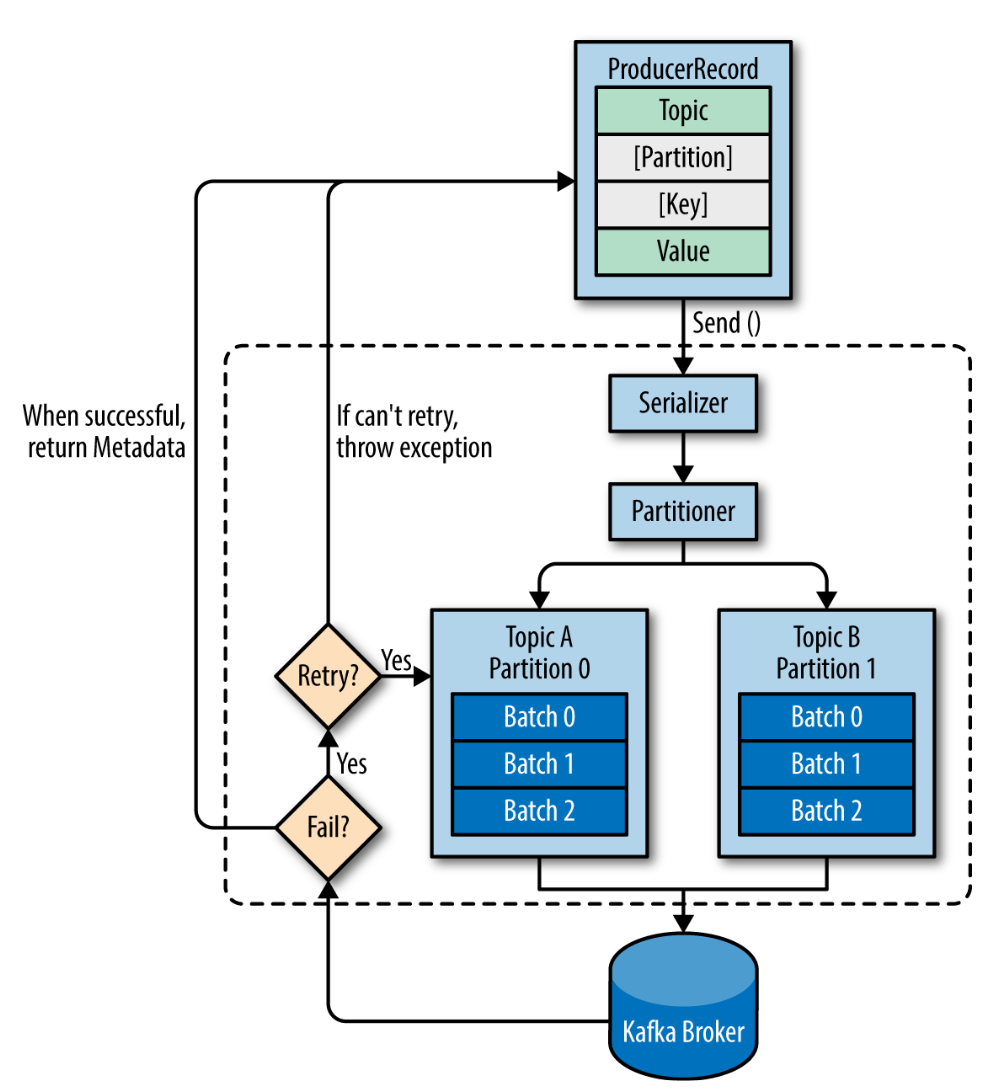
\includegraphics{images/16/producerRecord.png}
      \caption{Sending \texttt{ProducerRecord}}
      \label{fig:16/producerRecord}
   \end{figure}

\end{paracol}


\subsection{Consumers}

When dealing with Kafka messages it is important to consider that the producers may write to topics at a rate higher than the consumers can read from them.\\
This is undesirable, as it may lead to the consumers falling behind, and eventually running out of memory;
hence, we must allow to scale the consumers.

Kafka consumers are typically part of a group. When multiple consumers are subscribed to a topic and belong to the same group, each consumer in the group will receive messages from a different subset of the partitions in the topic.

\begin{figure}[htbp]
	\centering
	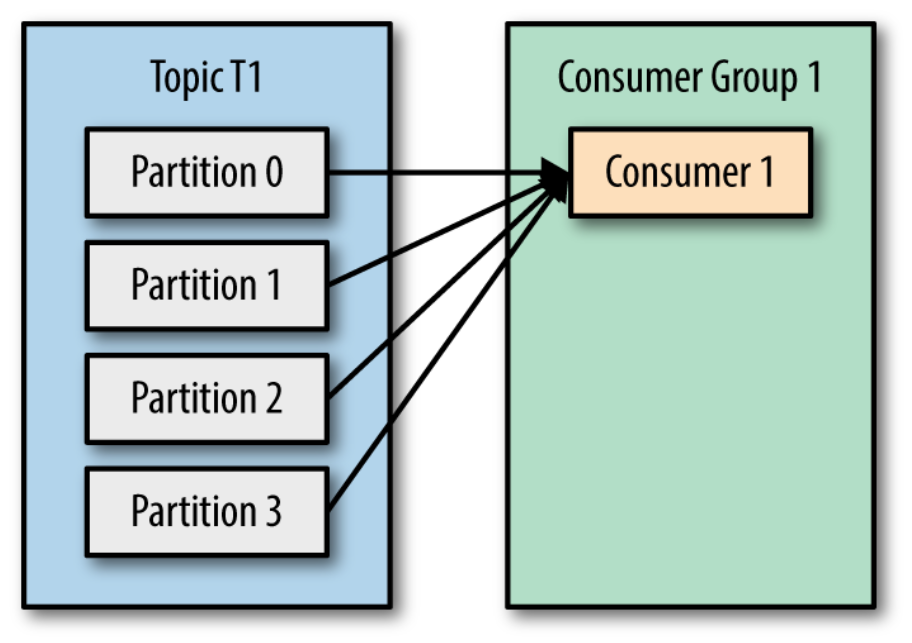
\includegraphics[width=0.3\columnwidth]{images/16/partitions_1.png}
	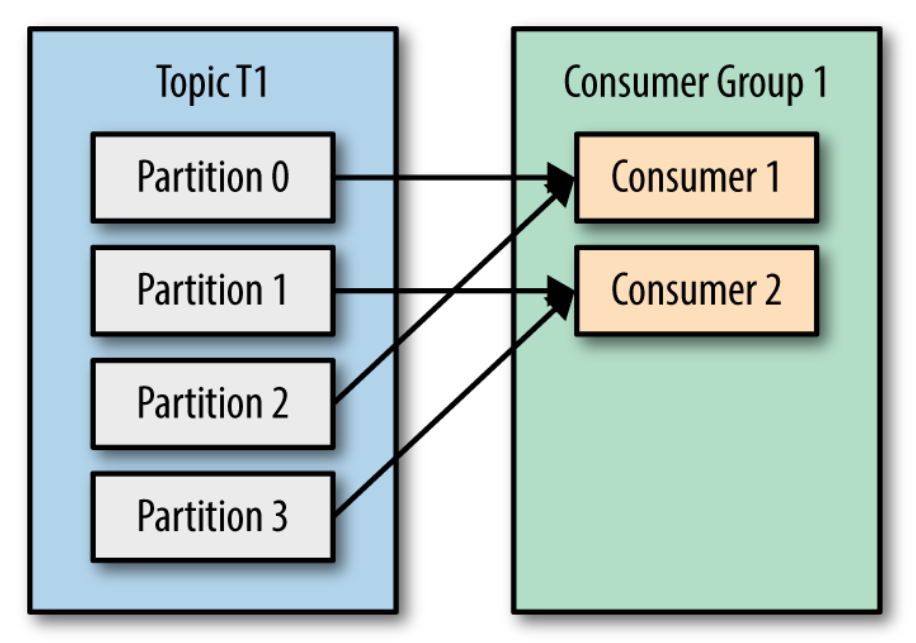
\includegraphics[width=0.3\columnwidth]{images/16/partitions_2.png}
	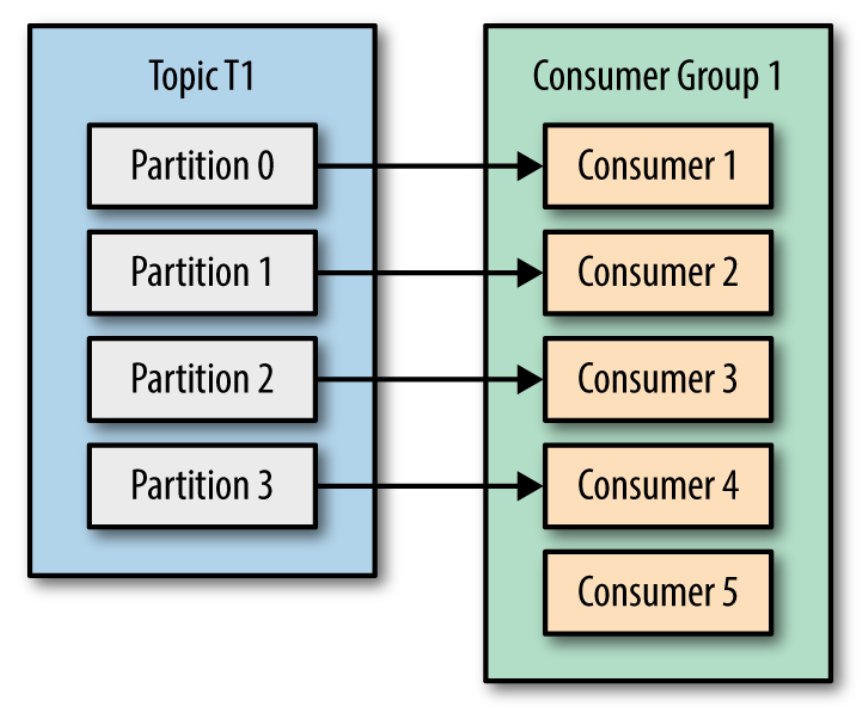
\includegraphics[width=0.3\columnwidth]{images/16/partitions_3.png}
	\caption{Partitions are assigned to Consumers to have a fair distribution.}
	\label{fig:16/partitions_1}
\end{figure}

Having more consumers than partitions is not a problem, as the consumers will simply be idle.\\
In general it is reasonable to have many partitions, allowing to scale when needed.

\begin{paracol}{2}
   It is not uncommon to have multiple applications that need to receive the same data.
   Simply assigning different consumers groups to different applications ensures that messages are delivered to all of them.
   \note{The separation among consumers remains.}
   \switchcolumn
   \begin{figure}[htbp]
      \centering
      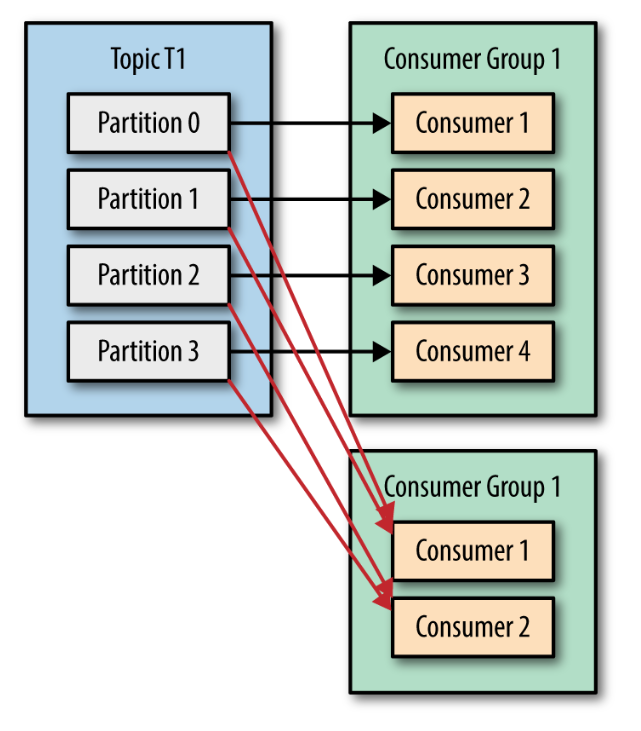
\includegraphics[width=0.5\columnwidth]{images/16/groups.png}
      \caption{Multiple Consumer Groups}
      \label{fig:16/groups}
   \end{figure}
\end{paracol}


\subsection{Rebalancing}

Moving partition ownership from one consumer to another is called a \textbf{rebalance}. Rebalances are important because they provide the consumer group with high availability and scalability,
but \ul{in the normal course of events they are \textit{fairly undesirable}}, because during a rebalance, \ul{consumers can’t consume messages}, so a rebalance is basically a short \textbf{window of unavailability} of the entire consumer group.

When partitions are moved from one consumer to another, the consumer loses its current state; if it was caching any data, it will need to refresh its caches—slowing down the application until the consumer sets up its state again.

\subsubsection{When is it needed?}
\begin{itemize}
   \item A new consumer joins the group
   \item A consumer leaves the group
   \item A consumer is considered dead
   \item The set of partitions for a topic changes
\end{itemize}

The most interesting case is when a consumer ``dies''.
If the consumer stops sending heartbeats for long enough, its session will time
out and, after a few seconds, the group coordinator will consider it ``dead'' and \ul{trigger a rebalance}.
During those seconds, no messages will be processed from the partitions owned by the dead consumer \frownie.

Instead, when closing a consumer cleanly, the consumer will notify the group coordinator that it is leaving, and the group coordinator will trigger a rebalance immediately.

\section{Kafka Strengths}
Kafka is able to seamlessly handle multiple producers, whether those clients
are using many topics or the same topic, and multiple consumers, whether they are in the same group or different groups, and also allow to seamlessly read from the same stream without interfering with each other, opposed to many queuing systems where once a message is consumed by one client, it is not available to any other.

Disk-based retention allows consumers to avoid working necessarily in real-time, and to catch up with the stream at their own pace.
\chapter{Frameworks and IOC}
\section{Frameworks}

A \textbf{Software Framework}
is a collection of common code
providing generic functionality that can be selectively
overridden or specialized by user code providing
specific functionality.\\
An \textbf{Application Framework} is a software framework used to
implement the standard structure of an \textit{application} for
a specific development environment.

\labelitemize{Examples}{

   \begin{enumerate}
      \item General Software Frameworks
      \begin{enumerate}
         \item \texttt{.NET}
         \item \texttt{Android SDK}
         \item \texttt{Cocoa}
         \item \texttt{Eclipse}
      \end{enumerate}
      \item GUI Frameworks
      \begin{enumerate}
         \item \texttt{MFC}
         \item \texttt{Gnome}
         \item \texttt{Qt}
      \end{enumerate}
      \item Web Frameworks
      \begin{enumerate}
         \item \texttt{ASP.NET}
         \item \texttt{Rails}
         \item \texttt{GWT}
         \item \texttt{Spring}
         \item \texttt{Flask}
      \end{enumerate}
   \end{enumerate}
}

A framework embodies some \textit{abstract design}, with
more behavior built in.
In order to use it you need to insert your behavior into various places in the framework either by subclassing or by plugging in your own classes,
then 
the framework’s code, which handles the program's \textbf{control flow} (the ``\texttt{main} execution''), then calls your code at these points.\\
This realizes a very general concept, emphasizing \textbf{inversion of
control} as opposed to libraries,
where the user's code calls the library one,
here is the code of the framework that calls the user's one.

\subsection{Component Frameworks}
\textbf{Componenent Frameworks} support development, deployment, composition
and execution of components designed according to a given
\textbf{Component Model}.
More specifically, they support \textbf{composition/connection} of components according to
the mechanisms provided by the \textit{Component Model},
allowing instances to be "plugged" into the
component framework itself,
and regulating their \textbf{interaction}.

\subsubsection{IDE and Frameworks}
\textbf{NetBeans} is both an \texttt{IDE} and supports the \texttt{JavaBeans} \textit{Component Framework}.\\
In general a framework can be supported by several \texttt{IDE}s
\note{
   e.g. \texttt{Spring} supported by \texttt{Spring Tool Suite} (based
   on \texttt{Eclipse}), \texttt{NetBeans}, \texttt{IntelliJ IDEA}, \texttt{Eclipse}, ...
} 
While an \texttt{IDE} can support several frameworks
\note{
   e.g \texttt{NetBeans} supports \texttt{JavaBeans}, \texttt{Spring}, \texttt{J2EE},
   \texttt{Maven}, \texttt{Hibernate}, \texttt{JavaServer Faces}, \texttt{Struts}, \texttt{Qt}, ...
} 

\subsection{Features}
Consists of \textbf{parts} that are found in many apps of that type
\begin{itemize}
   \item \textbf{Libraries} with APIs (classes with methods etc.)
   \item Ready-made extensible programs (``\textbf{engines}'')
   \item Sometimes also \textbf{tools} (e.g. for development, configuration,
   content)
\end{itemize}
They also provide reusable abstractions of code wrapped in a well-defined API,
however recall that,unlike in libraries,
the overall program's \textbf{flow of control} is \textit{not} dictated by the caller, but by the \textit{framework}.
\nl

Frameworks usually support extensibility,
either by extending within the framework language {---} using, subclassing, overriding, implementing interfaces, registering event handlers, ...{---} or through plug-ins defined in a specific format.
 

\section{Inversion of Control}
\subsection{GUI}
In \textit{text-based interaction}, the order of interactions
and of invocations is decided by the the code,
while in the \textit{\textbf{GUI}-based interaction}, the \textit{GUI} loop decides
when to invoke the methods (listeners), based on the
order of events.

\begin{figure}[htbp]
   \centering
   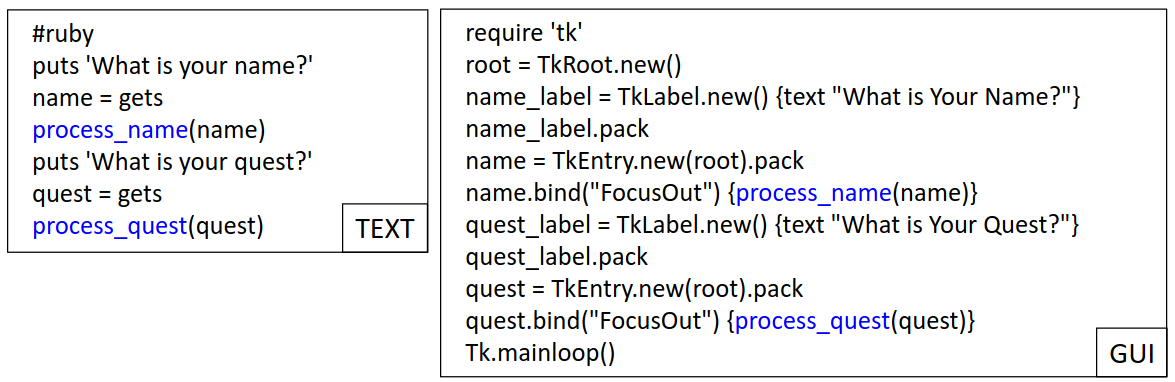
\includegraphics{images/ioc_textgui.png}
   \caption{Text vs GUI interaction}
   \label{fig:ioc_textgui}
\end{figure}

\begin{figure}[htbp]
   \centering
   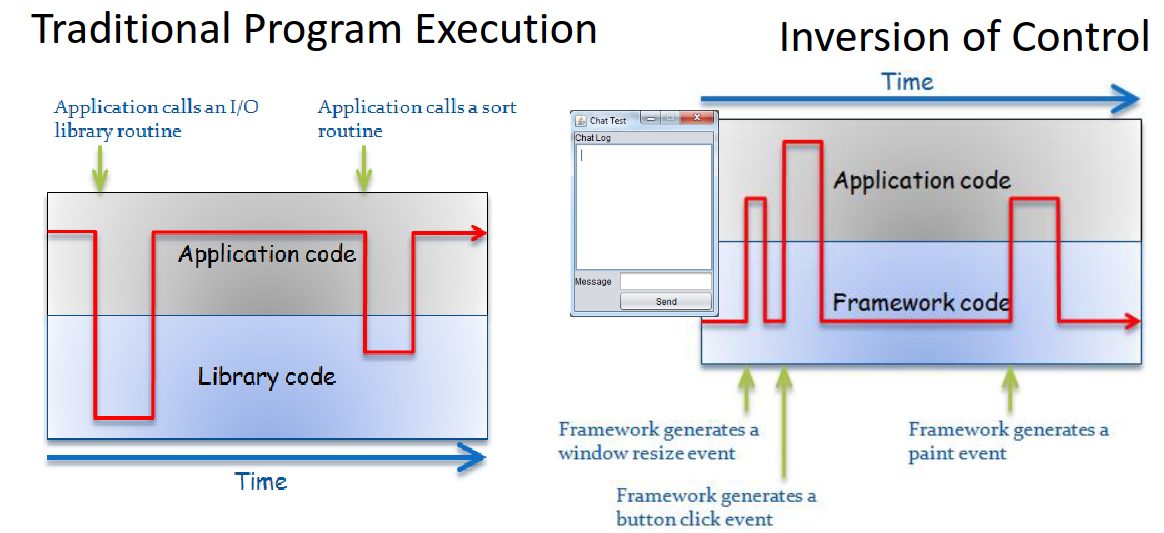
\includegraphics{images/ioc_fwvslib.png}
   \caption{IoC: Library vs Framework approach}
   \label{fig:ioc_fwvslib}
\end{figure}

\subsection{Containers}
Often Frameworks provide \textbf{containers} for deploying
\textit{components}:
a container may provide at \textit{runtime functionalities}
needed by the components to execute.

For examples \texttt{EJB} containers are responsible of the
persistent storage of data and of the availability of
\texttt{EJB}’s for all authorized clients.

\section{Dependency Injection}
Good \textit{OO Systems} should be organised as
a network of interacting objects,
keeping in mind as a goal to have \textit{high \textbf{cohesion}}, \textit{low \textbf{coupling}}.\\
{Low coupling has as key advantages\ns
\begin{itemize}
   \item Extensibility
   \item Testability
   \item Reusability
\end{itemize}}

When discussing \textbf{IoC} in Frameworks, \textit{``Control''} does not refer only to control flow, but also \ul{control over \textit{dependencies}, \textit{coupling}, \textit{configuration}}.
A component gives up control to a framework and agrees to play by some rules.

\ul{\textbf{Dependency Injection} (DI) is a design pattern for achieving Inversion of Control} (IoC), where the responsibility of creating and managing dependencies is moved from the objects themselves to an external system (often the framework).


In traditional programming, objects often create their dependencies manually using the \lstinline|new| keyword. This can lead to tightly coupled code, making testing, maintenance, and scaling more difficult. Dependency Injection reverses this by delegating the responsibility of dependency creation to an external mechanism.\\
So, a class (consumer) requires certain objects (dependencies) to function properly, and instead of instantiating these objects directly, we have to are ``inject'' them into the class from the outside.

In the following section we discuss an example of a \textit{TradeMonitor} class, and how to refactor it to use \textit{Dependency Injection}.

\subsection{Trade Monitor}
Let's discuss this example to see how all of this comes into practice.
\begin{center}
   \textit{A trader wants that the system rejects trades when the exposure reaches a certain limit}
\end{center}

Thus the component (class) \texttt{TradeMonitor} provides
a method \texttt{TryTrade} (below) which checks the condition,
accessing \textit{current exposure} and \textit{exposure limit} from a \texttt{DAO} (\textit{Data Access Object}), a persistent storage.
\begin{lstlisting}
   public bool TryTrade(string symbol, int amount){
      int limit = limitDao.GetLimit(symbol);
      int exposure = limitDao.GetExposure(symbol);
      return (exposure + amount > limit) ? false : true;
   }
\end{lstlisting}
How can we limit dependencies among the two components?
\subsection{Interfaces - Refactoring 1}
Let's consider a possible refactoring, introducing \textbf{interface} and implementation separation,
which still has a static dependency on \texttt{DAO} :
\begin{figure}[htbp]
   \centering
   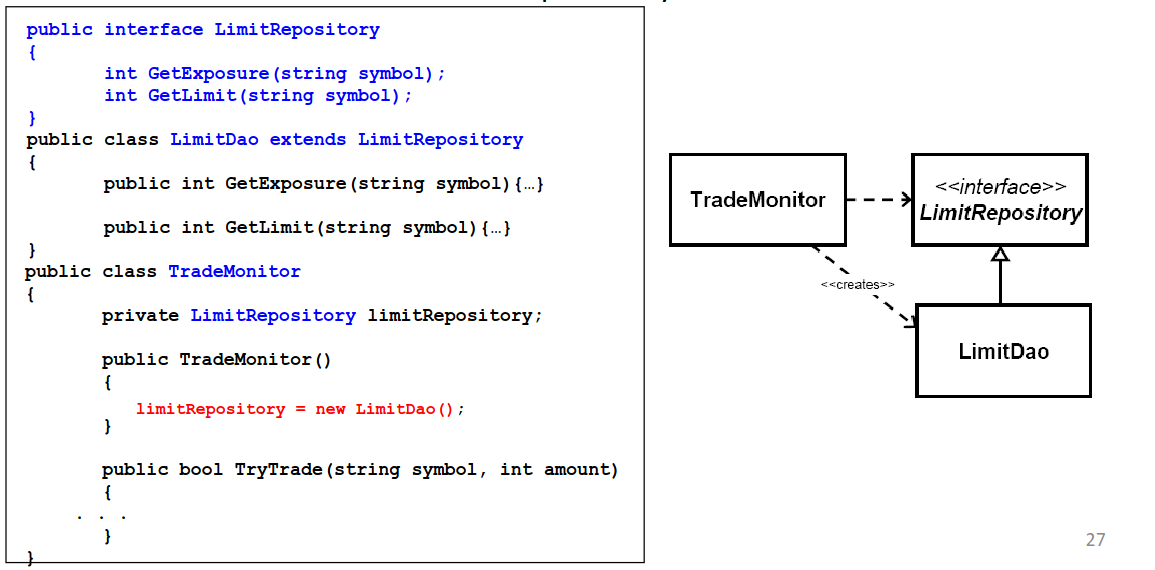
\includegraphics{images/trademonitor_ref1.png}
   \caption{Refactoring 1}
   \label{fig:trademonitor_ref1}
\end{figure}

\subsection{Factory - Refactoring 2}
Here we introduce a \textbf{factory} which resolves the previous problem, but \texttt{LimitDao} is still tightly coupled, but to \texttt{Factory}.

\begin{figure}[htbp]
   \centering
   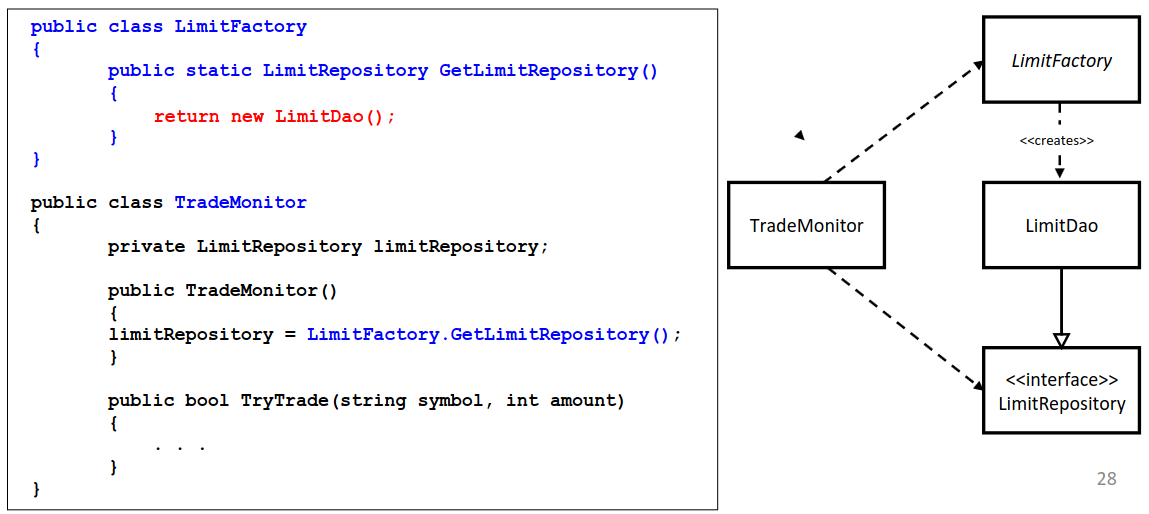
\includegraphics{images/trademonitor_ref2.png}
   \caption{Refactoring 2}
   \label{fig:trademonitor_ref2}
\end{figure}

\subsection{ServiceLocator - Refactoring 3}
Introduce a \texttt{ServiceLocator}. This object acts as a (static)
registry for the \texttt{LimitDao} you need,
giving us extensibility, testability, reusability.\\
However ote that an external \texttt{Assembler} sets up the registry.

\begin{figure}[htbp]
   \centering
   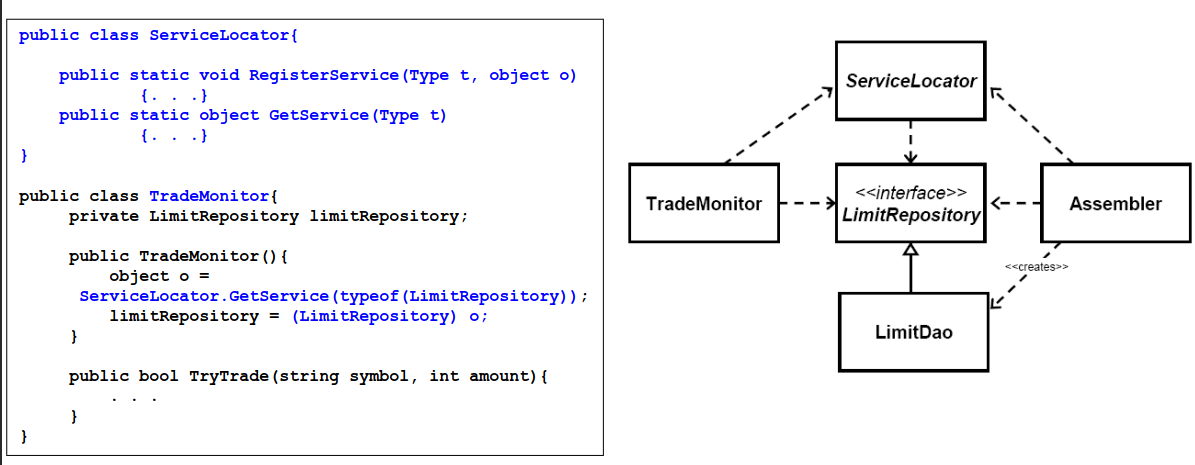
\includegraphics[width=0.7\columnwidth]{images/trademonitor_ref3.png}
   \caption{Refactoring 3}
   \label{fig:trademonitor_ref3}
\end{figure}

\labelitemize{
   \color{darkgreen}
   \textit{Pros}
}{
   \color{darkgreen}
   \begin{itemize}
      \item The Service Locator pattern succeeds in decoupling the TradeMonitor
      from the LimitDao
      \item Allows new components to be dynamically created and used by other
      components later
      \item It can be generalized in several ways, eg. to cover dynamic lookup
   \end{itemize}
}

\labelitemize{
   \color{darkred}
   \textit{Cons}
}{
   \color{darkred}
   \begin{itemize}
      \item Every component that needs a dependency must have a reference to the
      service locator
      \item All components need to be registered with the service locator
      \item If bound by name:
      \begin{itemize}
         \item Services can’t be type-checked
         \item Component has a dependency to the dependent component names
         \item if many components share an instance but later you want to specify different
      \end{itemize}
      instance for some, this becomes difficult
      \item If bound by type can only bind one instance of a type in a container
      \item Code needs to handle lookup problems
   \end{itemize}
}

\subsection{Different techniques}

\begin{figure}[htbp]
   \centering
   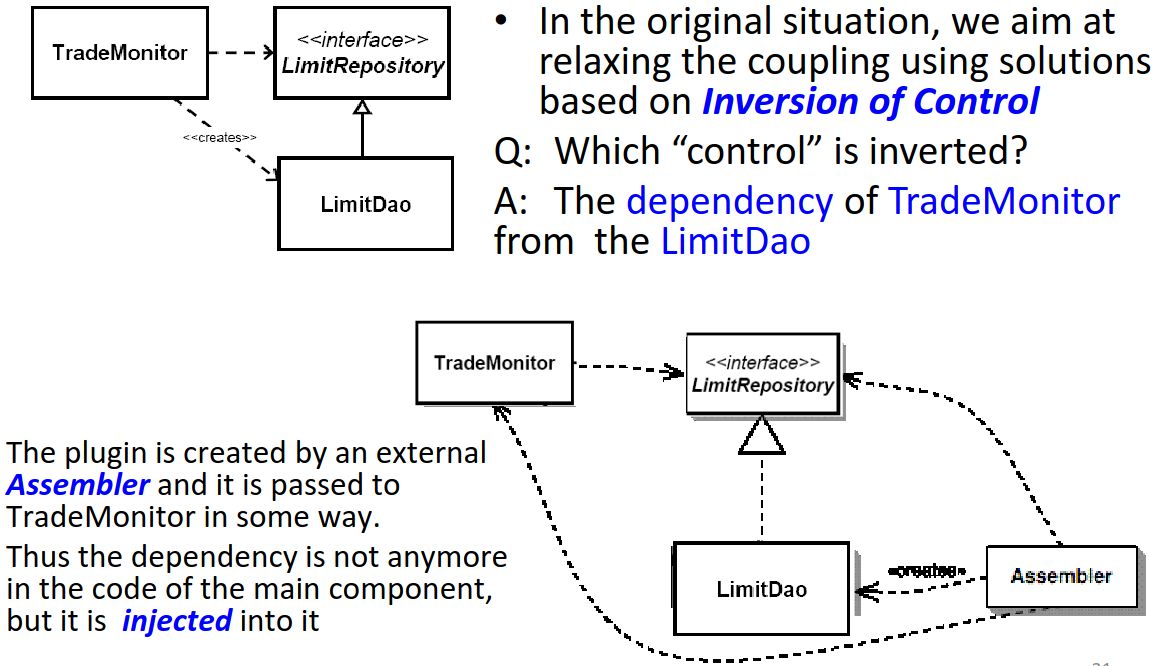
\includegraphics{images/dependency_inj.png}
   % \caption{}
   \label{fig:dependency_inj}
\end{figure}

\textbf{Dependency injection} allows avoiding \textit{hard-coded}
dependencies (strong coupling) and changing them, and allows selection among multiple implementations of a given dependency interface at run time.
It can be achieved through:
\begin{enumerate}
   \item Setter injection
   \item Constructor injection
   \item (Interface injection)
\end{enumerate}

Both \textbf{Service Locator} and \textbf{Dependency Injection} provide
the desired decoupling, but let's compare the two solutions: 
\begin{itemize}
   \item 
   With service locator there is no \textbf{IoC}, since the desired component is obtained
   after request by the \texttt{TradeMonitor} to the \texttt{Locator};
   this makes the application still depending on the locator.
   \item With dependency injection there is \textit{no explicit request}: the
   component appears in the application class.
\end{itemize}
Inversion of control is a bit harder to understand.
With Service Locator the application still depends on the
locator, besides, it is easier to find dependencies of component if \textit{Dependency Injection} is used.
% // TODO better understand service locator vs dependency injection
\begin{center}
   \color{darkgray}
   Check \textit{constructors} and \textit{setters}\\vs\\Check \textit{all invocations} to
   \texttt{Locator} in the source code
\end{center}

\section{Designing Frameworks}
Frameworks are normally implemented in an object-oriented language such as Java.
It is important to learn to analyze a potential software family, identifying
its possible common and variable aspects, and evaluating
alternative framework architectures.
\nl

A possible idea is to start from a known divide-and-conquer algorithm such as the one in Lst. \ref{lst:divideandconquer_example} and try to generalize it to a framework.
\begin{lstlisting}[label={lst:divideandconquer_example},caption={Example pseudocode of a Divide-and-Conquer algorithm}]
   function solve (Problem p) returns Solution { 
      if isSimple(p)
         return simplySolve(p);
      else
         sp[] = decompose(p);
         for (i= 0; i < sp.length; i = i+1)
            sol[i] = solve(sp[i]);
         return combine(sol);
   }
\end{lstlisting}
We can apply known techniques and patterns to \textbf{define} a
\textit{framework} for a \textbf{software family}.
Instances of the defined framework, obtained by standard
extension mechanism, 
will be concrete algorithms of the \textit{family}.

\subsection{Terminology}
\begin{itemize}
   \item \textbf{Frozen Spot}\\
   common (shared) aspect of the software family, unmodifiable defined by the framework
   \item \textbf{Hot Spot}\\
   variable aspect of the family, defined by the user.
   A hot spot is represented by a group of abstract \textit{\textbf{hook} methods}.
   \item \textbf{Template method}\\
   concrete method of base (abstract) class implementing behavior common to all members of the family, such as the \texttt{solve} method in the example
   A template method calls a \textit{hook method} to invoke a function that is specific to one family member ---Inversion of Control---.
   \item \textbf{Hook method}\\
   abstract method of the base class, to be implemented by subclasses, such as \texttt{isSimple}, \texttt{simplySolve}, \texttt{decompose}, \texttt{combine} in the example
   \item A hot spot is realized in a framework as hot spot subsystem:
   \begin{figure}[htbp]
      \centering
      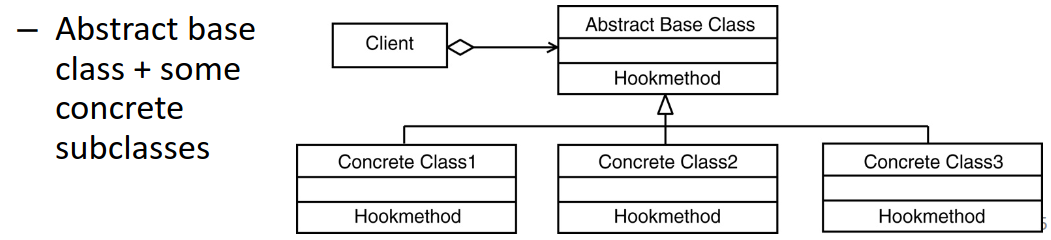
\includegraphics{images/hotspot.png}
      \caption{\textit{Hotspot} implementation}
      \label{fig:hotspot}
   \end{figure}
\end{itemize}
\labelitemize{
   \textit{Principles}
}{
   \begin{enumerate}
      \item The \textbf{unification} principle [\textit{Template Method} Design Pattern]
      \begin{enumerate}
         \item Exploits \textit{inheritance} to implement the hot spot subsystem
         \item Both the \ul{template methods and hook methods are defined in the same abstract base class}
         \item \ul{Hook methods are implemented in subclasses of the base class}
         
      \end{enumerate}
      \item The \textbf{separation} principle [\textit{Strategy} Design Pattern]
      \begin{enumerate}
         \item It uses \textit{delegation} to implement the hot spot subsystem
         \item The \ul{template methods are implemented in a \textbf{concrete} context class}; the \ul{hook methods are defined in a separate \texttt{abstract class} and implemented in its subclasses}
         \item The template methods delegate work to an instance of the
         subclass that implements the hook methods
      \end{enumerate}
   \end{enumerate}
}

\subsection{Template Method design pattern}
It is one of the behavioural pattern of the \textit{Gang of Four};
Its intent is to define the skeleton of an algorithm in an operation,
\textit{deferring} some steps to subclasses:
A \textbf{template method} belongs to an \textit{abstract} class and it defines an algorithm in terms of \textit{abstract} operations that subclasses \textbf{override}
to provide \textit{concrete behavior}.

{Template methods call, among others, the following operations:\ns
\begin{enumerate}
   \item \textbf{concrete} operations of the abstract class $\longrightarrow$ fixed parts of the algorithm
   \item \textbf{primitive} operations, $\longrightarrow$ abstract operations that subclasses have to implement
   \item \textbf{hook} operations $\longrightarrow$ provide default behavior that subclasses may override if necessary.\\
   A hook operation often does nothing by default.
\end{enumerate}}

\begin{figure}[htbp]
   \centering
   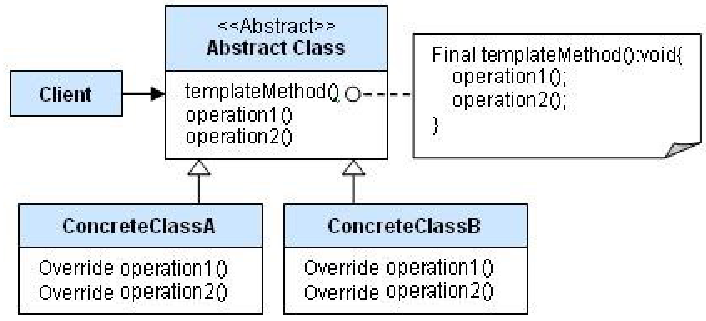
\includegraphics{images/dp_templatemethod.png}
   \caption{Template method}
   \label{fig:dp_templatemethod}
\end{figure}

\subsubsection{Applying \textit{Unification Principle}}
Let's consider the result of applying \textit{unification principle} to the example code \ref{lst:divideandconquer_example} provided before.
\lstset{
   morekeywords=[3]{solve,templatemethod},
   keywordstyle=[3]\color{green},
   morekeywords=[4]{hotspots,isSimple,simplySolve,decompose,combine},
   keywordstyle=[4]\color{red}
}
\begin{lstlisting}
   -- hotspots
   -- templatemethod
   abstract public class DivConqTemplate
   function solve (Problem p) returns Solution {
      if isSimple(p)
         return simplySolve(p);
      else
         sp[] = decompose(p);
         for (i= 0; i < sp.length; i = i+1)
            sol[i] = solve(sp[i]);
         return combine(sol);
   }
   abstract protected boolean isSimple (Problem p);
   abstract protected Solution simplySolve (Problem p);
   abstract protected Problem[] decompose (Problem p);
   abstract protected Solution combine(Problem p, Solution[] ss) ;
\end{lstlisting}
\lstset{style=javaBlockAnn}

\begin{figure}[htbp]
   \centering
   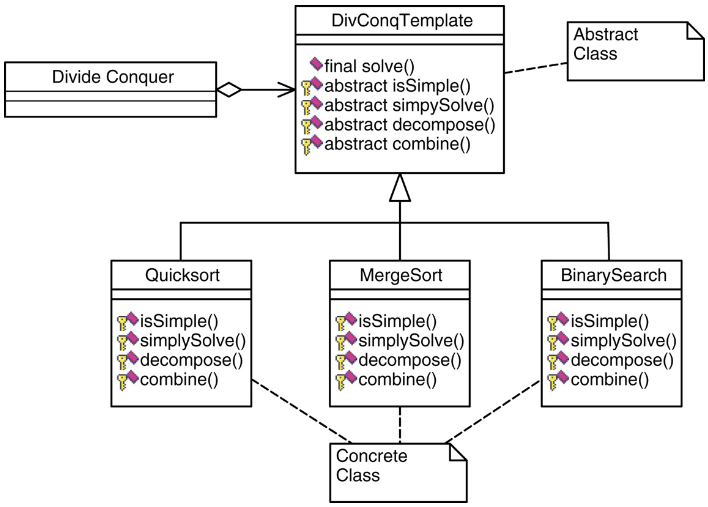
\includegraphics{images/dp_templatemethod_divide.png} 
   \caption{The generic schema of a Divide-and-Conquer \textit{Template Method} designed Framework, with the concrete implementations for various sorting algorithms.}
   \label{fig:dp_templatemethod_code}
\end{figure}

\subsection{Strategy design pattern}
Another one of the behavioural pattern of the \textit{Gang of Four};
Its intent is to allow to select (part of) an algorithm at runtime, leading the client to use an object implementing the interface and
invoking methods of the interface for the hot spots of the
algorithm.

\begin{figure}[htbp]
   \centering
   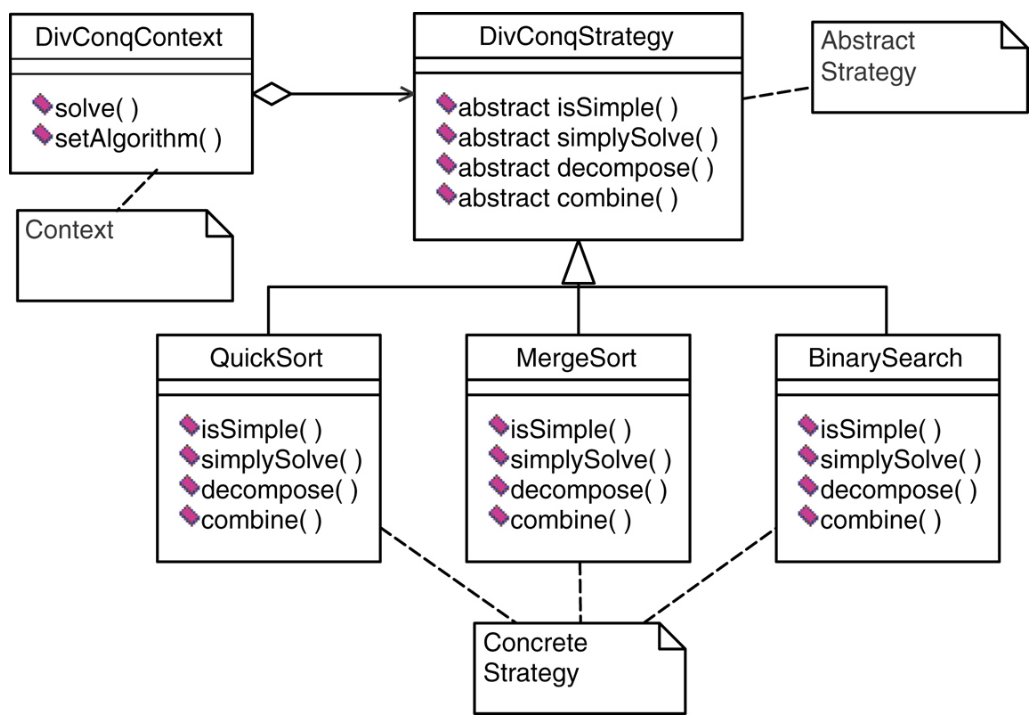
\includegraphics{images/strategyUML.png}
   \caption{Strataegy UML Class Diagram}
   \label{fig:strategyUML}
\end{figure}
\newpage
\subsubsection{Applying the \textit{Separation Principle}}
   The client delegates the hot spots to an object implementing the strategy.
   The implementations of \lstinline|DivCongStrategy| are similar to the previous case.
   
   \begin{lstlisting}
      public final class DivConqContext {
         public DivConqContext(DivCongStrategy dc) { this.dc = dc; }
         
         public Solution solve (Problem p) {
             Problem[] pp;
            if (dc.isSimple(p)) { return dc.simplySolve(p); }
            else { pp = dc.decompose(p); }
            Solution[] ss = new Solution[pp.length];
            for (int i = 0; i < pp.length; i++)
               {  ss[i] = solve(pp[i]); }
            return dc.combine(p, ss);
         }
         
         private DivCongStrategy dc;
         public void setAlgorithm(DivCongStrategy dc) { this.dc = dc;}
      
      }
\end{lstlisting}

\begin{figure}[htbp]
   \centering
   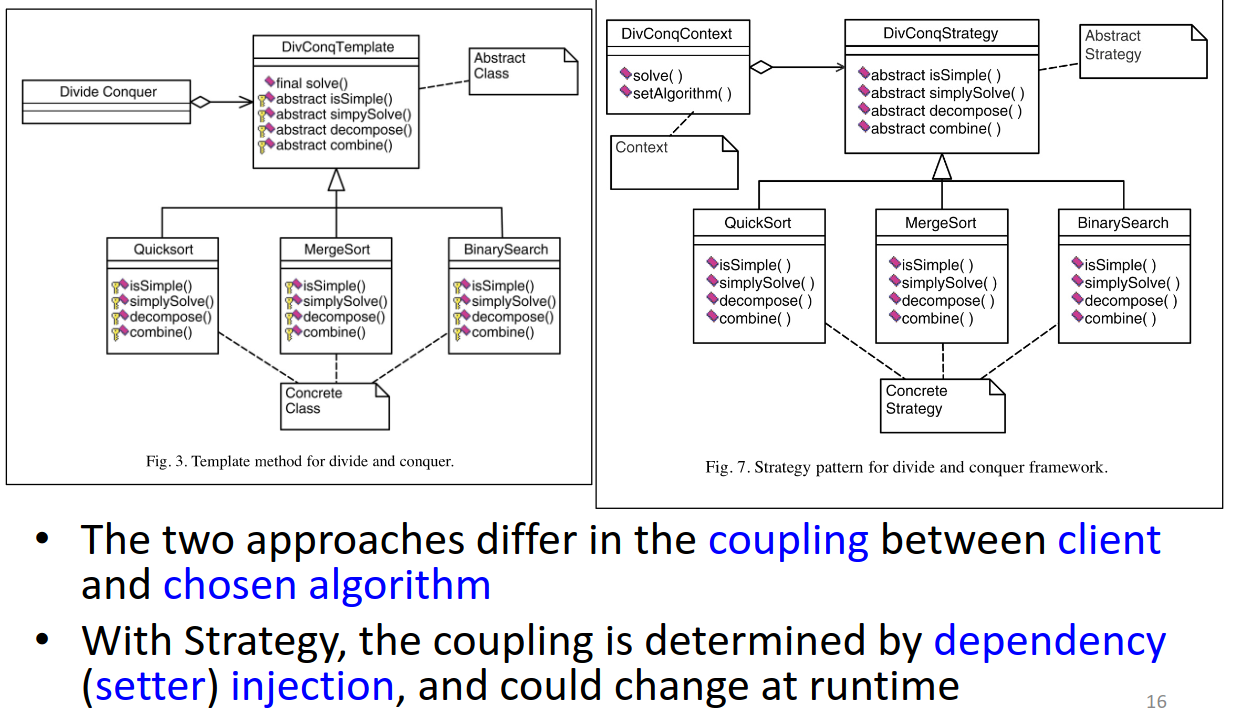
\includegraphics{images/dp_comparison.png}
   \caption{Comparison between the two pattern's schemas}
   \label{fig:dp_comparison}
\end{figure}

\section{Development by generalization}

Recalling what said earlier, we try to address:
\begin{center}
   \textit{Learning to analyze a potential software \textbf{family}, identifying its
   possible common and variable aspects, and evaluating
   alternative framework architectures. Framework design involves
   incrementally \textbf{evolving} a design rather than discovering it in one
   single step}
\end{center}

Where the \emph{evolution} consists of examining \textbf{existing designs} for family members, identifying the \textbf{frozen} and \textbf{hot spots} of the family, and ultimately \textbf{generalizing} the program structure to enable \textit{code reusing} for frozen spots and
multiple \textit{different implementations} for each hot spot.

\ul{In the slides} there is an example based on binary tree traversals, with a discussion on each generalization step.

\begin{figure}[htbp]
   \centering
   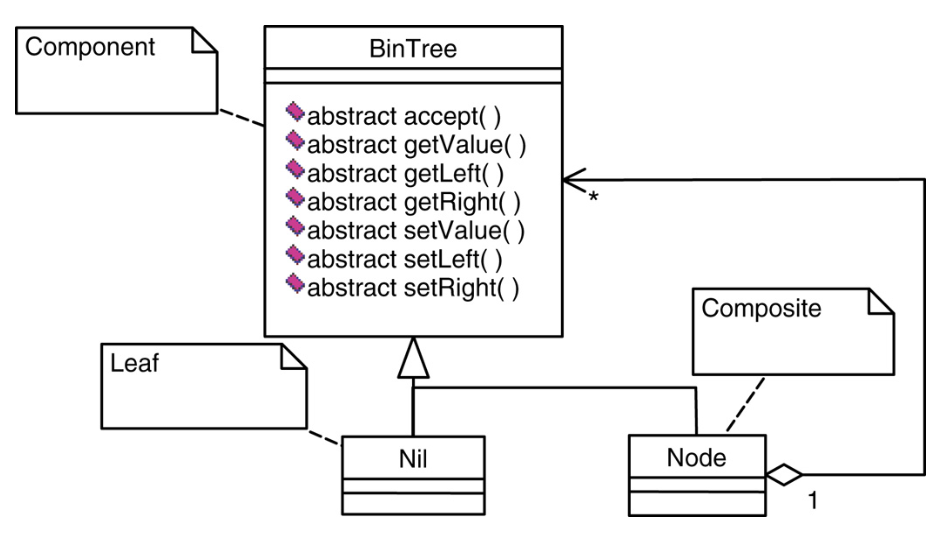
\includegraphics{images/bintree_composite.png}
   \caption{Binary tree using the Composite design pattern}
   \label{fig:}
\end{figure}

\subsection{Identifying Frozen and Hot spots}
\textbf{Frozen Spots}, which are fixed for the whole family:
\begin{enumerate}
   \item The structure of the tree, as defined by the
   BinTree hierarchy
   \item A traversal accesses every element of the tree
   once, but it can stop before completing
   \item A traversal performs one or more visit actions
   accessing an element of the tree
   \note{
      meaning that there may be different and multiple actions after visiting a node,
      since it may represent the end of a left subtree visit, a right subtree visit or a root.}
\end{enumerate}

{Let's identify possible \textbf{Hot Spots}, which have to be fixed in each element of the family.\ns
\begin{enumerate}
   \item Variability in the visit operation’s \textbf{action}:
   a function of the current node’s value and the accumulated result
   \item Variability in \textbf{ordering} of the visit \textit{action} with respect to subtree traversals;
   Should support \textit{preorder},
   \textit{postorder}, \textit{in-order}, and their combination.
   \item Variability in the \textbf{tree navigation} technique. 
   Should support any access order.
   \note{not only left-to-right, depth-first, total traversals}
\end{enumerate}}

\section{Visitor Pattern}
\begin{paracol}{2}
   \colfill
   The \textbf{Visitor} pattern guarantees \textit{separation} between algorithm
   and data structure.
   \nl

   The data structure can be made of different types of components (\textit{ConcreteElements}), and each component implements an
   \lstinline|accept(Visitor)| method.
   The \lstinline|Visitor| defines one visit method
   for each type, including the navigation logic in itself.
   At each step, the correct visit method
   is selected by \textbf{overloading}.
   \colfill
   \switchcolumn

   \begin{figure}[htbp]
      \centering
      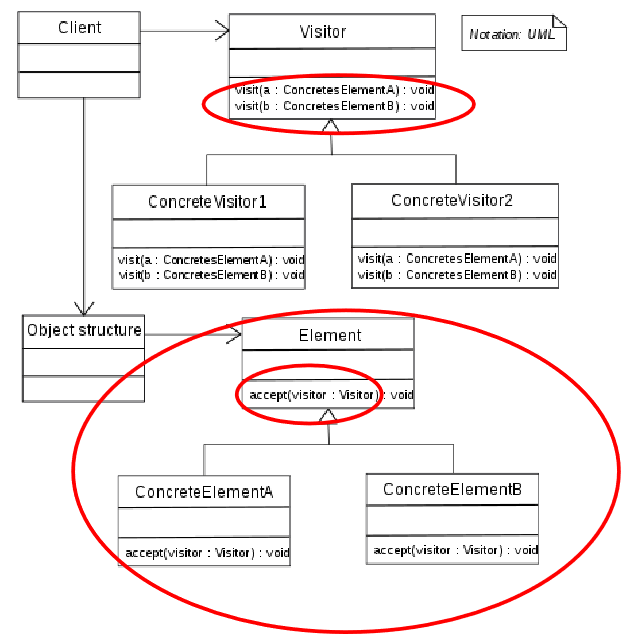
\includegraphics[width=0.9\columnwidth]{images/visitorpattern_uml.png}
      \caption{Visitor Pattern UML generic Diagram}
      \label{fig:visitorpattern_uml}
   \end{figure}
\end{paracol}

Even if in the \textit{Visitor} pattern, as in the \textit{Template Method} pattern, an abstract class is defined and later implemented by subclasses which provide concrete behaviour,
in the \textit{Visitor} pattern such classes are \textit{\textbf{intended}} to be used directly by \textit{clients},
while in the \textit{Template Method} pattern they are \textit{\textbf{intended}} to be called by the \textit{Frozen Spots} inside the abstract class itself, not by \textit{clients}.

\begin{figure}[htbp]
   \centering
   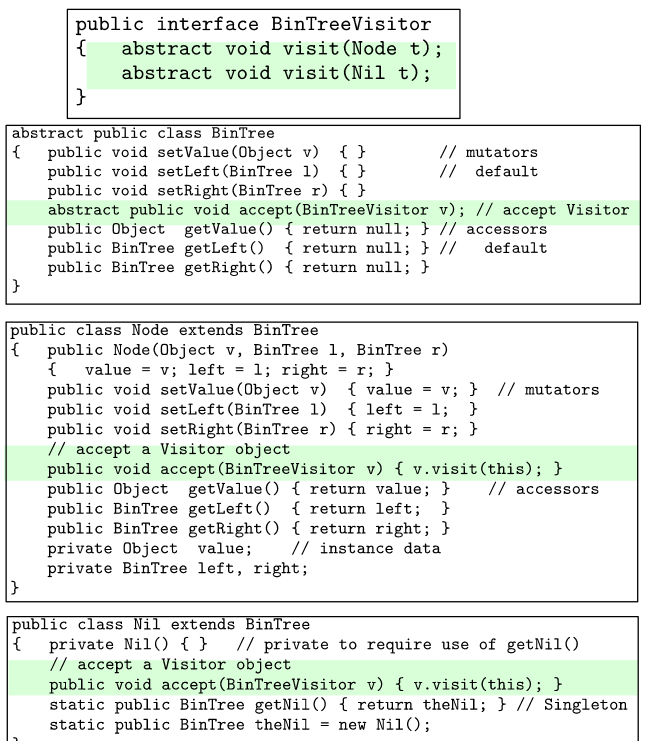
\includegraphics{images/visitorpattern_treecode.png}
   \caption{Visitor Pattern applied to the BinTree visit}
   \label{fig:visitorpattern_treecode}
\end{figure}
\subsection{Wrap Up and Comparison}

The \textbf{Visitor} Pattern
consists of ``Visitees'' or ``Hosts'' and ``Visitors''. Hosts are objects within an object tree, and Visitors contain operations to be performed on these Hosts.

Hosts expose an \texttt{Accept()} method, which takes a Visitor object, and Visitors expose a \texttt{Visit()} method which has an overload for each Host. When the \texttt{Accept()} method is called on the Host, and a Visitor passed, a \texttt{Visit()} method is called on the visitor.

Using this pattern, \ul{operations} become \textit{Double Dispatch},\ul{ meaning they are executed based on two classes: the Host and the Visitor}.
\nl

The \textbf{Strategy} Pattern consists of a ``Context'' and a ``Strategy''. Contexts are \st{objects within a tree} related classes, and a Strategy is a class containing a series of operations to be used by the Contexts.

Strategy provides an interface of which Context objects are aware. When a Context object is created, a Strategy is also created (if not static) and given to the Context. Operations can then be selected from the selected Strategy as desired.
\chapter{TLAV - Thinking Like a Vertex}

MapReduce + HDFS is a solution for many BigData problems, as it allows for processing large amounts of data in a distributed manner. However, it is not the best solution for all use cases, as it has some limitations, such as high latency and lack of real-time processing capabilities.

\note{Recall that HDFS is a distributed file system that allows for storing large amounts of data across multiple machines.}

\section{Spark SQL}
Spark SQL allows to execute SQL queries, which are translated into Spark jobs (more precisely as \textit{actions} and \textit{transformations}). It is built on top of the Spark Core, and provides a more user-friendly interface for working with data.
The result is yielded as a DataFrame, which is a distributed collection of data organized into named columns.

\subsection{Structured Streaming}
The key idea in structured streaming is to treat a live stream as if it were a table that is being continuously appended. This allows for writing SQL queries that process the data in real-time, and to get the results as soon as new data arrives.


\chapter{RUST}
\textbf{Rust} is a general purpose, system programming language
with a focus on safety, especially \textbf{safe concurrency},
supporting both \textit{functional} and \textit{imperative} paradigms.
Its main goal is to \textit{ensure \underline{safety} without penalizing \underline{efficiency}}.\\
\texttt{C/C++} provide more control but less safety, while \texttt{Python/Haskell} provide less control but more safety.
\textbf{Rust} aims to get the best of both worlds, providing both \textbf{control} and \textbf{safety}.

Despite its syntax resemblance to C/C++, in a deeper sense Rust is closer to the ML family languages;
in fact almost every part of a function body is an expression, include \texttt{if-then-else} constructs, which returns a value.

\section{Key Points}
Rust, similarly to C, compilates to \textbf{object code} for bare-metal performance,
but it supports \textbf{memory safety}:
programs can \textit{dereference} only previously allocated pointers that have
not been freed, and \textit{out-of-bound} array accesses not allowed;
Besides, the \textbf{overhead} introduced is very low, since it's the \textit{compiler} which checks that memory safety rules are followed,
and there's \textit{\underline{no} garbage collection}, so zero-cost abstraction in managing memory.\\
This is achieved through and \textbf{advanced type system} and three key concepts to prevent memory corruption:
\begin{enumerate}
   \item Ownership
   \item Borrowing
   \item Lifetime
\end{enumerate}

Again, Rust is designed to be \textbf{memory safe} even in the presence
of concurrency, and guarantees the following properties \textbf{statically}, meaning that
if the program \textit{compiles} it will \textit{never manifest a violation} of these properties: 
\begin{itemize}
   \item No \texttt{null} pointers\\
   $longrightarrow$ accessing a variable which does not hold a value
   \item No dangling pointers\\
   $longrightarrow$ Pointers to invalid memory location
   \begin{itemize}
      \item Pointers to explicitly deallocated objects;
      \item Pointers to locations beyond the end of an array;
      \item Pointers to objects allocated on the stack;
   \end{itemize}
   \item No double frees\\
   $longrightarrow$ A memory location in the heap is reclaimed twice
   \item No data races\\
   $longrightarrow$ unpredictable results in concurrent computations
   \item No iterator invalidation
\end{itemize}

\section{\texttt{null} and Primitive types in Rust}
A \texttt{null} value does \textbf{not} exist in Rust, so in some way it must address the problem of accessing a variable which does not hold a value.\\
Data values can only be initialized through a fixed set of
forms, requiring their inputs to be already initialized, and if 
any branch of code fails to assign a
value to the variable, we get a \textbf{compile time error}.
\note{Static/global variables must be initialized at declaration
time.}
\lstset{language=Rust}
\textit{Nullable} types, are managed with a generic \lstinline|Option<T>|, playing
the role of Haskell’s \texttt{Maybe} or Java’s \texttt{Optional}
\begin{lstlisting}
   enum std::option::Option<T> {
      None,
      Some(T)
   }
\end{lstlisting}

\subsection{Primitive Types}
\begin{lstlisting}[caption={Rust primitive types}]
   // Numeric types:
   i8 / i16 / i32 / i64 / isize
   u8 / u16 / u32 / u64 / usize
   f32 / f64
   
   bool
   char // (4-byte unicode)
\end{lstlisting}
\begin{itemize}
\item \textbf{Type inference} for variables declarations with let
\item \textbf{No overloading} for literals: type annotations to disambiguate
\item \textbf{Tuples} like in Haskell
\item \textbf{Arrays} with fixed length. 
\note{\textit{out-of-bound} access is checked at \textbf{runtime},
but it's just a single comparison, its overhead is negligible}
\end{itemize}

\section{Memory Management}
As usual, Rust uses a \textbf{stack} of activation records, and a \textbf{heap} for dynamically allocated data structures.

The user is forced to be \textit{aware of where} the data are stored: 
there is no \textbf{implicit boxing}\footnote{Act of \textit{boxing} an \texttt{int} in \texttt{Integer}, or extracting an \textit{int} from \textit{Integer}}.

\begin{lstlisting}
   fn main() {
      let x = 3; // 'let' allocates a variable on the stack
      let y = Box::new(3); // y is a reference to 3 on the heap
      println!("x == y is {}", x == *y); // "x == y is true"
      }
\end{lstlisting}

To avoid the overhead of a Garbage collection mechanism and the possible subtle errors introduced a programmer to whom memory management is delegated, Rust provides \textit{deterministic management of
resources}, with very low overhead, using \textbf{RAII} (\textit{\underline{R}esource \underline{A}cquisition \underline{I}s \underline{I}nitialization}).
\nl

By \textit{default}, Rust variables are \textbf{immutable}, and their usage is statically checked by the compiler.
\lstinline|mut| is used to declare a resource as mutable.
\begin{paracol}{2}
\begin{lstlisting}[caption={Compilation \textit{error}}]
   fn main() {
      let a: i32 = 0;
      a = a + 1;
      println!("a == {}", a);
   }
\end{lstlisting}
\switchcolumn
\begin{lstlisting}[caption={Compilation \checkmark}]
   fn main() {
      let mut a: i32 = 0;
      a = a + 1;
      println!("a == {}", a);
   }
\end{lstlisting}
\end{paracol}

The \textit{Resource Acquisition Is Initialization} (\textbf{RAII}) programming idiom states that Resource \textit{allocation} is done during object
\textit{initialization}, by the constructor, while resource \textit{deallocation}
(\textbf{release}) is done during object destruction (specifically
\textbf{finalization}), by the destructor.

\subsection{Ownership}

This approached is adopted in modern \texttt{C++}: 
small objects are allocated on \textit{stack},
while larger resources are on the \textit{heap} {--}or elsewhere{--} and are \textbf{owned} by an object on the \textit{stack},
who is responsible for \textit{releasing} the resource in its destructor.\\
Each resource has a \textbf{unique owner}.

Rust supports RAII in a \textit{strict} way through an \textbf{ownership system}, based on the concepts of \textit{\underline{ownership}} and \textit{\underline{borrowing}}.
\labelitemize{\textit{Ownership}}{
   \begin{enumerate}[label=\texttt{O\arabic*} - , left=1em]
      \item Every value is \textit{owned} by a variable, identified by a name (possiby a path);
      \item Each value has \textit{at most \underline{one owner} at a \underline{time}};
      \item When the owner goes \textit{out-of-scope}, the
      value is \textit{reclaimed} / destroyed.
   \end{enumerate}
}

By default, an assignment between variables has
a \textbf{\underline{move} semantics}:
the ownership is moved from the RHS to the LHS 
\begin{lstlisting}
   fn main() {
      let x = Box::new(3);
      let _y = x; // underscore to avoid 'unused' warning
      println!("x = {}", x); // error!
      }
\end{lstlisting}
For primitive types and types implementing the \textbf{Copy
trait}, assignment has a \textbf{\underline{copy} semantics};
\begin{center}
   Here \texttt{O2} is satisfied because a new value is created
\end{center}
\begin{paracol}{2}
   \begin{lstlisting}
      fn main() {
         let x = 3;
         let _y = x;
         println!("x = {:?}", x); // OK
      }
   \end{lstlisting}
   
   \switchcolumn

   \begin{lstlisting}
      fn main() {
         let x = Option::Some(3);
         let _y = x;
         println!("x = {:?}", x); // OK
      }
   \end{lstlisting}
\end{paracol}

The same move semantics apply also for parameter passing:
Any value passed to the function will be reclaimed
when it returns, as the formal parameters gets out of
scope;
only returned values can survive.
\note{
   tuples allow to return more
}
\begin{lstlisting}
   struct Dummy { a: i32, b: i32 }
   fn foo() {
      let mut res = Box::new(Dummy {
         a: 0,
         b: 0
   });
   take(res);
   println!("res.a = {}", res.a); \\ compilation error
   }
   fn take(arg: Box<Dummy>) {...}
\end{lstlisting}

When invoking \lstinline|take(res)| the ownership of \lstinline|Dummy| is moved from \lstinline|res| to \lstinline|arg|:
when \texttt{take()} returns \lstinline|arg| goes out of scope, so the resource gets freed automatically, making it no longer usable in \lstinline|println|:
this result in a \textbf{compilation error}.
To use again the resource, we would have to make take return it, i.e. \lstinline|res = take(res)|.

This looks rather limiting, but allows to completely avoid the \textit{Double-free} problem:
memory is freed automatically
when the owner goes out of scope, and by rule \texttt{O2}, each value has only one owner.
\note{Rust does not allow explicit memory allocation}

\subsection{Borrowing}
Since Ownership rules in some case may be too restrictive, \textbf{borrowing} is introduced: a resource can be \textit{borrowed} from its owner via
assignment or parameter passing.
To guarantee memory safety, borrowing rules ensure
that \textit{aliasing}\footnote{Both the owner and the borrower can access the resource.
More generally indicates that there are multiple ways to access a resource on the heap.} and \textit{mutability cannot \textbf{coexist}}.\\
Values can be passed
\begin{enumerate}
   \item by immutable reference $\longrightarrow$ \lstinline|x = &y|
   \item by mutable reference $\longrightarrow$ \lstinline|x = &mut y|
   \item or by value $\longrightarrow$ \lstinline|x = y|
\end{enumerate}

\labelitemize{\textit{Borrowing}}{
\begin{enumerate}[label=\texttt{O\arabic*} - , left=1em]
   \label{enum:borrowing_rules}
   \item[] \note{\qquad About mutable and immutable references:}
   \item At most \textbf{one} \textit{mutable} reference to a resource can exist at any time
   \item If there is a \textit{mutable} reference, \textbf{no} \textit{immutable} references can exist
   \item If there is \textbf{no}\textit{ mutable} reference,\textbf{several}
   \textit{immutable} references to the same resource can exist

   \item[] \note{\qquad During borrowing, ownership is reduced or
   suspended:}
   \item Owner \textit{cannot} free or \textbf{mutate} its resource while it is \textit{immutably borrowed}
   \item Owner \textit{cannot} even \textbf{read} its resource while it is \textit{mutably borrowed}
\end{enumerate}
}

\subsection{Strings}
\labelitemize{\textit{String types}}{
   \begin{enumerate}
      \item \lstinline|String|
      does not require to know the length at compilation
      time, thus allocated on the \textit{heap}.
      \item \lstinline|&str|
      size must be known statically, allocated on the \textit{stack}.
   \end{enumerate}
   }
\note{
   Method \lstinline|String::from()| allocates memory on the heap: it takes an argument of type \lstinline|&str| and returns a \lstinline|String|.
}

A String object has three components:
\begin{enumerate}
   \item a reference to the heap location containing the character sequence
   \item capacity (unsigned integer)
   \item length (unsigned integer)
\end{enumerate}
\lstinline|String| does not implement \lstinline|Copy|, thus assignment is subject to move semantics;
assignment creates a copy of length, capacity and reference,
but not of the char sequence in the heap.

\subsection{Lifetime}
A \textbf{lifetime} is a construct that the borrow checker uses to ensure the validity of the \textit{borrowing rules} \ref{enum:borrowing_rules}.
Lifetimes are associated with each individual ownership
and borrowing: 
a lifetime \textit{begins} when the ownership starts, and \textit{ends}
when it is moved / destroyed, 
while for borrowings, it ends where the borrowed value is
accessed the last time.

Lifetimes are mostly \textit{inferred},
but sometimes they must be made explicit using the same syntax of generics.
Using lifetimes, the compiler checks the validity of the
rules of ownership and borrowing in the expected way;
in particular, it ensures that {--}the \textit{owner} of{--} every
borrowed variable/reference has a lifetime that is longer
than the borrower \texttt{[B4,B5]}.
\nl

Borrowed (reference) formal parameters (arguments, return value) of a function have a
lifetime, and  
if borrowed values are returned, each \textit{must} have a lifetime.\\
The compiled tries to infer output lifetimes according to the following rules, but when not sufficient explicit lifetimes are necessary:
\labelitemize{\textit{Lifetime}}{
   \begin{enumerate}[label=\texttt{R\arabic*} - , left=1em]
      \item The lifetimes of the borrowed paramers are, by default, all \textbf{distinct}
      \item If there is \underline{exactly} \textbf{one input} lifetime, it will be assigned to \textbf{each
      output} lifetime
      \item If a method has \textbf{more than one input} lifetime, \textit{but} \textbf{one} of them is
      \lstinline|&self| or \lstinline|&mut self|, then this lifetime is assigned to \textbf{all output} lifetimes
   \end{enumerate}
}

\begin{lstlisting}
   fn longest(s1: &str, s2: &str) -> &str { //does not compile
      if s1.len() > s2.len() { s1 }
      else { s2 }
   }
\end{lstlisting}
Here the lifetime of the parameters depends on whether \lstinline|s1| or \lstinline|s2| is returned,
so the compiler cannot infer the lifetime of the output parameters;
hence, an \textbf{explicitly named lifetime} for input parameters is requires, as in the following snippet.
\begin{lstlisting}
   fn longest<'a>(s1: &'a str, s2: &'a str) -> &'a str {
      if s1.len() > s2.len() { s1 }
      else { s2 }
\end{lstlisting}
\newpage

\section{More on Types}
\subsection{Enums}
\begin{paracol}{2}
   \begin{lstlisting}
enum RetInt {
      Fail(u32),
      Succ(u32)
   }
fn foo_may_fail(arg: u32) -> RetInt {
      let fail = false;
      let errno: u32;
      let result: u32;
      ...
      if fail {
            RetInt::Fail(errno)
         } else {
            RetInt::Succ(result)
         }
   }
\end{lstlisting}
\switchcolumn
\begin{lstlisting}
#[derive(Debug)] // needed to print
enum Tree<T> {
   Empty,
   Node(T, Box<Tree<T>>, Box<Tree<T>>)
}

fn main() {
   let tree = Tree::Node(
      42,
      Box::new(Tree::Node(
         0,
         Box::new(Tree::Empty),
         Box::new(Tree::Empty)
      )),
      Box::new(Tree::Empty));
   println!("{:?}", tree);
   //>Node(42, Node(0, Empty, Empty), Empty)
}
\end{lstlisting}
   \lstinline|println!("{:?}", tree);| indicates to print \lstinline|tree| in \textit{"debug mode"}.
\end{paracol}

\subsection{Pattern Matching}
\begin{lstlisting}
   let x = 5; // try others...
   match x {
      1              => println!("one"),
      2              => println!("two"),
      3|4            => println!("three or four"),
      5..=10         => println!("five to ten"),
      e @ 11..=20    => println!("{}", e),
      i32::MIN..=0   => println!("less than zero"),
      21..           => println!("large"),
      _              => println!("???"),
   }
\end{lstlisting}


\subsection{Classes}
Rust is \textbf{not} \textit{Object Oriented} and there is \textbf{no inheritance}, instead it pushes for composition over inheritance.

\begin{lstlisting}
#[derive(Debug)]
struct Rectangle { // class
      width: u32, // instance variable
      height: u32,
   }
impl Rectangle { // methods
      fn area(&self) -> u32 { // first argument is this
            self.width * self.height
            // self.width = 20; // <- illegal, self is immutable
         }
   }
fn main() {
      let rect1 = Rectangle {
            width: 30,
            height: 50,
         };
      println!(
      "The area of the rectangle is {} square pixels.", rect1.area()
      );
   }
\end{lstlisting}

\subsection{Traits}
\textbf{Traits} are equivalent to \textit{Type Classes} in Haskell and to \textit{Concepts} in
C++20, similar to Interfaces in Java.
A trait can include \textit{abstract} and \textit{concrete} (default)
\textbf{methods}, but \underline{not} fields or variables.
A struct can implement a trait providing an
implementation for at least its abstract methods
\begin{lstlisting}
   impl <TraitName> for <StructName>{ ... }
\end{lstlisting}

The \lstinline|#[derive]| clause can be used {--}if possible{--} to derive
automatically an implementation of a trait.

Rust supports \textbf{bounded universal explicit polymorphism}
with \textbf{generics}, as in Java, where bounds are one or
more traits. 
\chapter{System Design View}


\section{Thesis = Fuzzing Hardware}
Baiardi is interested in \textit{Fuzzing Hardware},
he would like to do a thesis on such topic.

\section{System View}
\textbf{System view} is a perspective aiming to consider \textit{design rules} and consequentently \textit{vulnerabilities},
focusing on wrong design choices rather than
implementation error.
A set of design rules is used to determine the \textit{optimal} set of \textbf{controls} for a system, where \textit{optimal} indicates the smallest (i.e. \textit{cheapest} \smiley)set of controls to achieve the required robustness.\\
It is important to understand whether the optimal set of controls as imposed
by the design rules is compatible with the required performance,
and from this point of view we can define a \textbf{vulnerability} as a \textit{violation} of system design rules.

\subsection{Robustness agains Vulnerabilities}
Thus, in this scenario, designing a system means finding an acceptable \textbf{tradeoff} between \textit{design rules} and \textit{vulnerabilities}.

All the modules in an ideal system satisfy the design rules,and such ideal system is the asymptote of a sequence of distinct systems each applying more controls than the previous one as required by the design rules.\\
Any difference between the ideal system and the one being
created/under analysis may be considered as a \textbf{vulnerability},
but to decide if it is an actual vulnerability we consider the \textbf{context}
and the \textbf{cost} of the control against its usefulness.
\nl

Some differences between the ideal system and the current one cannot be avoided, supponsing some rules have been violated due to {---}possibly basic{---} performance requirements.
Other violations (i.e. \textit{missing controls}) instead may be unrelated to
performance, hence they should be fixed.\\
The key strategy to discover vulnerabilities evaluates the cost of
missing controls and compares it against
\begin{itemize}
   \item the required final \textit{performance}
   \item the \textit{risk} ($\mathcal{P}(intrusion) *impact$) due to the missing control
\end{itemize}
In a whole-system comprehensive view it is important to check \textbf{compensative controls}, i.e.
a missing control in a module may be compensated by a
control in another one.

\section{Saltzer \& Schroeder}
\labelitemize{S\&S Design Principles}{
   \begin{enumerate}
      \item \textbf{Economy of Mechanism}\\
      The protection mechanism should have a \textit{simple} and small design.
      \item \textbf{Fail-safe Defaults}\\
      The protection mechanism should \textit{deny} access by \textit{default}, and grant access
      only when explicit permission exists.
      \item \textbf{Complete Mediation}\\
      The protection mechanism should check \textit{every access} to every object.
      \note{
         Rather expensive this is the reason is one of the most hard to satisfy.
      }
      \item \textbf{Open Design}\\
      Protection mechanism should not depend on attackers being ignorant of
      its \textit{design} to successfully secure the system. 
      But may be based on the attacker's ignorance of
      specific information such as passwords or cipher keys.

      \emph{
         \color{darkgray}"An attacker who learns the key learns nothing that helps them break any message
      encrypted with a different key. That’s the essence of Kerkhoff’s principle: that
      systems should be designed that way."}
      
      \note{
         However, you should publish information on your system design \emph{iff} it results in a
         useful \textbf{peer review}.
         }
      \item \textbf{Separation of Privilege}\\
      The protection mechanism should grant access based on \textit{more than
      one piece} of information, e.g. \textit{two keys} for a safe.
      \item \textbf{Least Privilege}\\
      The protection mechanism should force every process to operate with
      the \textit{minimum privileges} needed to perform its task.
      \item \textbf{Least Common Mechanism}\\
      The protection mechanism should be shared as little as possible among users.
      \item \textbf{Psychological Acceptability}\\
      The protection mechanism should be easy to use (at least as easy as not using it).

      \note{
         Before introducing the last two principles, Saltzer and Schroeder state two things:
         \begin{itemize}
            \item Analysis of traditional physical security systems has suggested two further design principles which, unfortunately,
            apply only \textit{imperfectly} to computer systems
            \item The principles apply both to a system and to the \textit{mechanisms} we introduce to secure the system
         \end{itemize}
      }

      \item \textbf{Principle of Work Factor}\\
      Compare the cost of circumventing the mechanism against the resources of a potential attacker.
      \item \textbf{Compromise Recording}\\
      Mechanisms that reliably record a compromise of information may replace more elaborate ones that completely prevent loss.\\
      In other words,
      if you cannot be robust be aware you may be attacked and be resilient.
   \end{enumerate}
}
\subsection{Economy of mechanisms}
\begin{center}
   \textit{Keep the design as simple and small as possible}
   \note{
      \textit{KISS} rule $\longrightarrow$ \textit{\underline{K}eep \underline{I}t \underline{S}imple, \underline{S}tupid}
   }
\end{center}

\textbf{Simple} implies that less things can go wrong and when bugs occur, they are easier to find, understand and fix.
Vulns are proportional to the complexity of a mechanism and the code implementing it.
% = cyclomatic number to predict software bugs
When needed, complexity can be achieved by \textbf{composition} of simpler modules, and might be preferreable to building a single more comprehensive yet complex module.\\
\subsection{Designing Operating Systems}
\textbf{OS Hardening} is an approach embodying this principle:
it consists in removing useless OS functionalities for applications
of interest.\\
With respect to kernel, there are two approaches which aim to reduce complexity:
\begin{itemize}
   \item \textbf{Microkernel}\\
   Avoid the implementation of complex functions in the kernel,
   stick only to \textbf{basic} ones such as inter-process communication and basic memory management,
   possibly making room for a \textit{modular} design.
   \note{Unix and Windows do not follow this approach,
   which is instead adopted by QNX and MINIX, for instance}
   \item \textbf{Esokernel}\\
   Focus on providing \textbf{minimal abstractions} to applications and exposing as much hardware functionality as possible to applications,
   creating astrong \textbf{integration} between the OS kernel and the
   applications not only violates modularity principles
   but helps the spreading of errors.
\end{itemize}

\subsection{Wrapping Up}
\begin{itemize}
   \color{darkgreen}
   \item \textbf{Simplify} the interface
   \item Complex operations should be implemented by \textbf{composing}
   simple operations

\end{itemize}
\begin{itemize}
   \color{darkred}
   \item If most of the operations are rather complex (and hence
   powerful), we may be forced to enable a user to invoke a
   powerful operation just because the simple one it needs is
   missing
   \item Hence, users will apply complex operations even to
   implement simple operations and this increases their rights
   (related to the least privilege principle)
\end{itemize}

\subsection{Fail-safe and Intel \texttt{CSME}}
\begin{center}
   \textit{Base access decisions on permission rather than
   exclusion}
\end{center}
Fail-safe related vulnerabilities are fascinating, and may be \textit{non-trivial} to abuse.
Some aspects cannot be fixed without replacing the \textit{silicon}, but only \textit{mitigated}.

Fail-safe is related to a \textit{design flaw} baked into millions of Intel chipsets:
the problem revolves around cryptographic keys that, if obtained by an attacker,
can be used to break the \textbf{root of trust} in a system.

\subsubsection{Intel Countermeasure}
Buried deep inside modern Intel chipsets there is the \textbf{Converged
Security and Manageability Engine} (\texttt{CSME}),
which is a miniature computer within a computer with its own CPU, RAM, code in a boot ROM, and with the capability to access the rest of the machine.

Currently, the \texttt{CSME}'s CPU core is 486-based, and its software is
derived from the free \textbf{microkernel} operating system \texttt{MINIX}.
\note{
   You can
   find a deep dive into the technology behind it all, sometime known
   as the Minute IA System Agent.
}
The \texttt{CSME} is digital janitor, working behind the scenes, below
operating system, hypervisor, and firmware, performing lots of
crucial low-level tasks.
\begin{itemize}
   \item Bringing up the computer, controlling power levels,
   \item Starting the main processor chips
   \item Verifying and booting motherboard firmware, and providing
   cryptographic functions.
   \item The engine is the first thing to run when a machine is switched on.
\end{itemize}

\paragraph{Possible Flaw}
One of the first things the \texttt{CSME} protects is its \textbf{own built-in RAM} so that other hardware and software module cannot interfere.
However, these protections are disabled by default, there is a tiny timing gap between a system turning on and the \texttt{CSME} executing the code
in its boot ROM that installs such protections in the form of input-
output memory-management unit page tables.
During that timing gap, other hardware - physically attached or
present on the motherboard can fire off a DMA transfer into the
\texttt{CSME}’s private RAM to overwrite variables and pointers and hijack
its execution. 
At that point, the \texttt{CSME} can be controlled for
malicious purposes, all out of view of the software running above it.

Clearly this a strong \textbf{race condition}, but still possible.

\subsection{Complete Mediation}
\begin{center}
   \textit{Every access to every object must be checked for authority}
\end{center}

This is the most crucial principle when considering performance,
since verbatim applying it would be very impactful on the system's performance.

Usually access to object is done only once on the first time,
but this leads to possible unauthorized accesses if permissions change later on.\\
Performance enhancements are achieved by caching results of
authority checks,
but they should be examined skeptically,
to avoid the above mentioned unpleasant situation.
Every uncontrolled operation that is a potential vulnerability as it may be invoked without proper rights.

\subsubsection{Fail-safe integration}
If \textbf{both} principles are \textbf{satisfied} the system starts in a secure state and,
provided that the security kernel is correct, further on only secure transictions are enabled.
In other words, it is possible to prove security correctness using an induction approach to determine reachable states.\\
\textit{Fail-safe} plays a key role since it makes valid the base case for the induction, it acts as a "starting point".
If fail-safe default does not hold then no induction is possible
there is no base case for the induction.

\subsection{Open Design}
\begin{center}
   
   The design should not be secret\\
   or\\
   Security should not depend on the secrecy of
   the design or of the implementation
\end{center}
Popularly misunderstood as
\textit{"source code should be public"} or \textit{"open-source is safer than proprietary"}.

A system \textbf{peer review} is fundamental to discover vulns in
design or implementation.
A \textit{peer review} is review made by \textbf{competent experts} which can discover flaws and vulnerabilities in a system.
So, an open source implementation is useful only if it results in a peer review, and if any peer that discovers a vulnerability communicates it
to the owner.
Instead it is useless and possibly dangerous if there are no peers available to review the code,
or they do not reveal to the owner the discovered vulnerabilities.

\begin{figure}[htbp]
   \centering
   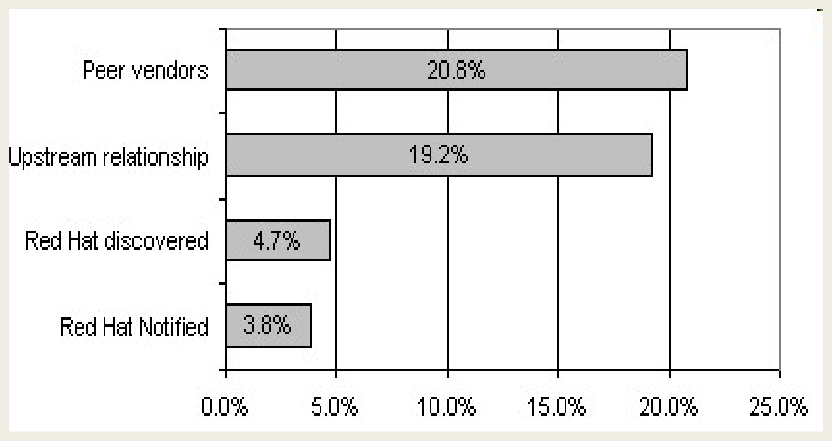
\includegraphics[width=0.45\columnwidth]{images/opendesign_redhat.png}
   \caption{RedHat vulnerabilities}
   \label{fig:opendesign_redhat}
\end{figure}
As an example, consider RedHat's statistics:
as you can see in Fig \ref{fig:opendesign_redhat}, most of the known vulnerabilities were discovered by peers,
not by RedHat's own experts.

\subsection{Separation of Privilege}
\begin{center}
   \textit{Where feasible, a protection mechanism that requires
   two keys to unlock is more \textbf{robust} and \textbf{flexible} than one
   that allows access using a single key}\\
   or\\
   \textit{Require multiple conditions to grant privilege}
\end{center}

\subsubsection{Decomposing}
A complex operation should be decomposed into simpler
operations, 
each enabled by a proper access rights,
both the complex and the simple ones.\\
In this way we can check that the subject owns both
\begin{enumerate}
   \item The right of invoking the complex op (if it still exists)
   \item The right of invoking each simple op
\end{enumerate}

\subsection{Least Privilege}

Every subject should operate using the least set of privileges
necessary to complete its job
or
A subject should be given only those privileges it needs to complete
its task and only for the time to complete it

According to Baiardi, this is the most crucial principle to be kept in mind.
Many intrusion have succeed due to the violation of this principle. 
\labelitemize{\textit{Key Points}}{
   \begin{itemize}
      \item Owning a useless access right is a \textit{vulnerability}
      \item Rights \textit{granted as needed}, \textit{revoked} after being used
      \item The \texttt{AC} matrix is a \textit{highly dynamic} data structure
      \item Rights are \textit{assigned} and \textit{revoked} as the \textit{computation evolves}
   \end{itemize}
}

This principle should be applied even if the security policy is
\textbf{static},
since it defines mostly how rights should be managed \textit{after} being
granted to each subject rather than how they are granted.\\
If, in a given time interval, a subject \textit{does not need} a right
then this right should be revoked and then granted again later on by
updating the \texttt{ACM} to prevent the subject from exploiting the right in such time interval.\\
The right is removed at the beginning and then granted at the
end of the \textit{"not-needing" interval}.

\subsubsection{Protection Domain Switching}
\textbf{Protection Domain Switching} (\texttt{PDS}) consists in updating an \texttt{ACM} row,
making the same subject executed
with \textit{updated rights} in \texttt{ACM}.\\
Note that it is possible to have a \texttt{PDS} without a \textit{context switch}.
The performance overhead introduced by \texttt{PDS} is a function of the
implementation level and the adopted implementation of the
\texttt{ACM} (\textit{Capabilities} vs \texttt{ACL});
When the implementation relies on capabilities revoking a right is not trivial,
delegation and race conditions are involved.

\subsubsection{Small Domain Principle}
An alternative definition of this principle is \textbf{the small
domains principle}, to stress the importance of minimizing the
protection domains $\longrightarrow$ the number of the subject rights $\longrightarrow$ the
\textit{frequency} of the \textit{commutation} of the protection domain.\\
Besides, as the size of the protection domain decreases, it also
decreases the risk of an attack against the considered
subject.\\
If the protection domains are \textit{not small}, then we revoke access
rights when not needed and grant them again when needed, as described before.

\nl
Notice the strong relation between the two last principles
because segmented networks force the reduction of protection
domain and separation of duties enables the implementation of
the least privilege.

\subsubsection{Common implementation}
In the classical solution a \textit{domain switching} occurs when
\begin{enumerate}
   \item A procedure (method) is \textbf{invoked}
   \item A procedure (method) \textbf{returns}
\end{enumerate}

Instead of updating row, creation (\textit{invoke}) and deletion (\textit{return}) are typically preferred.\\
When a procedure is invoked, a new row that defines its
rights is created and gets deleted when the procedure returns.
Rights are paired with the \textbf{instance} of a procedure executed
by (or on behalf of) a subject rather than with the actual procedure
code or with the subject.

The rights in the new row are a function of:
\begin{itemize}
   \item Method private variables
   \item Input parameters
\end{itemize}
The program structure in terms of \textit{classes/methods} defines the
strategy to manage rights granted to the subjects on
program data structures,
allowing automated handling of \texttt{PDS} and 
the programmer to choose the size of each protection
domain.

\subsubsection{Network Programming}
In network programming the least privilege principle is
managed through dynamic communication channels.\\
A server can be designed by introducing a distinct communication
channel for each operation implemented by the server; 
a process is \textbf{connected}\footnote{i.e. can send messages} to the channel
paired with an operation \texttt{Op} {---}{with a service \texttt{S}}{---} when it can
invoke the operation {---}{can access the service}{---};
then process is \textbf{disconnected} from the channel when it can no
longer invoke the operation.

The adoption of dynamic channels \textit{reduces} the \textbf{overhead} to reject a request by implementing in the OS kernel a mechanism to ope and close ports.\\
The overhead \textit{on the server} can be further reduced by \textit{"spreding the news"}
that a message from a given node to a given port of a receiver
can be \textit{dropped} by routers or firewall;
However, this implies a larger overhead on other nodes to update \textit{routing tables} or \textit{firewall rules}.\\
On the other side, if only the final node or, even worse, the final
server can drop messages we offer an opportunity for a
\textbf{DDoS attacks} where a server is overflown by a large number of
requests to be discarded.

\subsubsection{Defence-in-depth and Network Segmentation}
\begin{figure}[htbp]
   \centering
   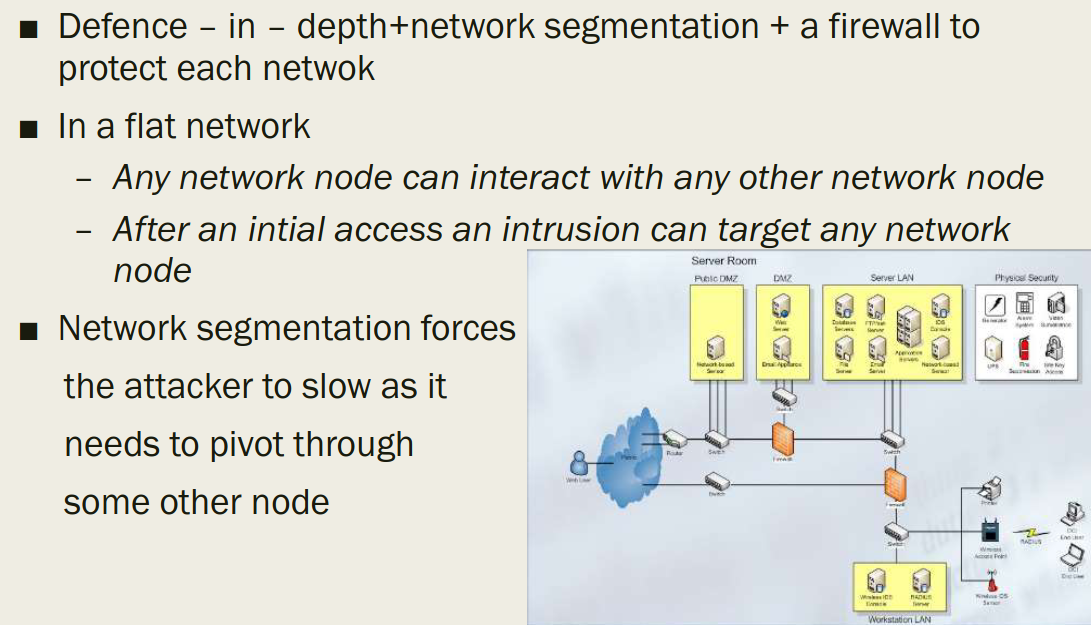
\includegraphics{images/leastprivilege_networkseg.png}\\
   \textbf{Network Segmentation} can be seen as an implementation of \textit{Defence-in-Depth} (Least Privilege key point) when designing system networks.
   \caption{Least Privilege and Network Segmentation}
   \label{fig:leastprivilege_networkseg}
\end{figure}

\subsubsection{ZeroTrust Network}

Recall that the basic idea of \texttt{ZT} is to authenticate both the \textbf{user} and the \textbf{device} exploited by the user to access a \textbf{service};
\note{
   Authenticating a device means searching for the device security status in an inventory to check the vulnerabilities that affect the device and which patches have been applied
}

\begin{figure}[htbp]
   \centering
   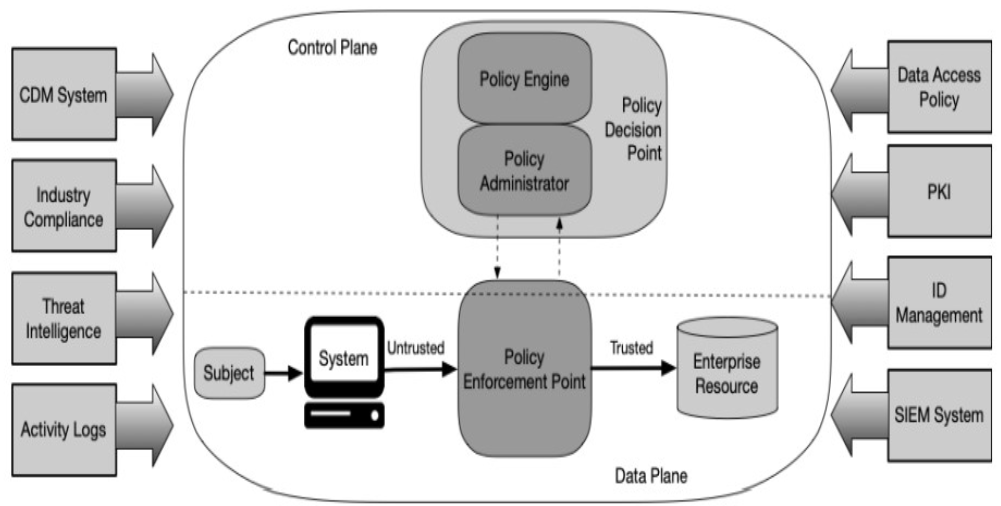
\includegraphics{images/leastprivilege_zerotrust.png}
   \caption{ZeroTrust in Networks to apply \textit{Least Privilege} principle}
   \label{fig:leastprivilege_zerotrust}
\end{figure}

\begin{enumerate}
   \item \textbf{No implicit trust} is granted to assets or user accounts based
   \textit{solely} on their physical or network location (i.e., local area networks versus the internet) or based on asset ownership
   (enterprise or personally owned).
   \item Authentication and authorization (both subject and device) are
   performed \textbf{before} establishing a session to enterprise resources
   \item Zero trust is a response to enterprise network trends that include remote users, "bring your own device" and cloud-based assets
   not located within an enterprise-owned network boundary.
   \item Zero trust protects \textbf{resources} (assets, services, accounts, etc.), \textbf{\textit{not} network segments},
   since the network location in most nowdays infrastructures is no longer the
   prime component to the security posture of the resource.

   \item All data sources and computing services are considered resources
   \item All communication is secured regardless of network location because
   location alone does not imply trust.
   \item Access to individual enterprise resources is granted on a per-session
   basis (no caching). Trust in the requester is evaluated before granting
   access with the least privileges to complete the task.
   \item Access to resources is determined by dynamic policy (= the
   observable client identity, application/ service, and the requesting
   asset) and may include behavioral and environmental attributes.
   \item The enterprise monitors and measures the integrity and security
   posture of all owned and associated assets. No asset is inherently
   trusted.
\end{enumerate}


\begin{center}
   \textit{"You cannot satisfy \textbf{ZeroTrust} unless you satisfy, at least to some degree, the \textbf{Least Privilege} principle."}
\end{center}

\subsection{Least Common Mechanism}
\begin{center}
   \textit{Minimize the amount of mechanisms common to more than
   one user and depended on by all users}
\end{center}

Instead of \textbf{sharing} \textit{mechanisms} theirselves,
the implementation usually relies on making the information flow along \textit{shared channels}, 
allowing the creation of \textbf{covert channels}.\\
Sharing should be avoided since it also decreases \textbf{isolation},
and is difficult to manage when handling Virtual machines
and Host/Network Segmentation.

Usually shared mechanisms are rather \textbf{powerful}, hence they should be \textbf{decomposed} into
simpler ones to
better satisfy the separation of privilege and least
privilege principles,
since simpler operations allow to assign to each subject \textit{only} the rights it \textit{needs}, and it is entitled to.

\subsubsection{Cover Channels}

\textbf{Covert Channels} are a means of communication between two processes that do not explicitly provide interaction mechanisms.
One process is a \textit{Trojan}, which transmits data covertly
and the other a \textit{Spy} which receives data.

\begin{enumerate}
   \item \textbf{Storage Channels}\\
   Communication is achieved by modifying a stored object.\\
   \emph{\underline{Countermeasure}} $\longrightarrow$
   shared memory areas should be always \textit{reinitialized} before being passed to another
   process,
   and they should not exist among processes with distinct security levels.
   \note{
      With cache memories information can be transmitted through faults (a page has been accessed or not)
   }
   \item Information is transmitted by affecting the relative timing of events.
   \note{
      The \texttt{Hi} \textit{Trojan} process transmits "we attack at dawn by attempting to acquire the disk drive at midnight";\\
      the \texttt{Lo} \textit{Spy} process knows that, if the disk is unavailable at midnight,
      then "we attack at dawn", otherwise, not.
   }
   Timing channels are very difficult to avoid on time-shared system but are \textbf{noisy}.
   \emph{\underline{Countermeasure}} $\longrightarrow$ Traffic Analysis and Pattern Recognition, to detect \textit{noise}.
\end{enumerate}

\subsection{Psychological Acceptability}
\begin{center}
   \textit{The human interface should be designed for ease of use so that
   users routinely and automatically accept the protection
   mechanisms correctly}\\
   or\\
   \textit{Do not adopt policies users will surely violate}
\end{center}

Security mechanisms should allow ease of installation, configuration and use,
and in general should not increase the complexity of
accessing a resource: such complexity should be hidden.

\subsection{Salter \& Schroeder considerations}
After defining the first 8 principles, \textit{S\&S} admit that
\begin{center}
   Analysis of traditional physical security systems have suggested
   two further design principles which, unfortunately, apply only
   \textbf{imperfectly} to computer systems
\end{center}

\begin{enumerate}
   \item Principle of \textbf{Work Factor}\\
   Compare the cost of circumventing the mechanism with the
   resources of a potential attacker
   \item Principle of \textbf{Compromise Recording}\\
   Mechanisms that reliably record a compromise of information
   may replace more elaborate ones that completely prevent loss
   \begin{enumerate}
      \item Robustness vs resilience
      \item If you cannot be robust be at least resilient
      \item At least discover successful intrusions and persistence
   \end{enumerate}
\end{enumerate}

The two principles are useful if some attacks are
successful in spite of the adoption of the previous
principles, and can be even more useful if some of such principles have been violated.
In some sense they anticipate the presence of vulnerabilities and possible failures,
reminding a system designer to not believe that they can be robust against \textit{any} adversary.

\subsection{Work Factor}
\begin{center}
   \textit{Compare the cost of circumventing the mechanism with the resources
   of a potential attacker:
   the enemy is the master and the measure}
\end{center}

The probability of a successful attack \textit{increases} with the \textbf{resources} the attacker can access,
while the cost of circumventing a mechanism is the \textbf{work factor} of the attacker.\\
So, we can consider a mechanism better than another if it can be defeated only through a larger amount of work.

The number of attacks in escalations and their attribute together with the action to collect the information on the vulnerabilities and implement the attacks determine the \textit{(minimal)} attacker work.

Measuring the amount of work the attacker (the adversary) has to do is an otput of \textbf{adversary emulation}, i.e. mimicking the attacker to understand if they can successfully attack a system.
If you have information on your adversaries then you can exploit \textit{Att\&ck Matrix} to understand if and
how they can successfully attack your system,
otherwise

\subsection{Compromise Recording}
\begin{center}
   Mechanisms that reliably record a compromise of information may replace more elaborate ones that completely prevent loss
\end{center}
A mechanism supports the discover of unauthorized use if it produces a \textbf{tamperproof record} that is reported to the owner.
It is difficult to guarantee discovery after a computer system has been attacked and controlled from the outside.
Logical damage (and internally stored records of tampering) can be undone by a clever attacker.

When collecting for security the integrity of the log is
fundamental, if the integrity of a log for security is not assured then the
log is useless.\\
The difference between a sequence of blocks and a
blockchain is a good example of the difference between
collect for debugging and collect for security

\subsection{Takeaway message}
Remember that tools do not solve security problems.
Buying a firewall doens't make a network secure, and it's not the key point.
The real problem is to understand and define the policy rules to be applied.


\end{document}
